%%% Compound naming %%%

%%% Asymmetric Homologation Compounds
\def \CMPxaaa{2-phenylcycloheptanone}
\def \CMPxaab{2-methyl-2-phenylcyclopentanone}
\def \CMPxaac{2-phenylcyclopentanone}
\def \CMPxaad{2-(2-bromophenyl)cyclopentanone}
\def \CMPxaae{2-(4-trifluoromethylphenyl)cyclopentanone}
\def \CMPxaaf{2-(3-methoxyphenyl)cyclopentanone}
\def \CMPxaag{2-(2-methylphenyl)cyclopentanone}
\def \CMPxaah{2-(napthalen-1-yl)cyclopentanone}
\def \CMPxaai{2-methyl-2-phenylcycloheptanone}
\def \CMPxaaj{2-phenylcyclooctanone}
\def \CMPxaak{2-methyl-2-phenylcyclotridecanone}
\def \CMPxaal{(\textit{S})-2-phenylcyclooctanone}
\def \CMPxaam{(\textit{S})-2-phenylcyclopentanone}
\def \CMPxaan{(\textit{S})-2-phenylcycloheptanone}
\def \CMPxaao{(\textit{S})-2-(4-methylphenyl)cycloheptanone}
\def \CMPxaap{(\textit{S})-2-(3-bromophenyl)cycloheptanone}
\def \CMPxaaq{(\textit{S})-2-(2-bromophenyl)cyclooctanone}
\def \CMPxaar{(\textit{S})-2-(4-trifluromethylphenyl)cyclooctanone}
\def \CMPxaas{(\textit{S})-2-(3-methoxyphenyl)cyclooctanone}
\def \CMPxaat{(\textit{S})-2-(2-methylphenyl)cyclooctanone}
\def \CMPxaau{(\textit{S})-2-(4-methylphenyl)cyclooctanone}
\def \CMPxaav{(\textit{S})-2-(napthalen-1-yl)cyclooctanone}
\def \CMPxaaw{(\textit{S})-2-(4-phenyl)cyclononanone}
\def
\CMPxaax{($\pm$)-\textit{trans}-5-\textit{tert}-butyl-2-\textit{p}-tolylcycloheptanone} 
\def
\CMPxaay{(2\textit{S},5\textit{R})-5-(\textit{tert}-butyl)-2-\textit{p}-tolylcycloheptanone}
\def
\CMPxaaz{($\pm$)-\textit{cis}-5-\textit{tert}-butyl-2-\textit{p}-tolylcycloheptanone}
\def \CMPxaba{($\pm$)-\textit{cis}-2-phenylcyclooctanol}
\def \CMPxabb{($\pm$)-\textit{cis}-2-phenylcyclooctyl 4-nitrobenzoate}
\def \CMPxabc{(1\textit{S},2\textit{S})-2-phenylcyclooctanol}
\def \CMPxabd{(\textit{S})-((1\textit{S},2\textit{S})-2-phenylcyclooctyl)-$\alpha$-acetyl
 mandelate}
\def
\CMPxabe{(\textit{R})-((1\textit{S},2\textit{S})-2-phenylcyclooctyl)-$\alpha$-acetyl mandelate}

\def \CMPxabf{bis(oxazoline) triflate salt}

%%% Titration Compounds 
\def \CMPxtaaa{benzyl 2-fluorobenzoate}
\def \CMPxtaab{methyl 2-fluorobenzoate}
\def \CMPxtaac{3-phenylpropyl 2-fluorobenzoate}
\def \CMPxtaad{cinnamyl 2-fluorobenzoate}
\def \CMPxtaae{2-methylbenzyl 2-fluorobenzoate}
\def \CMPxtaaf{2-bromobenzyl 2-fluorobenzoate}
\def \CMPxtaag{4-methylbenzyl 2-fluorobenzoate}
\def \CMPxtaah{4-(trifluoromethyl)benzyl 2-fluorobenzoate}
\def \CMPxtaai{3-methoxybenzyl 2-fluorobenzoate}
\def \CMPxtaaj{3-bromobenzyl 2-fluorobenzoate}
\def \CMPxtaak{naphthalen-1-ylmethyl 2-fluorobenzoate}
\def \CMPxtaal{1-phenylethyl 2-fluorobenzoate}
\def \CMPxtaam{furan-2-ylmethyl 2-fluorobenzoate}
\def \CMPxtaan{benzyl benzoate}
\def \CMPxtaao{2-bromobenzyl benzoate}
\def \CMPxtaap{4-(trifluoromethyl)benzyl benzoate}
\def \CMPxtaaq{3-bromobenzyl benzoate}
\def \CMPxtabe{2-fluorobenzoic acid}
\def \CMPxtabf{neopentyl 2-fluorobenzoate}
\def \CMPxtabg{\textit{tert}-amyl 2-fluorobenzoate}

%%% Diazoalkanes

\def \CMPdiazoaa{phenyldiazomethane}
\def \CMPdiazoab{(1-diazoethyl)benzene}
\def \CMPdiazoac{1-bromo-2-(diazomethyl)benzene}
\def \CMPdiazoad{1-(diazomethyl)-4-(trifluoromethyl)benzene}
\def \CMPdiazoae{1-(diazomethyl)-3-methoxybenzene}
\def \CMPdiazoaf{1-(diazomethyl)-2-methylbenzene}
\def \CMPdiazoag{1-(diazomethyl)naphthalene}
\def \CMPdiazoah{1-(diazomethyl)-4-methylbenzene}
\def \CMPdiazoai{1-bromo-3-(diazomethyl)benzene}
\def \CMPdiazoaj{2-(diazomethyl)furan}
\def \CMPdiazoak{diazomethane}
\def \CMPdiazoal{(3-diazopropyl)benzene}
\def \CMPdiazoam{(\textit{E})-(3-diazoprop-1-en-1-yl)benzene}
\def \CMPdiazoan{1-diazo-2,2-dimethylpropane} % pivaldehyde derived

%%% TL Ligand Synthesis Compounds
\def \CMPxlaaa{(\textit{S})-naproxen}
\def \CMPxlaab{2-(naphthalen-2-ylmethyl)malonic acid}
\def \CMPxlaac{3-(naphthalen-2-yl)propanoic acid}
\def \CMPxlaad{2,3-dihydro-1\textit{H}-cyclopenta[\textit{a}]naphthalen-1-one}
\def \CMPxlaae{3\textit{H}-benz[\textit{e}]indene}
\def
\CMPxlaaf{($\pm$)-2-bromo-2,3-dihydro-1\textit{H}-cyclopenta[\textit{a}]naphthalen-1-ol} 
\def \CMPxlaag{($-$)-naproxen ester}
\def
\CMPxlaah{bromo acetamide}
\def
\CMPxlaai{(1\textit{R},2\textit{S})-1-amino-2,3-dihydro-1\textit{H}-cyclopenta[\textit{a}]naphthalen-2-ol}
\def \CMPxlaaj{unsubstituted bis(oxazoline)}
\def \CMPxlaak{bis(oxazoline) ligand}
\def
\CMPxlaal{(1\textit{R},2\textit{R})-2-bromo-2,3-dihydro-1\textit{H}-cyclopenta[\textit{a}]naphthalen-1-ol}

%%% Additional Ligands
\def \CMPligandaa{indabox}			% indanyl bis(oxazoline) gem-dimethyl
\def \CMPligandab{tris(oxazoline) ligand}		% indanyl pseudo tris(oxazoline) methyl
\def \CMPligandac{bis(oxazoline) ligand}		% cyclopropyl tetraphenyl
\def \CMPligandad{bis(oxazoline) ligand}		% cyclobutyl tetraphenyl
\def \CMPligandae{bis(oxazoline) ligand}		% cyclopentyl tetraphenyl
\def \CMPligandaf{bis(oxazoline) ligand}		% cyclohexyl tetraphenyl
\def \CMPligandag{tetra(oxazoline) ligand}		% tetra(oxazoline) byproduct
\def \CMPligandah{tris(oxazoline) ligand}		% indanyl pseudo tris(oxazoline) isobutyl
\def \CMPligandai{tris(oxazoline) ligand}		% indanyl pseudo tris(oxazoline) methyl back phenyl
\def \CMPligandaj{tris(oxazoline) ligand}		% indanyl pseudo tris(oxazoline) methyl back diphenyl
\def \CMPligandak{amido alcohol}				% amido alcohol precursor to dibenzyl bis(oxazoline)
\def \CMPligandal{bis(oxazoline) ligand}		% dibenzyl backbone bis(oxazoline) ligand
\def \CMPligandam{bis(oxazoline) ligand}	%  indanyl bis(oxazoline) ligand methyl methyl ether tether
\def \CMPligandan{bis(oxazoline) ligand}				% indanyl single methyl on back      % For compound systematic names

% Introduction This is the experimental section.
% 
% Temporary compounds:
% \cmp{diazoaa}
% \cmp{diazoab}
% \cmp{diazoac}
% \cmp{diazoad}
% \cmp{diazoae}
% \cmp{diazoaf}
% \cmp{diazoag}
% \cmp{diazoah}
% \cmp{diazoai}
% \cmp{diazoaj}
% \cmp{diazoak}
% \cmp{diazoal}
% \cmp{diazoam}
% 
% 
% \cmp{ligandaa}
% \cmp{ligandab}
% \cmp{ligandac}
% \cmp{ligandad}
% \cmp{ligandae}
% \cmp{ligandaf}
% \cmp{ligandag}
% \cmp{ligandah}
% \cmp{ligandai}
% \cmp{ligandaj}
% \cmp{ligandak}
% \cmp{ligandal}
% \cmp{ligandam}
% \cmp{ligandan}
% 
% 
% 
% \cmp{xaaa}
% \cmp{xaab}
% \cmp{xaac}
% \cmp{xaad}
% \cmp{xaae}
% \cmp{xaaf}
% \cmp{xaag}
% \cmp{xaah}
% \cmp{xaai}
% \cmp{xaaj}
% \cmp{xaak}
% \cmp{xaal}
% \cmp{xaam}
% \cmp{xaan}
% \cmp{xaao}
% \cmp{xaap}
% \cmp{xaaq}
% \cmp{xaar}
% \cmp{xaas}
% \cmp{xaat}
% \cmp{xaau}
% \cmp{xaav}
% \cmp{xaaw}
% \cmp{xaax}
% \cmp{xaay}
% \cmp{xaaz}
% \cmp{xaba}
% \cmp{xabb}
% \cmp{xabc}
% \cmp{xabd}
% \cmp{xabe}
% \cmp{xabf}
% 
% \cmp{xtaaa}
% \cmp{xtaab}
% \cmp{xtaac}
% \cmp{xtaad}
% \cmp{xtaae}
% \cmp{xtaaf}
% \cmp{xtaag}
% \cmp{xtaah}
% \cmp{xtaai}
% \cmp{xtaaj}
% \cmp{xtaak}
% \cmp{xtaal}
% \cmp{xtaam}
% \cmp{xtaan}
% \cmp{xtaao}
% \cmp{xtaap}
% \cmp{xtaaq}
% \cmp{xtabe}
% \cmp{xtabf}
% \cmp{xtabg}
% 
% %% TL ligand temp compounds
% \cmp{xlaaa}
% \cmp{xlaab}
% \cmp{xlaac}
% \cmp{xlaad}
% \cmp{xlaae}
% \cmp{xlaaf}
% \cmp{xlaag}
% \cmp{xlaah}
% \cmp{xlaai}
% \cmp{xlaaj}
% \cmp{xlaak}
% \cmp{xlaal}

\subsection{General Information}
Any practitioner seeking to repeat or adapt experiments reported herein must exercise caution and be
cognizant that all diazoalkanes are likely \textit{toxic} and
\textit{shock-sensitive}.\footnote{{\frenchspacing Lewinn, E. B. Diazomethane Poisoning: Report of A
Fatal Case With Autopsy. \textit{Am. J. Med. Sci.} \textbf{1949}, \textit{218}, 543-548.}} Diazomethane, a lethal yellow gas at ambient temperature, has been the culprit of several unpredictable and violent explosions.\footnote{{\frenchspacing De Boer, T. J.; Backer, H. J. Diazomethane. \textit{Org.
Synth.} \textbf{1956}, \textit{36}, 16.}} Most diazomethane explosions have taken place during
solvent free distillation, and the danger is largely a function of the reagent's
volatility.\footnote{{\frenchspacing Proctor, L. D.; Warr, A. J. Development of a Continuous Process
for the Industrial Generation of Diazomethane. \textit{Org. Process Res. Dev.} \textbf{2002},
\textit{6}, 884-892.}} All of higher molecular weight aryldiazoalkanes prepared in this study exist
as either viscous oils or solids at room temperature, significantly reducing the risk of explosion.
However, the diazoalkanes are best handled in a well-ventilated fume hood as toluene stock
solutions, and care must be taken to store and use stock solutions at $-$78 \degc\  under inert
atmosphere. Only one diazoalkane explosion has ever occured in our laboratories, and it was during
an attempted vacuum distillation of phenyldiazomethane behind a blast shield.\footnote{{\frenchspacing Fulton, J. R.;
Aggarwal, V. K.; De Vicente, J. The Use of Tosylhydrazone Salts as a Safe Alternative for Handling
Diazo Compounds and Their Applications in Organic Synthesis. \textit{Eur. J. Org. Chem.}
\textbf{2005}, 1479-1492.}} In no situation should distillation be used, nor will be necessary, to
purify any of the aryldiazoalkanes mentioned below.
\subsubsection{General Procedures}
Unless stated otherwise, all reactions were carried out in flame-dried glassware under an atmosphere
of nitrogen passed through a tower of finely powdered Drierite\regtm in dry, degassed solvent with
standard Schlenk or vacuum-line techniques. Particularly air-sensitive manipulations were performed
in an MBraun Unilab nitrogen atmosphere glove box. Flash column chromatography was performed
according to the procedure of Still  \textit{et al.}\footnote{{\frenchspacing Still, W. C.; Kahn,
M.; Mitra, A. Rapid Chromatographic Technique for Preparative Separations with Moderate Resolution. \textit{J.
Org. Chem.} \textbf{1978}, \textit{43}, 2923-2925.}} with ZEOPrep 60 Eco 40-63 $\mu$m silica gel.
Analytical thin-layer chromatography (TLC) was performed using 0.25 mm silica gel 60 F254 plates purchased from
EMD Chemicals. TLC plates were visualized by exposure to ultraviolet light and/or ceric ammonium
molybdate, \textit{p}-anisaldehyde, or potassium permanganate stains.
 Preparative thin-layer chromatography was performed on 500 micron (20 x 20 cm) Analtech silica gel
GF plates.
\subsubsection{Materials}
Benzene, toluene, tetrahydrofuran (THF), acetonitrile (\ce{CH3CN}), dichloromethane (\ce{CH2Cl2}),
and diethyl ether (\ce{Et2O}) were dispensed under UHP argon from a Glass Contour solvent
purification system custom manufactured by SG Waters, LLC (Nashua, NH). Deuterated chloroform
(\ce{CDCl3}), deuterated acetonitrile (\ce{CD3CN}), deuterated DMSO (DMSO-\textit{d}$_6$), and
deuterated 1,1,2,2-tetrachloroethane (TCE-\textit{d}$_2$) were purchased from Cambridge Isotope
Labs and used as received. 
Toluene and \ce{CH2Cl2} used for homologation reactions was stored over 3\AA\  sieves in an inert
atmosphere glove box after thoroughly degassing. Scandium triflate (99\%) was purchased from Aldrich
and then finely powdered and dried at 200 \degc\  over \ce{P2O5} for 24 hours under high vacuum
(approximately 0.1 mm Hg) before taking in an inert atmosphere glove box with rigorous Schlenk
techniques.
All ligands used in this study were either purchased from Aldrich, prepared according to literature procedures, or synthesized
 according to the procedures below then dried over \ce{P2O5} under high vacuum just below their
 melting points for at least 24 hours before taking in a glove box. Molecular sieves (3\AA, 4-8
 mesh) were purchased from Aldrich and activated by drying under vacuum (approx.~30 mmHg) at 250
 \degc\ for at least 6 hours prior to use.
2-Fluorobenzoic acid was purchased from Aldrich, sublimed at 100 \degc\  under high vacuum
(approximately 1 mm Hg), and dried \textit{in vacuo} over \ce{P2O5} at room temperature for 24 h
before use. 2,2'-Azobis(isobutyronitrile) (AIBN) was purchased from Aldrich and recrystallized from
methanol. Oxalyl chloride ((COCl)$_2$) was purchased from Alfa Aesar and fractionally distilled
under nitrogen. Dimethylsulfoxide (DMSO) was purchased from Aldrich and vacuum distilled from calcium
hydride. Triethylamine (\ce{Et3N}) was purchased from Aldrich and freshly distilled from calcium
hydride before use. \textit{N}-Bromosuccinimide (NBS) was purchased from Acros Organics,
recrystallized from H$_2$O, dried over \ce{P2O5}, and stored cold away from light. Cyclobutanone was prepared according to the literature procedure\footnote{{\frenchspacing Krumpolc,
M.; Rocek, J. Cyclobutanone. \textit{Org. Synth.} \textbf{1981}, \textit{60}, 20.}} then fractionally distilled and stored over 3\AA\  sieves. Cyclohexanone and cycloheptanone (Aldrich) were distilled
from calcium chloride and stored over 3\AA\ sieves.
Cyclooctanone, 4-\textit{tert}-butylcyclohexanone, and cyclododecanone (Aldrich) were sublimed under
high vacuum then stored as a 1M stock solution in toluene over 3\AA\  sieves in an inert atmosphere
glove box. All aldehydes and ketones used for the synthesis of diazoalkanes were purified by
distillation or recrystallization according to the reported
procedures.\footnote{{\frenchspacing Armarego, W. L. F.; Chai, C. L. \textit{Purification of
Laboratory Chemicals}, 5th ed.; Butterworth-Heinemann: Oxford, 2003.}} Naproxen sodium (CVS generic
brand) was purchased CVS pharmacy (Allston, MA) and used as received. Hydrazine hydrate,
4-nitrobenzoyl chloride, 1-ethyl-3-(3-dimethylaminopropyl)carbodiimide hydrochloride (\ce{EDC.HCl}), (\textit{R})-- and (\textit{S})-$\alpha$-acetylmandelic acid,
Red-Al, and K-selectride, dimethyl malonate, 2-methylnaphthalene, phosphorous pentoxide (\ce{P2O5}),
lithium aluminum hydride (LiAlH$_4$), thionyl chloride (SOCl$_2$), aluminum chloride (AlCl$_3$),
4-(dimethylamino)pyridine (DMAP), \textit{N},\textit{N'}-dicyclohexylcarbodiimide (DCC), anhydrous
1,2-dichloroethane (1,2-DCA), diethyl malonimidate dihydrochloride, and copper (II) chloride
(CuCl$_2$)  were purchased from Aldrich and used as received. Borane-dimethyl sulfide (\ce{BH3.DMS})
was purchased from Alfa Aesar and used without further purification. Methyl iodide (CH$_3$I) was
purchased from Acros Organics and used without further purification. Concentrated hydrochloric acid
(HCl), concentrated sulfuric acid (\ce{H2SO4}), potassium hydroxide (KOH), sodium hydroxide (NaOH),
ammonium chloride (NH$_4$Cl), anhydrous sodium sulfate (\ce{Na2SO4}), magnesium sulfate
(\ce{MgSO4}), Celite\regtm\ 545, methanol (CH$_3$OH), ethyl acetate (EtOAc), and hexanes were purchased from Fisher Scientific and used as received.

\subsubsection{Instrumentation}
Infrared spectra were recorded on a Bruker Alpha-p spectrometer. Bands are reported as strong (s),
medium (m), weak (w), broad strong (bs), broad medium (bm), and broad weak (bw). Optical rotation
data were recorded on a Rudolph research Autopol IV automatic polarimeter and has been reported as
the average of five readings. Melting points were recorded on a Digimelt MPA160 SRS and are uncorrected.
Sonication was performed with a Misonix\regtm\  Sonicator 3000 equipped with a Laude external
circulator.
$^1$H NMR spectra were recorded on a Varian VNMRS (500 MHz), VNMRS (400 MHz), or INOVA (500 MHz)
spectrometer.
Chemical shifts are reported in ppm from tetramethylsilane with the solvent resonance as the internal
standard (CHCl$_3$: $\delta$ 7.26, DMSO-\textit{d}$_{6}$: $\delta$ 2.50). Data are reported as
follows:
chemical shift, multiplicity (s = singlet, d = doublet, t = triplet, q = quartet, dd = doublet of
doublets, ddd = doublet of doublet of doublets, dddd = doublet of doublet of
doublets of doublets, m = multiplet), coupling constants (Hz), and integration. $^{13}$C NMR spectra
were recorded on a Varian VNMRS (125 MHz), VNMRS (100 MHz), or INOVA (125 MHz) spectrometer with complete proton
decoupling.
Chemical shifts are reported in ppm from tetramethylsilane with the solvent as the internal
reference (CDCl$_3$: $\delta$ 77.16, CD$_3$CN: $\delta$ 118.26, DMSO-\textit{d}$_6$: $\delta$ 39.52,
TCE-\textit{d}$_2$: $\delta$ 73.78).
$^{19}$F NMR spectra were recorded on a Varian VNMRS 470 MHz spectrometer with complete carbon
decoupling and are referenced with hexafluorobenzene as an internal standard (\ce{C6F6} in CDCl$_3$: $\delta$ $-$164.9). Supercritical fluid chromatography
(SFC) data were obtained on a Berger Instruments system using Daicel CHIRALPAK\regtm\ 	AS-H or AD-H
columns ($\phi$ 4.6 mm, 25 cm length). Gas chromatography (GC) analysis was performed on an Agilent
Technologies 7890A system equipped with a flame ionization detector and HP-5 column (30 m x 0.320 mm
x 0.25 $\mu$m). High-resolution mass spectra were obtained at the Boston College Mass Spectrometry
Facility.


\pagebreak
%%%%%%%%%%%%%%%%%%%%%%%%%%%%%%%%%%%%%%%%%%%%%%%%%%%%%%%%%%%%%%%%%%%%%%%%%%%%%%%%%%%%%%%%
% Begin experimental procedures for asymmetric homologation chapter.
%%%%%%%%%%%%%%%%%%%%%%%%%%%%%%%%%%%%%%%%%%%%%%%%%%%%%%%%%%%%%%%%%%%%%%%%%%%%%%%%%%%%%%%%
\subsection{Experimental Procedures and Characterization Data}
\begin{wrapfigure}{l}{1.2in}
  \vspace{-25pt}
  \begin{center}
    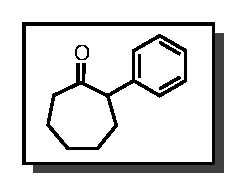
\includegraphics[scale=0.8]{chp_asymmetric/images/xaaa}
  \end{center}
  \vspace{-30pt}
\end{wrapfigure}
\textit{Representative procedure for racemic homologations:} \\ 
\textbf{\CMPxaaa}\ (\ref{cmp:xaaa}). In an inert atmosphere glovebox scandium triflate (6.2 mg,
0.012 mmol, 0.48 mol \%) was suspended in 0.4 mL of toluene. The suspension was moved to a nitrogen
manifold, and cyclohexanone (311 $\mu$L, 3.00 mmol, 1.19 equiv) was added in a single portion. The solution was stirred for 5 minutes at room temperature then cooled
to $-$78 \degc. Phenyldiazomethane \ref{cmp:diazoaa} (2.10 mL, 2.52 mmol, 1.20 M
in toluene, 1.00 equiv) was added, and the reaction mixture was warmed to 0 \degc. An 18
gauge exit needle was used to relieve excess pressure generated by the copious amounts of
nitrogen gas evolved. After 15 minutes, the pale yellow solution was diluted
with 30 mL of ether, washed with \ce{H2O} (20 mL), brine (20 mL), dried over
\ce{Na2SO4}, filtered, and concentrated. Purification by column chromatography
(8\% ethyl acetate in hexanes v/v) afforded the desired compound \ref{cmp:xaaa} as a
colorless oil (436 mg, 91.9\%) that solidified just below room temperature.\\
R$_f$ = 0.20 (10\% ethyl acetate in hexanes); 
$^1$H NMR (\ce{CDCl3}, 400 MHz) $\delta$ 7.35-7.29 (m, 2H), 7.27-7.21 (m, 3H),
3.73 (dd, \textit{J} =  11.3, 4.1 Hz, 1H), 2.70 (ddd, \textit{J} =  13.3, 13.3, 3.1 Hz, 1H), 2.57-2.49 (m, 1H), 2.20-2.11 (m, 1H), 2.10-1.91 (m, 4H), 1.72-1.58 (m, 1H), 1.54-1.40 (m, 2H); 
$^{13}$C NMR (CDCl$_3$, 100 MHz) $\delta$ 213.6, 140.5, 128.6, 128.0, 127.0,
58.9, 42.8, 32.1, 30.1, 28.7, 25.4; IR (neat) 3028 (w), 2929 (m), 2855 (w), 1702 (s),
1495 (w), 1452 (m), 719 (w), 698 (m) cm$^{-1}$; HRMS (ESI+) Calcd. for
\ce{C13H17O} [M+H]$^+$: 189.1279; Found 189.1277.

\vspace{10pt}
%***************[xaab]%***************%
\begin{wrapfigure}{l}{1.1in}
  \vspace{-25pt}
  \begin{center}
    
\includegraphics[scale=0.8]{chp_asymmetric/images/xaab}
  \end{center}
  \vspace{-30pt}
\end{wrapfigure}\noindent \textbf{\CMPxaab}\ (\ref{cmp:xaab}). Prepared according to the
representative procedure above using \ce{Sc(OTf)3} (24.6 mg, 0.0500 mmol, 1.00 mol \%)
suspended in 16.1 mL of \ce{CH2Cl2}, cyclobutanone (411 $\mu$L, 5.50 mmol, 1.10
equiv), and \ref{cmp:diazoab} (11.4 mL, 5.0 mmol, 0.44 M in toluene,
1.00 equiv).
Purification by column chromatography afforded \ref{cmp:xaab} as a colorless oil
(857 mg, 98.3\%). \\
R$_f$ = 0.33 (10\% ethyl acetate in hexanes); $^1$H NMR (500 MHz, \ce{CDCl3})
$\delta$ 7.37-7.30 (m, 4H), 7.25-7.21 (m, 1H), 2.58-2.53 (m, 1H), 2.37-2.33 (m, 2H), 2.05-1.84
 (m, 3H), 1.39 (s, 3H); $^{13}$C NMR (\ce{CDCl3}, 125 MHz) $\delta$ 220.77,
 142.75, 128.69, 126.78, 126.41, 53.23, 38.22, 37.76, 25.16, 18.86; IR (neat)
 2965 (bm), 2870 (bw), 1735 (s), 1496 (m), 1445 (m), 1156 (m), 1056 (m), 760 (m), 670 (m), 545
 (bm) cm$^{-1}$; HRMS (ESI+) Calcd. for \ce{C12H15O} [M+H]$^+$: 175.1123; Found
 175.1128.
%***************[xaab]%***************%

\vspace{10pt}
%***************[xaac]%***************%
\begin{wrapfigure}{l}{1.1in}
  \vspace{-25pt}
  \begin{center}
    
\includegraphics[scale=0.8]{chp_asymmetric/images/xaac}
  \end{center}
  \vspace{-30pt}
\end{wrapfigure}\noindent \textbf{\CMPxaac}\ (\ref{cmp:xaac}). Prepared
according to the representative procedure above using \ce{Sc(OTf)3} (24.6 mg,
0.0500 mmol, 1.00 mol
\%) suspended in 6.2 mL of \ce{CH2Cl2}, cyclobutanone (392 $\mu$L, 5.25 mmol,
1.05 equiv), and \ref{cmp:diazoaa} (3.76 mL, 5.00 mmol, 1.33 M in toluene, 1.00
equiv). Purification by column chromatography afforded \ref{cmp:xaac} as a
white solid (794 mg, 99.2\%), mp 37-39 \degc. \\
R$_f$ = 0.33 (20\% ethyl acetate in hexanes); $^1$H NMR (500 MHz, \ce{CDCl3})
$\delta$ 7.36-7.31 (m, 2H), 7.27-7.23 (m, 1H), 7.21-7.18 (m, 2H), 3.33 (dd, \textit{J} =
11.7, 8.8 Hz, 1H), 2.55-2.44 (m, 2H), 2.30 (ddd, \textit{J} = 19.5, 10.7, 8.8
Hz, 1H), 2.21-2.08 (m, 2H), 1.99-1.89 (m, 1H); $^{13}$C NMR (\ce{CDCl3}, 125
MHz) $\delta$ 218.20, 138.57, 128.73, 128.27, 127.03, 55.45, 38.58, 31.89,
21.00; IR (neat) 2961 (bw), 1737 (s), 1495 (m), 1452 (m), 1269 (bw), 1141 (m),
756 (m), 698 (s), 535 (m) cm$^{-1}$; HRMS (ESI+) Calcd.	for	\ce{C11H13O}
[M+H]$^+$: 161.0966; Found 161.0960.
%***************[xaac]%***************%

\vspace{10pt}
%***************[xaad]%***************%
\begin{wrapfigure}{l}{1.1in}
  \vspace{-25pt}
  \begin{center}
    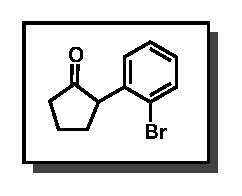
\includegraphics[scale=0.8]{chp_asymmetric/images/xaad}
  \end{center}
  \vspace{-30pt}
\end{wrapfigure}\noindent \textbf{\CMPxaad}\ (\ref{cmp:xaad}). Prepared
according to the representative procedure above using \ce{Sc(OTf)3} (4.9 mg,
0.010 mmol, 1.0 mol \%) suspended in 0.4 mL of \ce{CH2Cl2}, cyclobutanone (82
$\mu$L, 1.1 mmol, 1.1 equiv), and \ref{cmp:diazoac} (1.6 mL, 1.0 mmol, 0.64 M in
toluene, 1.0 equiv). Purification by column chromatography afforded
\ref{cmp:xaad} as a white solid (228 mg, 95.4\%), mp 50-53 \degc. \\
R$_f$ = 0.35 (20\% ethyl acetate in hexanes); $^1$H NMR (500 MHz, \ce{CDCl3})
$\delta$ 7.57 (dd, \textit{J} =  8.0, 1.5 Hz, 1H), 7.27 (ddd, \textit{J} =  7.6, 7.6, 1.5 Hz, 1H),
7.11 (ddd, \textit{J} =  7.6, 7.6, 1.7 Hz, 1H), 7.07 (dd, \textit{J} =  7.6, 1.7
Hz, 1H), 3.80-3.74 (m, 1H), 2.60-2.49 (m, 2H), 2.41-2.32 (m, 1H), 2.22-2.15 (m,
1H), 2.08-1.92 (m, 2H); $^{13}$C NMR (\ce{CDCl3}, 125 MHz) $\delta$ 217.54,
138.90, 133.20, 129.80, 128.67, 127.89, 125.23, 56.32, 38.74, 31.92, 21.03; IR
(neat) 2964 (bm), 2879 (bw), 1740 (s), 1474 (m), 1438 (m), 1163 (m), 1146
(m),1022 (m), 825 (w), 754 (m) cm$^{-1}$; HRMS (ESI+) Calcd. for \ce{C11H12BrO}
[M+H]$^+$: 239.0072; Found 239.0079. 

%***************[xaad]%***************%

\vspace{10pt}
%***************[xaae]%***************%
\begin{wrapfigure}{l}{1.15in}
  \vspace{-25pt}
  \begin{center}
    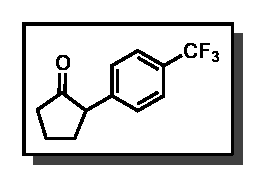
\includegraphics[scale=0.8]{chp_asymmetric/images/xaae}
  \end{center}
  \vspace{-30pt}
\end{wrapfigure}\noindent \textbf{\CMPxaae}\ (\ref{cmp:xaae}). Prepared
according to the representative procedure above using \ce{Sc(OTf)3} (4.9 mg,
0.010 mmol, 1.0 mol \%) suspended in 1.1 mL of \ce{CH2Cl2}, cyclobutanone (82
$\mu$L, 1.1 mmol, 1.1 equiv), and \ref{cmp:diazoad} (943 $\mu$L, 1.00 mmol, 1.06
M in toluene, 1.00 equiv). Purification by column chromatography afforded
\ref{cmp:xaae} as a white solid (209 mg, 91.6\%), mp 33-35 \degc. \\
R$_f$ = 0.30
(20\% ethyl acetate hexanes); $^1$H NMR (500
MHz, \ce{CDCl3}) $\delta$ 7.59 (d, \textit{J} = 8.3 Hz, 1H), 7.32 (d,
\textit{J} = 8.1 Hz, 1H), 3.39 (dd, \textit{J} = 12.0, 8.8 Hz, 1H), 2.58-2.47 (m, 2H),
2.31 (ddd, \textit{J} = 19.3, 10.5, 8.5 Hz, 1H), 2.24-2.08 (m, 2H), 2.02-1.92
(m, 1H); $^{13}$C NMR (\ce{CDCl3}, 125 MHz) $\delta$ 216.98, 142.41, 129.35 (q,
\textit{J}$_{C\mbox{-}F}$ = 32.2 Hz), 128.64, 125.63 (q,
\textit{J}$_{C\mbox{-}F}$ = 4.1 Hz), 124.31 (q, \textit{J}$_{C\mbox{-}F}$ =
272.0 Hz), 55.19, 38.44, 31.57, 20.94; IR (neat) 2967 (bw), 2883 (bw), 1743 (m),
1619 (w), 1326 (s), 1163 (m), 1120 (bs), 1069 (m), 840 (w) cm$^{-1}$; HRMS
(ESI+) Calcd. for \ce{C12H12F3O} [M+H]$^+$: 229.0840; Found 229.0848.
%***************[xaae]%***************%

\vspace{10pt}
% ***************[xaaf]%***************%
\begin{wrapfigure}{l}{1.25in}
  \vspace{-25pt}
  \begin{center}
    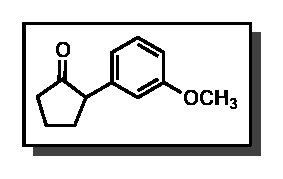
\includegraphics[scale=0.8]{chp_asymmetric/images/xaaf}
  \end{center}
  \vspace{-30pt}
\end{wrapfigure}\noindent \textbf{\CMPxaaf}\ (\ref{cmp:xaaf}). Prepared
according to the representative procedure above using \ce{Sc(OTf)3} (4.9 mg,
0.010 mmol, 1.0 mol \%) suspended in 1.1 mL of \ce{CH2Cl2}, cyclobutanone (82
$\mu$L, 1.1 mmol, 1.1 equiv), and \ref{cmp:diazoae} (943 $\mu$L, 1.00 mmol, 1.06
M in toluene, 1.00 equiv). Purification by column chromatography afforded
\ref{cmp:xaaf} as a colorless oil (167 mg, 87.8\%). \\
R$_f$ = 0.24 (20\% ethyl acetate in hexanes); $^1$H NMR (500 MHz, \ce{CDCl3})
$\delta$ 7.25 (dd, \textit{J} = 7.8, 7.8 Hz, 1H), 6.81-6.77 (m, 2H), 6.75 (dd,
\textit{J} = 2.2, 2.2 Hz, 1H), 3.80 (s, 3H), 3.30 (dd, \textit{J} = 11.7, 9.0
Hz, 1H), 2.54-2.43 (m, 2H), 2.30 (ddd, \textit{J} = 19.5, 11.0, 9.0 Hz, 1H),
2.20-2.07 (m, 2H), 1.98-1.87 (m, 1H); $^{13}$C NMR (\ce{CDCl3}, 125 MHz)
$\delta$ 217.95, 159.85, 140.10, 129.68, 120.58, 114.30, 112.26, 55.39, 55.32,
38.57, 31.85, 20.98; IR (neat) 2961 (bm), 2875 (bw), 1739 (s), 1601 (m), 1583
(m), 1490 (m), 1245 (bm), 1159 (m), 1041 (bm), 779 (bm), 695 (m) cm$^{-1}$; HRMS
(ESI+) Calcd. for \ce{C12H15O2} [M+H]$^+$: 191.1072; Found 191.1081.
%***************[xaaf]%***************%

\vspace{10pt}
%***************[xaag]%***************%
\begin{wrapfigure}{l}{1.1in}
  \vspace{-25pt}
  \begin{center}
    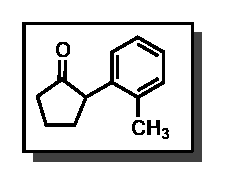
\includegraphics[scale=0.8]{chp_asymmetric/images/xaag}
  \end{center}
  \vspace{-30pt}
\end{wrapfigure}\noindent \textbf{\CMPxaag}\ (\ref{cmp:xaag}). Prepared
according to the representative procedure above using \ce{Sc(OTf)3} (4.9 mg,
0.010 mmol, 1.0 mol \%) suspended in 1.2 mL of \ce{CH2Cl2}, cyclobutanone (82
$\mu$L, 1.1 mmol, 1.1 equiv), and \ref{cmp:diazoaf} (769 $\mu$L, 1.00 mmol,
1.30 M in toluene, 1.00 equiv). Purification by column chromatography afforded
\ref{cmp:xaag} as a colorless oil (162 mg, 93.0\%).\\
R$_f$ = 0.36 (20\% ethyl acetate in hexanes); $^1$H NMR (500 MHz, \ce{CDCl3})
$\delta$ 7.20-7.13 (m, 3H), 7.01-6.99 (m, 1H), 3.53 (dd, \textit{J} = 11.7, 8.0
Hz, 1H), 2.54-2.45 (m, 2H), 2.33 (ddd, \textit{J} = 19.5, 10.8, 8.9 Hz, 1H),
2.32 (s, 3H), 2.22-2.15 (m, 1H), 2.09-1.91 (m, 2H); $^{13}$C NMR (\ce{CDCl3},
125 MHz) $\delta$ 218.81, 137.68, 136.90, 130.67, 127.46, 127.01, 126.40, 53.12,
38.82, 31.82, 21.17, 20.04; IR (neat) 2963 (bm), 2879 (bw), 1740 (s), 1493 (w),
1461 (bw), 1146 (m), 756 (m), 727 (m) cm$^{-1}$; HRMS (ESI+) Calcd. for
\ce{C12H15O} [M+H]$^+$: 175.1123; Found 175.1122. 
%***************[xaag]%***************%

\vspace{10pt}
%***************[xaah]%***************%
\begin{wrapfigure}{l}{1.1in}
  \vspace{-25pt}
  \begin{center}
    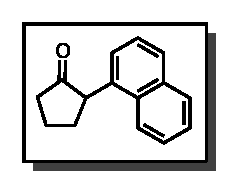
\includegraphics[scale=0.8]{chp_asymmetric/images/xaah}
  \end{center}
  \vspace{-30pt}
\end{wrapfigure}\noindent \textbf{\CMPxaah}\ (\ref{cmp:xaah}). Prepared
according to the representative procedure above using \ce{Sc(OTf)3} (4.9 mg,
0.010 mmol, 1.0 mol \%) suspended in 0.3 mL of \ce{CH2Cl2}, cyclobutanone (82
$\mu$L, 1.1 mmol, 1.1 equiv), and \ref{cmp:diazoag} (1.7 mL, 1.0 mmol, 0.58 M in
toluene, 1.0 equiv). Purification by column chromatography afforded
\ref{cmp:xaah} as a white solid (200 mg, 95.1\%), mp 93-95 \degc.\\
R$_f$ = 0.27 (20\% ethyl acetate in hexanes); $^1$H NMR (500 MHz, \ce{CDCl3})
$\delta$ 7.91-7.85 (m, 2H), 7.77 (d, \textit{J} =  8.3 Hz, 1H), 7.53-7.47 (m, 2H), 7.43
(dd, \textit{J} =  8.3, 7.3 Hz, 1H), 7.25 (dd, \textit{J} =  7.3, 1.0 Hz, 1H),
4.08 (dd, \textit{J} =  8.8, 8.8 Hz), 2.68-2.56 (m, 2H), 2.52-2.43 (m, 1H),
2.28-2.17 (m, 2H), 2.13-2.02 (m, 1H); $^{13}$C NMR (\ce{CDCl3}, 125 MHz)
$\delta$ 218.73, 135.58, 134.23, 132.20, 129.10, 127.78, 126.20, 125.78, 125.62,
125.18, 123.75, 52.44, 39.13, 32.56, 21.30; IR (neat) 2964 (bw), 1738 (s), 1510
(w), 1400 (m), 1142 (m), 1114 (m), 798 (m), 778 (s) cm$^{-1}$; HRMS (ESI+)
Calcd. for \ce{C15H15O} [M+H]$^+$: 211.1123; Found 211.1129.
%***************[xaah]%***************%

\vspace{10pt}
%***************[xaai]%***************%
\begin{wrapfigure}{l}{1.1in}
  \vspace{-15pt}
  \begin{center}
    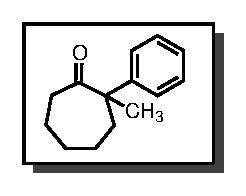
\includegraphics[scale=0.8]{chp_asymmetric/images/xaai}
  \end{center}
  \vspace{-30pt}
\end{wrapfigure}\noindent \textbf{\CMPxaai}\ (\ref{cmp:xaai}). Prepared
according to the representative procedure above using \ce{Sc(OTf)3} (4.9 mg,
0.010 mmol, 1.0 mol \%), cyclohexanone (114 $\mu$L, 1.10 mmol, 1.10 equiv), and
\ref{cmp:diazoab} (2.3 mL, 1.0 mmol, 0.44 M in toluene, 1.0 equiv). Purification
by column chromatography afforded \ref{cmp:xaai} as a colorless oil (206 mg,
quantitative). \\
R$_f$ = 0.43 (10\% ethyl acetate in hexanes); $^1$H NMR (500 MHz, \ce{CDCl3})
$\delta$ 7.34- 7.30 (m, 2H), 7.25-7.20 (m, 3H), 2.55 (ddd, \textit{J} = 13.7,
11.2, 2.7 Hz, 1H), 2.34-2.28 (m, 1H), 2.22-2.17 (m, 2H), 1.99-1.91 (m, 1H),
1.88-1.80 (m, 2H), 1.57-1.39 (m, 2H), 1.35 (s, 3H), 1.33-1.24 (m, 1H); $^{13}$C
NMR (\ce{CDCl3}, 125 MHz) $\delta$ 215.16, 145.09, 128.83, 126.74, 126.09,
55.97, 41.05, 36.77, 30.78, 27.10, 26.68, 24.49; IR (neat) 2930 (bm), 2858 (bw),
1702 (s), 1495 (w), 1458 (m), 764 (m), 700 (m) cm$^{-1}$; HRMS (ESI+) Calcd. for
\ce{C14H19O} [M+H]$^+$: 203.1436; Found 203.1443.
%***************[xaai]%***************%

\vspace{10pt}
%***************[xaaj]%***************%
\begin{wrapfigure}{l}{1.1in}
  \vspace{-30pt}
  \begin{center}
    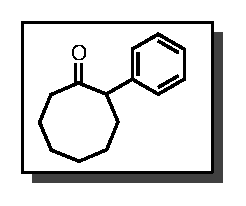
\includegraphics[scale=0.8]{chp_asymmetric/images/xaaj}
  \end{center}
  \vspace{-35pt}
\end{wrapfigure}\noindent \textbf{\CMPxaaj}\ (\ref{cmp:xaaj}). Prepared
according to the representative procedure above using \ce{Sc(OTf)3} (24.6 mg,
0.0500 mmol, 1.00 mol \%) suspended in 5.8 mL of toluene, cycloheptanone (710
$\mu$L, 6.00 mmol, 1.20 equiv), and \ref{cmp:diazoaa} (4.17 mL, 5.00 mmol, 1.20
M in toluene, 1.00 equiv). Purification by column chromatography afforded
\ref{cmp:xaaj} as a white solid (903 mg, 89.2\%), mp 36-38 \degc. \\
R$_f$ = 0.33 (10\% ethyl acetate in hexanes); $^1$H NMR (\ce{CDCl3}, 400 MHz)
$\delta$ 7.36-7.28 (m, 4H), 7.26-7.20 (m, 1H), 3.79 (dd, \textit{J} = 12.3, 2.7
Hz, 1H), 2.61 (ddd, \textit{J} = 12.5, 12.5, 4.3 Hz, 1H), 2.42- 2.30 (m, 1H),
2.29-2.22 (m, 1H), 2.04-1.86 (m, 3H), 1.83-1.70 (m, 2H), 1.65-1.55 (m, 2H),
1.53-1.37 (m, 2H); $^{13}$C NMR (\ce{CDCl3}, 100 MHz) $\delta$ 216.57, 139.49,
128.64, 127.91, 127.12, 57.53, 40.40, 31.67, 26.98, 26.88, 26.85, 24.76; IR (neat) 2927
(s), 2855 (w), 1698 (s), 1494 (w), 1449 (m), 700 (m) cm$^{-1}$; HRMS (ESI+)
Calcd. for \ce{C14H19O} [M+H]$^+$: 203.1436; Found: 203.1439.
%***************[xaaj]%***************%

\vspace{10pt}
%***************[xaak]%***************%
\begin{wrapfigure}{l}{1.1in}
  \vspace{-23pt}
  \begin{center}
    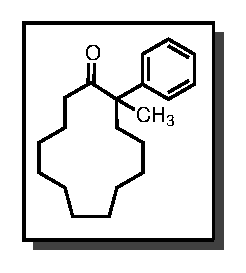
\includegraphics[scale=0.8]{chp_asymmetric/images/xaak}
  \end{center}
  \vspace{-30pt}
\end{wrapfigure}\noindent \textbf{\CMPxaak}\ (\ref{cmp:xaak}). Prepared
according to to the representative procedure above using \ce{Sc(OTf)3} (24.6 mg,
0.0500 mmol, 7.00 mol \%), however, rather then suspending the \ce{Sc(OTf)3} in
solvent, cyclododecanone (145 mg, 0.715 mmol, 1.00 equiv) was introduced to the
\ce{Sc(OTf)3} as a solution in 1.8 mL of \ce{CH2Cl2}. The rest of the procedure
was carried out as usual with \ref{cmp:diazoab} (1.8 mL, 0.79 mmol, 0.44 M in
toluene, 1.1 equiv). Purification by column chromatography afforded
\ref{cmp:xaak} as a colorless semi-solid (191 mg, 83.8\%). \\
R$_f$ = 0.43 (10\% ethyl acetate in hexanes); $^1$H NMR (500 MHz, \ce{CDCl3})
$\delta$ 7.34-7.29 (m, 2H), 7.27-7.20 (m, 3H), 2.37 (ddd, \textit{J} =  18.3, 9.0, 4.2 Hz,
1H), 2.24 (ddd, \textit{J} =  12.9, 12.9, 3.2 Hz, 1H), 1.98 (dddd, \textit{J} = 
18.3, 4.6, 4.6, 4.6 Hz, 1H), 1.90 (ddd, \textit{J} =  13.2, 13.2, 5.6 Hz, 1H),
1.84-1.76 (m, 1H), 1.61-1.54 (m, 1H), 1.51-1.39 (m, 2H), 1.38-1.22 (m, 11H),
1.36 (s, 3H), 1.21-1.14 (m, 1H), 1.14-1.03 (m, 2H); $^{13}$C NMR (\ce{CDCl3},
125 MHz) $\delta$ 213.65, 145.55, 128.73, 126.79, 126.50, 56.04, 36.86, 36.13,
27.56, 26.92, 26.64, 25.84, 25.72, 25.22, 24.75, 24.24, 22.26, 22.13; IR (neat)
2930 (bs), 2860 (bm), 1706 (s), 1495 (m), 1463 (m), 1445 (m), 763 (m), 700 (m)
cm$^{-1}$; HRMS (ESI+)	Calcd.	for	\ce{C20H31O} [M+H]$^+$:	287.2375;	Found
287.2376.
%***************[xaak]%***************%

\vspace{10pt}
% ***************[xaax]%***************%
%%%%% numbered  as racemic xaay 
\begin{wrapfigure}{l}{1.40in}
  \vspace{-32pt}
  \begin{center}
    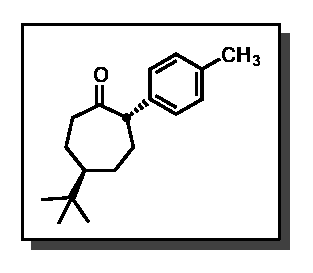
\includegraphics[scale=0.8]{chp_asymmetric/images/xaax}
  \end{center}
  \vspace{-35pt}
\end{wrapfigure}\noindent \textbf{\CMPxaax}\ (\ref{cmp:xaay}). Scandium triflate
(49.2 mg, 0.10 mmol, 10 mol \%) was suspended in 8 mL of toluene. To the stirred
suspension, 4-\textit{tert}-butylcyclohexanone (185 mg, 1.20 mmol, 1.20 equiv)
was transferred \textit{via} cannula in 2 mL of toluene without rinsing. After
stirring for 10 minutes at room temperature, the clear solution was cooled to
$-$78 \degc\ and \textit{p}-tolylphenyldiazomethane (1.5 mL, 1.0 mmol, 0.66 M in
toluene, 1.0 equiv) was added \textit{via} syringe. After 1 hour the pale yellow
reaction mixture was diluted with 25 mL of Et$_2$O then washed with 25 mL of
water and 25 mL of brine. The organics were dried over anhydrous Na$_2$SO$_4$
and concentrated to a faint yellow crude solid. Purification by flash column
chromatography (10\% ethyl acetate in hexanes) afforded the \textit{trans}
diastereomer ($\pm$)-\ref{cmp:xaay} as a white solid (227 mg, 87.8\%), mp 90-92 \degc.
Suitable crystals for X-ray analysis were grown by slow evaporation of a supersaturated hexanes solution. GC analysis of the crude reaction mixture showed a 96.5:3.5 dr (HP-5, 150 \degc\ hold 5 min, ramp 5 \degc/min to 200 \degc; t$_R$ = 16.9 min (minor), 17.4 min (major)). \\
R$_f$ = 0.30 (10\% ethyl acetate in hexanes); $^1$H NMR (CDCl$_3$, 400 MHz)
$\delta$ 7.16-7.09 (m, 4H), 3.67 (dd, \textit{J} = 11.9, 3.5 Hz, 1H), 2.68 (ddd,
\textit{J} =  16.2, 13.1, 3.3 Hz, 1H), 2.49 (ddd, \textit{J} = 9.2, 6.3, 2.7 Hz,
1H), 2.32 (s, 3H), 2.23-2.13 (m, 2H), 2.12-2.04 (m, 1H), 2.01-1.90 (m, 1H), 1.49-1.38 (m, 1H), 1.26-1.12 (m, 2H), 0.91 (s, 9H); $^{13}$C NMR (CDCl$_3$, 100 MHz) $\delta$ 214.10, 137.14, 136.66, 129.36, 127.74, 58.60, 52.16, 41.73, 33.67, 32.00, 29.76, 27.80, 26.94, 21.15; IR (neat) 2953 (bm), 2864 (bw), 1695 (s), 1513 (w), 1366 (w), 1235 (w), 828 (w), 797 (w) cm$^{-1}$; HRMS (ESI+) Calcd. for C$_{18}$H$_{27}$O [M+H]$^+$: 259.2062; Found: 259.2062.
%***************[xaax]%***************%

\pagebreak
%***************[xaal]%***************%
\begin{wrapfigure}{l}{1.1in}
  \vspace{-22pt}
  \begin{center}
    
\includegraphics[scale=0.8]{chp_asymmetric/images/xaal}
  \end{center}
  \vspace{-30pt}
\end{wrapfigure}\noindent \textit{Representative procedure for asymmetric
homologations:} \\ \textbf{\CMPxaal}\ (\ref{cmp:xaal}). In an inert atmosphere
glove box scandium triflate (30.4 mg, 0.0618 mmol, 5.00 mol \%) was weighed into
a 25 mL scintillation vial. Ligand \ref{cmp:ligandab} (35.0 mg, 0.0679 mmol,
5.50 mol \%) was transferred to the vial containing scandium triflate with 6.2
mL of toluene. The suspension was sealed with a rubber septum and stirred for
1.5 hours then removed from the glove box and to a nitrogen manifold.
Cycloheptanone (146 $\mu$L, 1.24 mmol, 1.00 equiv) was added to the cloudy gray
suspension and stirred for 15 minutes at which point the reaction mixture became
clear and homogeneous. The reaction was cooled to $-$78~\degc\  and
phenyldiazomethane \ref{cmp:diazoaa} (1.20 mL, 1.48 mmol, 1.20 M in
toluene, 1.20 equiv) was added in a single portion. After 6 hours the cold
reaction mixture was quickly poured into 20 mL of water and diluted with 30 mL
of Et$_2$O. The organic layer was washed with 20 mL water, 20 mL of brine,
dried over anhydrous \ce{Na2SO4}, and concentrated to a crude yellow oil.
Purification by column chromatography (10\% ethyl acetate in hexanes) yielded \ref{cmp:xaal} as a white solid (235 mg, 94.0\%) with 97:3 er (AS-H,
50~\degc, 150 psi, 3.0 mL/min, 4\% MeOH, $\lambda$ = 220 nm; t$_R$ = 1.85 min
(minor), 2.07 min (major)). Characterization data were in agreement with those
tabulated above for the racemic compound. \rotation = $-$138.8 (c 1.26,
\ce{CHCl3}). \\
\begin{figure}[h]
\centering
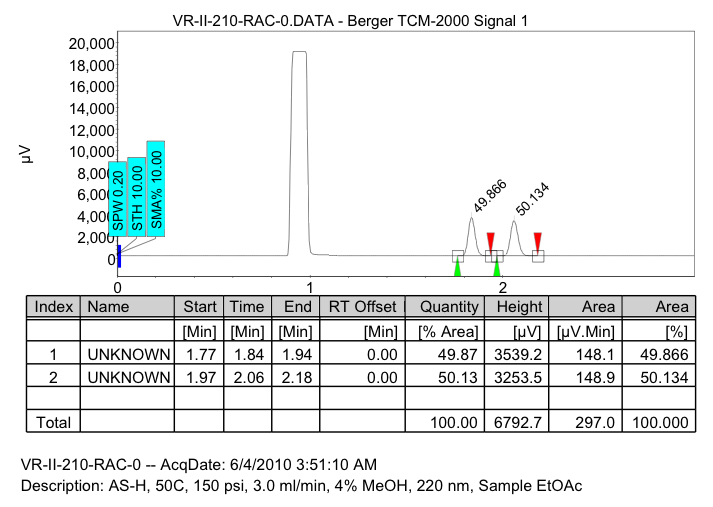
\includegraphics[width=2.75in]{chp_asymmetric/images/sfc/xaal-rac.png}
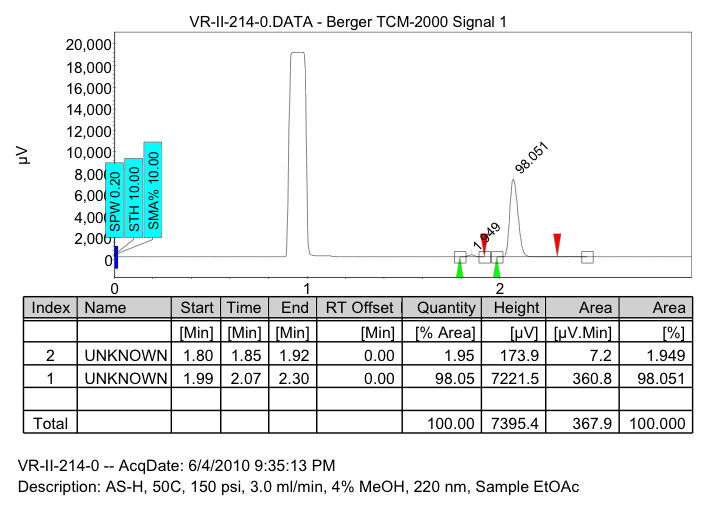
\includegraphics[width=2.75in]{chp_asymmetric/images/sfc/xaal.png}
\caption{SFC trace for \CMPxaal~(\ref{cmp:xaal})}
\vspace{-10pt}
\end{figure}
%***************[xaal]%***************%

\pagebreak
%***************[xaam]%***************%
\begin{wrapfigure}{l}{1.0in}
  \vspace{-15pt}
  \begin{center}
    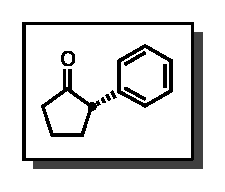
\includegraphics[scale=0.8]{chp_asymmetric/images/xaam}
  \end{center}
  \vspace{-25pt}
\end{wrapfigure}\noindent \textbf{\CMPxaam}\ (\ref{cmp:xaam}). Run for 1.5 hours
at $-$78 \degc\  according to the representative procedure with scandium
triflate (7.4 mg, 0.015 mmol, 10 mol \%), ligand \ref{cmp:ligandab} (8.5 mg, 0.016 mmol,
11 mol \%), toluene (1.5 mL), cyclobutanone (16 $\mu$L, 0.18 mmol, 1.2 equiv),
and \ref{cmp:diazoaa} (203 $\mu$L, 0.15 mmol, 0.74 M in toluene, 1.0 equiv). The
crude reaction mixture was not purified by column
chromatography,\footnote{Tertiary $\alpha$-aryl
cyclopentanones are known to racemize on silica gel. See
reference \ref{ref:asshitertiary} for details.} but instead poured into 15 mL of
pentane and filtered through a cotton plug. The organics were washed with 10 mL of water, 10 mL of brine, and dried over \ce{Na2SO4}.
Concentration under high vacuum afforded a crude yellow oil that was taken up in
1.5 mL of hexanes and again filtered through a cotton plug. Concentration
afforded \ref{cmp:xaam} as a pale yellow oil (26.2 mg, quantitative) with
85.5:14.5 er (AS-H, 50 \degc, 150 psi, 1.5 mL/min, 2\% MeOH, $\lambda$ = 220 nm;
t$_R$ = 4.02 min (minor), 4.67 min (major)). Characterization data were in agreement with those tabulated above for the racemic compound. \\
\begin{figure}[h]
\centering
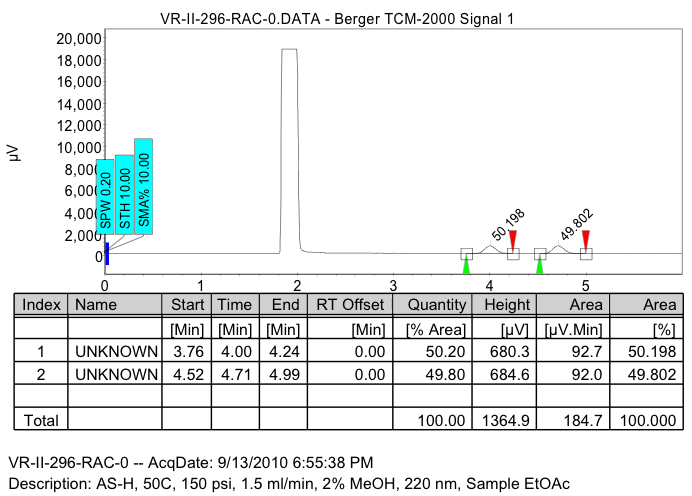
\includegraphics[width=2.75in]{chp_asymmetric/images/sfc/xaam-rac.png}
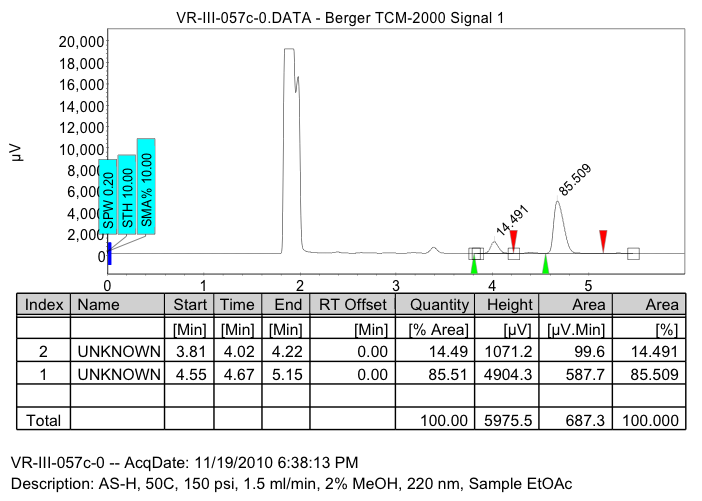
\includegraphics[width=2.75in]{chp_asymmetric/images/sfc/xaam.png}
\caption{SFC trace for \CMPxaam~(\ref{cmp:xaam})}
\vspace{-10pt}
\end{figure}
%***************[xaam]%***************%

\pagebreak
%***************[xaan]%***************%
\begin{wrapfigure}{l}{1.05in}
  \vspace{-22pt}
  \begin{center}
    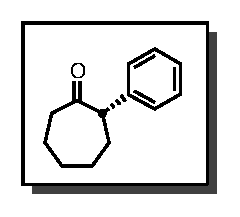
\includegraphics[scale=0.8]{chp_asymmetric/images/xaan}
  \end{center}
  \vspace{-30pt}
\end{wrapfigure}\noindent \textbf{\CMPxaan}\ (\ref{cmp:xaan}). Run for 1.5 hours
at $-$78 \degc\  according to the representative procedure with scandium triflate (7.4
mg, 0.015 mmol, 10 mol \%), ligand \ref{cmp:ligandab} (8.5 mg, 0.016 mmol, 11
mol \%), toluene (1.5 mL), cyclohexanone (19 $\mu$L, 0.18 mmol, 1.2 equiv), and
\ref{cmp:diazoaa} (203 $\mu$L, 0.15 mmol, 0.74 M in toluene, 1.0 equiv). The
crude reaction mixture was directly purified by column chromatography to afford
\ref{cmp:xaan} as a colorless oil (26.5 mg, 94.0\%) with 95:5 er (AS-H, 50
\degc, 150 psi, 3.0 mL/min, 2\% MeOH, $\lambda$ = 220 nm; t$_R$ = 2.35 min
(minor), 2.70 min (major)). Characterization data were in agreement with those
tabulated above for the racemic compound. \rotation = $-$138.2 (c 0.80,
CHCl$_3$).
\\
\begin{figure}[h]
\centering
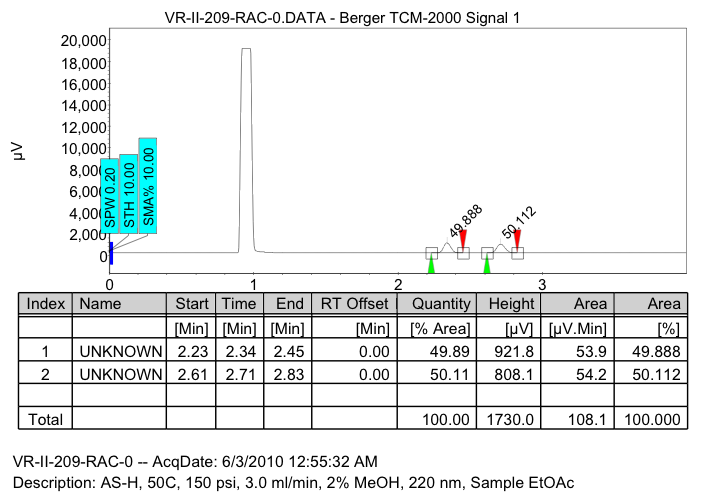
\includegraphics[width=2.75in]{chp_asymmetric/images/sfc/xaan-rac.png}
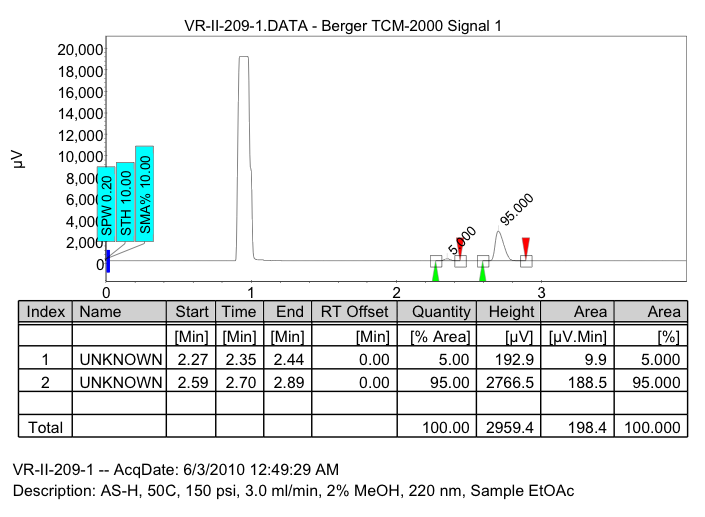
\includegraphics[width=2.75in]{chp_asymmetric/images/sfc/xaan.png}
\caption{SFC trace for \CMPxaan~(\ref{cmp:xaan})}
\vspace{-10pt}
\end{figure}
%***************[xaan]%***************%

\pagebreak
%***************[xaao]%***************%
\begin{wrapfigure}{l}{1.35in}
  \vspace{-22pt}
  \begin{center}
    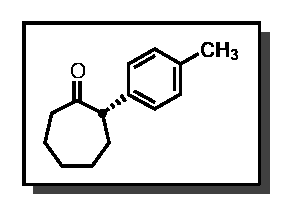
\includegraphics[scale=0.8]{chp_asymmetric/images/xaao}
  \end{center}
  \vspace{-30pt}
\end{wrapfigure}\noindent \textbf{\CMPxaao}\ (\ref{cmp:xaao}). Run for 1.5 hours
at $-$78 \degc\  according to the representative procedure with scandium triflate (7.4
mg, 0.015 mmol, 10 mol \%), ligand \ref{cmp:ligandab} (8.5 mg, 0.016 mmol, 11
mol \%), toluene (1.5 mL), cyclohexanone (19 $\mu$L, 0.18 mmol, 1.2 equiv), and
\ref{cmp:diazoah} (227 $\mu$L, 0.15 mmol, 0.66 M in toluene, 1.0 equiv). The
crude reaction mixture was directly purified by column chromatography to afford
\ref{cmp:xaao} as a colorless oil (29.2 mg, 96.4\%) with 94:6 er (AS-H, 50
\degc, 150 psi, 3.0 mL/min, 2\% MeOH, $\lambda$ = 220 nm; t$_R$ = 2.49 min
(minor), 2.90 min (major)).\\
\noindent  \rotation = $-$154.5 ($c$ 0.47, CHCl$_3$); R$_f$ = 0.18 (10\% ethyl
acetate in hexanes); $^1$H NMR (CDCl$_3$, 400 MHz) $\delta$ 7.16-7.10 (m, 4H), 3.69 (dd, \textit{J} = 11.3, 4.1 Hz, 1H), 2.73-2.64 (m, 1H), 2.55-2.47 (m, 1H), 2.32 (s,
3H), 2.18-2.08 (m, 1H), 2.08-1.89 (m, 4H), 1.70-1.56 (m, 1H), 1.52-1.40 (m, 2H); $^{13}$C NMR (CDCl$_3$, 100 MHz) $\delta$ 213.77, 137.46, 136.61, 129.35, 127.80, 58.56, 42.71, 32.04, 30.18, 28.63, 25.51; IR (neat) 3022 (bw), 2927 (bm), 2856 (w), 1702 (s), 1513 (m), 1454 (bm), 1163 (w), 1129 (w), 825 (w), 789 (w) cm$^{-1}$; HRMS (ESI+) Calcd. for C$_{14}$H$_{19}$O [M+H]$^+$: 203.1436; Found 203.1445.
\begin{figure}[h]
\centering
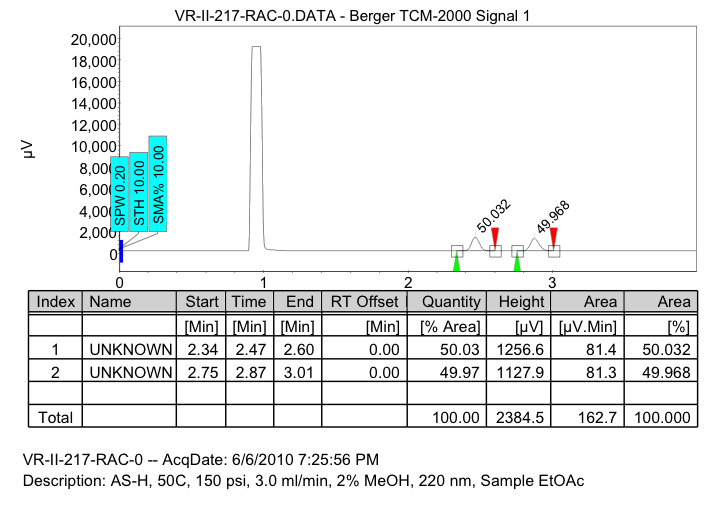
\includegraphics[width=2.75in]{chp_asymmetric/images/sfc/xaao-rac.png}
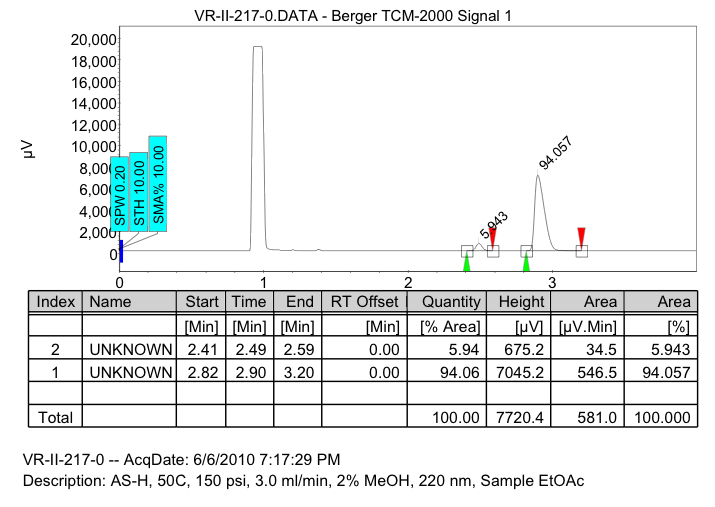
\includegraphics[width=2.75in]{chp_asymmetric/images/sfc/xaao.png}
\caption{SFC trace for \CMPxaao~(\ref{cmp:xaao})}
\vspace{-10pt}
\end{figure}
%***************[xaao]%***************%

\pagebreak
%***************[xaap]%***************%
\begin{wrapfigure}{l}{1.25in}
  \vspace{-22pt}
  \begin{center}
    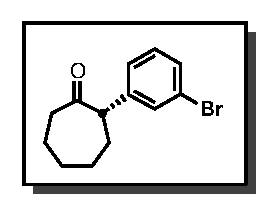
\includegraphics[scale=0.8]{chp_asymmetric/images/xaap}
  \end{center}
  \vspace{-30pt}
\end{wrapfigure}\noindent \textbf{\CMPxaap}\ (\ref{cmp:xaap}). Run for 3 hours
at $-$78 \degc\  according to the representative procedure with scandium triflate (7.4
mg, 0.015 mmol, 10 mol \%), ligand \ref{cmp:ligandab} (8.5 mg, 0.016 mmol, 11
mol \%), toluene (1.5 mL), cyclohexanone (19 $\mu$L, 0.18 mmol, 1.2 equiv), and
\ref{cmp:diazoai} (125 $\mu$L, 0.15 mmol, 1.20 M in toluene, 1.0 equiv). The
crude reaction mixture was directly purified by column chromatography to afford
\ref{cmp:xaap} as a colorless oil (41.1 mg, quantitative) with 94.5:5.5 er
(AS-H, 50 \degc, 150 psi, 3.0 mL/min, 3\% MeOH, $\lambda$ = 220 nm; t$_R$ = 3.02
min (minor), 3.58 min (major)).\\
\noindent  \rotation = $-$102.7 ($c$ 1.05, CHCl$_3$); R$_f$ = 0.27 (10\% ethyl
acetate in hexanes); $^1$H NMR (CDCl$_3$, 400 MHz) $\delta$ 7.38-7.34 (m, 2H),
7.20-7.12 (m, 2H), 3.70 (dd, \textit{J} = 11.2, 3.7 Hz, 1H), 2.69-2.60 (m, 1H),
2.59-2.51 (m, 1H), 2.14-1.86 (m, 5H), 1.72-1.59 (m, 1H), 1.54-1.38 (m, 2H);
$^{13}$C NMR (CDCl$_3$, 100 MHz) $\delta$ 212.67, 142.80, 131.11, 130.10,
130.07, 126.83, 122.63, 58.57, 43.06, 32.19, 29.87, 28.82, 25.10; IR (neat) 2928
(m), 2855 (w), 1702 (s), 1593 (w), 1566 (w), 1475 (w), 1454 (w), 1129 (w), 1074
(w), 937 (w), 779 (w), 690 (w) cm$^{-1}$; HRMS (ESI+) Calcd. for
C$_{13}$H$_{16}$BrO [M+H]$^+$: 269.0364; Found: 269.0401. \\
\begin{figure}[h]
\centering
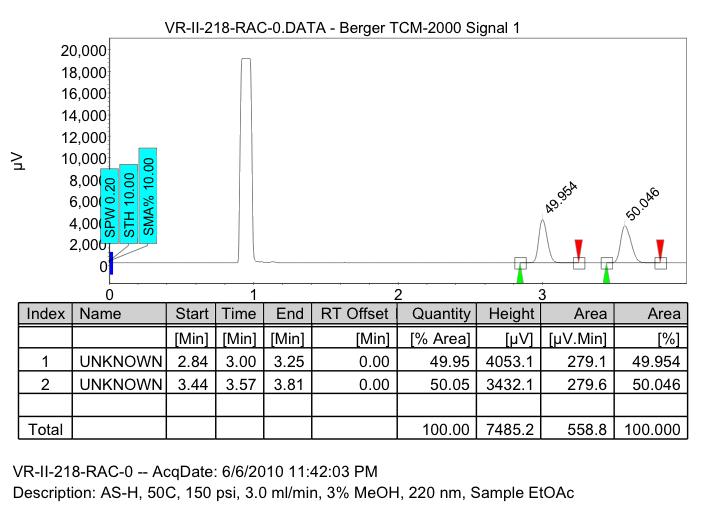
\includegraphics[width=2.75in]{chp_asymmetric/images/sfc/xaap-rac.png}
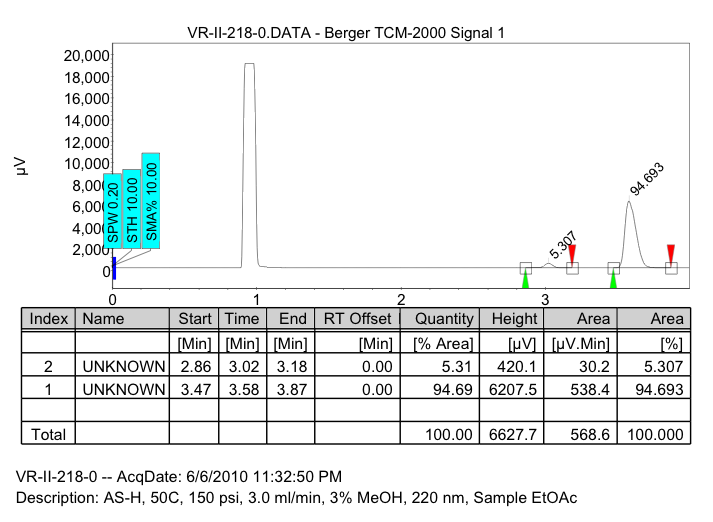
\includegraphics[width=2.75in]{chp_asymmetric/images/sfc/xaap.png}
\caption{SFC trace for \CMPxaap~(\ref{cmp:xaap})}
\vspace{-10pt}
\end{figure}
%***************[xaap]%***************%

\pagebreak
%***************[xaaq]%***************%
\begin{wrapfigure}{l}{1.2in}
  \vspace{-23pt}
  \begin{center}
    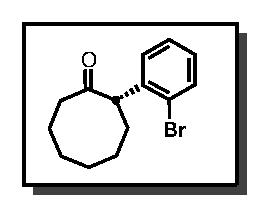
\includegraphics[scale=0.8]{chp_asymmetric/images/xaaq}
  \end{center}
  \vspace{-30pt}
\end{wrapfigure}\noindent \textbf{\CMPxaaq}\ (\ref{cmp:xaaq}). Run for 14 hours
at $-$78 \degc\  according to the representative procedure with scandium triflate (7.4
mg, 0.015 mmol, 10 mol \%), ligand \ref{cmp:ligandaa} (5.9 mg, 0.016 mmol, 11
mol \%), toluene (1.5 mL), cycloheptanone (18 $\mu$L, 0.15 mmol, 1.0 equiv), and
\ref{cmp:diazoac} (370 $\mu$L, 0.21 mmol, 0.57 M in toluene, 1.4 equiv). The
crude reaction mixture was directly purified by column chromatography to afford
\ref{cmp:xaaq} as a colorless oil (35.9 mg, 85.0\%) with 92.5:7.5 er
(AS-H, 50 \degc, 150 psi, 2.0 mL/min, 2\% MeOH, $\lambda$ = 220 nm; t$_R$ = 4.65
min (major), 5.09 min (minor)). \\ 
\rotation = $-$1.9 (c 0.99, CHCl$_3$); R$_f$ = 0.21 (10\% ethyl acetate in
hexanes); $^1$H NMR (CDCl$_3$, 400 MHz) $\delta$ 7.54-7.48 (m, 2H), 7.34-7.28
(m, 1H), 7.12-7.05 (m, 1H), 4.67 (dd, \textit{J} = 11.5, 3.3 Hz, 1H), 2.74 (ddd,
\textit{J} = 14.9, 7.4, 3.1 Hz, 1H), 2.49-2.40 (m, 1H), 2.39-2.25 (m, 1H),
2.15-2.04 (m, 1H), 2.03-1.88 (m, 2H), 1.86-1.66 (m, 3H), 1.65-1.52 (m, 2H),
1.37-1.24 (m, 1H); $^{13}$C NMR (CDCl$_3$, 100 MHz) $\delta$ 215.99, 139.78,
132.55, 130.04, 128.33, 127.68, 124.54, 52.89, 44.67, 35.56, 28.61, 25.74,
25.08, 23.87; IR (neat) 3063 (bw), 2927 (bm), 2856 (bw), 1705 (s), 1467 (m),
1440 (m), 1326 (w), 1157 (w), 1021 (m), 743 (m) cm$^{-1}$; HRMS (ESI+) Calcd.
for \ce{C14H18BrO} [M+H]$^+$: 281.0541; Found: 281.0571. \\
\begin{figure}[h]
\centering
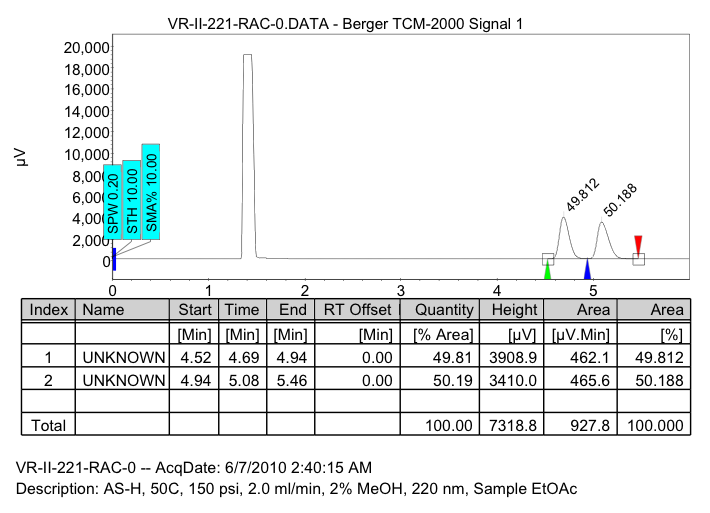
\includegraphics[width=2.75in]{chp_asymmetric/images/sfc/xaaq-rac.png}
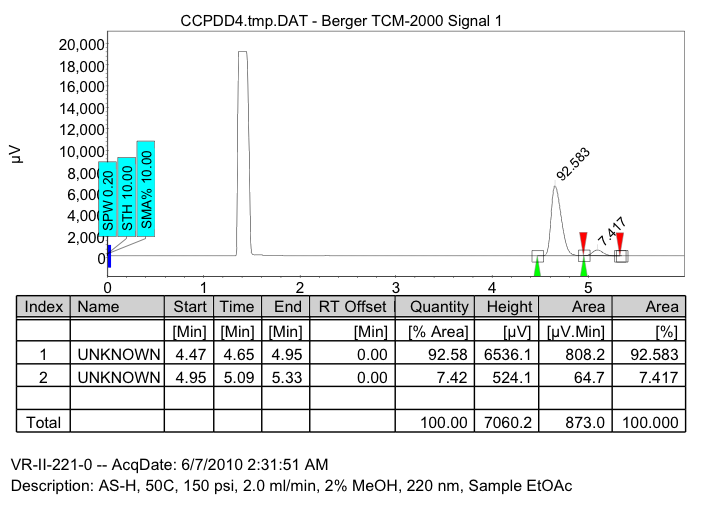
\includegraphics[width=2.75in]{chp_asymmetric/images/sfc/xaaq.png}
\caption{SFC trace for \CMPxaaq~(\ref{cmp:xaaq})}
\vspace{-10pt}
\end{figure}
%***************[xaaq]%***************%

\pagebreak
%***************[xaar]%***************%
\begin{wrapfigure}{l}{1.4in}
  \vspace{-12pt}
  \begin{center}
    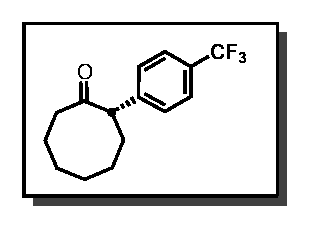
\includegraphics[scale=0.8]{chp_asymmetric/images/xaar}
  \end{center}
  \vspace{-25pt}
\end{wrapfigure}\noindent \textbf{\CMPxaar}\ (\ref{cmp:xaar}). Run for 14 hours
at $-$78 \degc\  according to the representative procedure with scandium
triflate (7.4 mg, 0.015 mmol, 10 mol \%), ligand \ref{cmp:ligandab} (8.5 mg,
0.016 mmol, 11 mol \%), toluene (1.5 mL), cycloheptanone (18 $\mu$L, 0.15 mmol,
1.0 equiv), and \ref{cmp:diazoad} (320 $\mu$L, 0.21 mmol, 0.66 M in toluene, 1.4
equiv).
The crude reaction mixture was directly purified by column chromatography to
afford \ref{cmp:xaar} as a colorless oil (31.7 mg, 78.3\%) with 98:2 er (AD-H,
50 \degc, 150 psi, 1.0 mL/min, 3\% MeOH, $\lambda$ = 220 nm; t$_R$ = 8.69 min
(minor), 9.44 min (major)). \\
\rotation = $-$93.52 (c 0.88, CHCl$_3$); R$_f$ = 0.18 (10\% ethyl acetate in
hexanes); $^1$H NMR (CDCl$_3$, 400 MHz) $\delta$ 7.56 (d, \textit{J} = 8.0 Hz, 1H), 7.46
(d, \textit{J} = 8.0 Hz, 1H), 3.92 (dd, \textit{J} = 12.1, 2.9 Hz, 1H), 2.55
(ddd, \textit{J} = 12.5, 12.5, 3.7 Hz, 1H), 2.38- 2.22 (m, 2H), 2.10-1.97 (m,
2H), 1.96-1.86 (m, 1H), 1.84-1.69 (m, 2H), 1.64-1.46 (m, 4H); $^{13}$C NMR
(CDCl$_3$, 100 MHz) $\delta$ 215.72, 143.67 (q, \textit{J}$_{C\mbox{-}F}$ = 1.5 Hz), 129.40 (q, \textit{J}$_{C\mbox{-}F}$
= 32.2 Hz), 128.44, 125.50 (q, \textit{J}$_{C\mbox{-}F}$ = 3.7 Hz), 124.30 (q, \textit{J}$_{C\mbox{-}F}$ = 271.5 Hz),
56.73, 41.40, 32.97, 27.22, 26.44, 26.18, 24.75; IR (neat) 2935 (bw), 2860 (bw),
1703 (m), 1617 (w), 1466 (w), 1447 (w), 1419 (w), 1325 (s), 1163 (m), 1122 (m),
1069 (m), 1019 (m), 838 (bw) cm$^{-1}$; HRMS (ESI+) Calcd. for \ce{C15H18F3O}
[M+H]$^+$: 271.1310; Found: 271.1341.  \\
\begin{figure}[h]
\centering
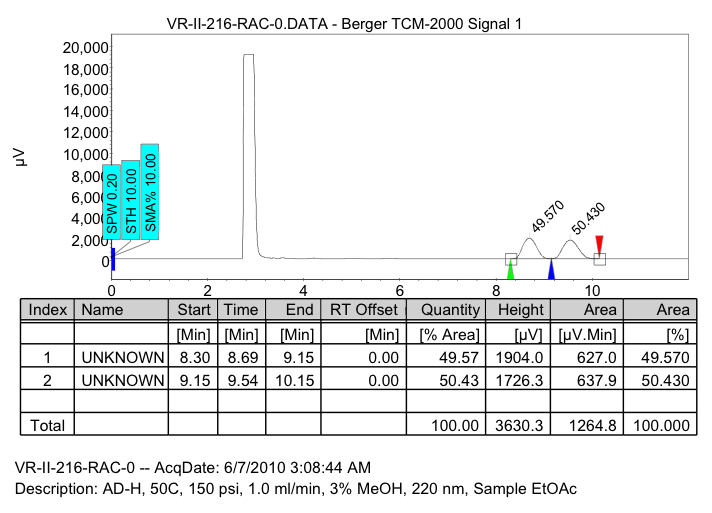
\includegraphics[width=2.75in]{chp_asymmetric/images/sfc/xaar-rac.png}
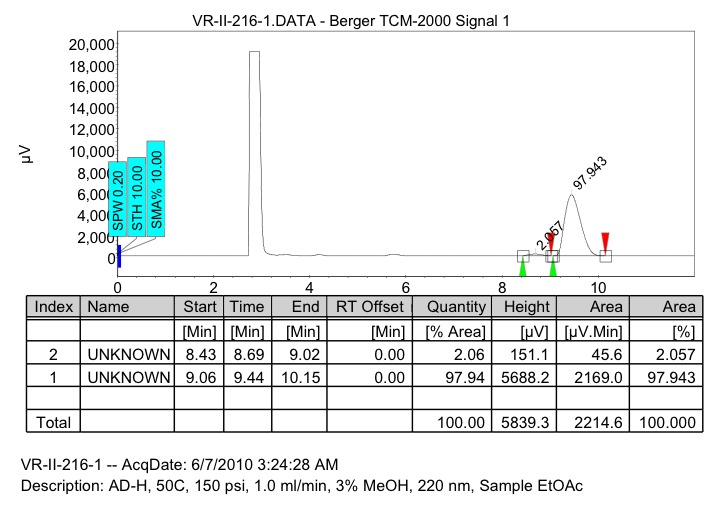
\includegraphics[width=2.75in]{chp_asymmetric/images/sfc/xaar.png}
\caption{SFC trace for \CMPxaar~(\ref{cmp:xaar})}
\vspace{-10pt}
\end{figure}
%***************[xaar]%***************%

\pagebreak
%***************[xaas]%***************%
\begin{wrapfigure}{l}{1.4in}
  \vspace{-12pt}
  \begin{center}
    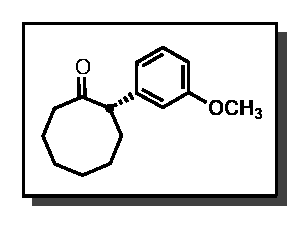
\includegraphics[scale=0.8]{chp_asymmetric/images/xaas}
  \end{center}
  \vspace{-25pt}
\end{wrapfigure}\noindent \textbf{\CMPxaas}\ (\ref{cmp:xaas}). Run for 3 hours
at $-$78 \degc\  according to the representative procedure with scandium
triflate (7.4 mg, 0.015 mmol, 10 mol \%), ligand \ref{cmp:ligandab} (8.5 mg, 0.016 mmol,
11 mol \%), toluene (1.5 mL), cycloheptanone (18 $\mu$L, 0.15 mmol, 1.0 equiv),
and \ref{cmp:diazoae} (200 $\mu$L, 0.21 mmol, 1.0 M in toluene, 1.4 equiv). The
crude reaction mixture was directly purified by column chromatography to afford
\ref{cmp:xaas} as a colorless oil (35.1 mg, quantitative) with 97:3 er (AS-H, 50
\degc, 150 psi, 2.0 mL/min, 2\% MeOH, $\lambda$ = 220 nm; t$_R$ = 2.05 min
(minor), 2.26 min (major)). \\
\rotation = $-$116.3 (c 0.99, CHCl$_3$); R$_f$ = 0.16 (10\% ethyl acetate in
hexanes); $^1$H NMR (CDCl$_3$, 400 MHz) $\delta$ 7.24-7.18 (m, 1H), 6.94-6.88
(m, 2H), 6.80-6.75 (m, 1H), 3.80 (s, 3H), 3.75 (dd, \textit{J} =  12.5, 2.7 Hz,
1H), 2.62 (ddd, \textit{J} =  11.7, 4.7 Hz, 1H), 2.41-2.29 (m, 1H), 2.29-2.21
(m, 1H), 2.03- 1.84 (m, 3H), 1.82-1.69 (m, 2H), 1.64-1.53 (m, 2H), 1.53-1.34 (m,
2H); $^{13}$C NMR (CDCl$_3$, 100 MHz) $\delta$ 216.41, 159.79, 140.98, 129.53,
120.21, 113.81, 112.41, 57.60, 55.31, 40.25, 31.44, 27.10, 26.87, 26.80, 24.74;
IR (neat) 2929 (s), 2856 (w), 1697 (s), 1598 (m), 1583 (m), 1491 (m), 1465 (m),
1286 (s), 1048 (m), 767 (w), 696 (w) cm$^{-1}$; HRMS (ESI+) Calcd. for
\ce{C15H21O2} [M+H]$^+$: 233.1542; Found: 233.1560. \\
\begin{figure}[h]
\centering
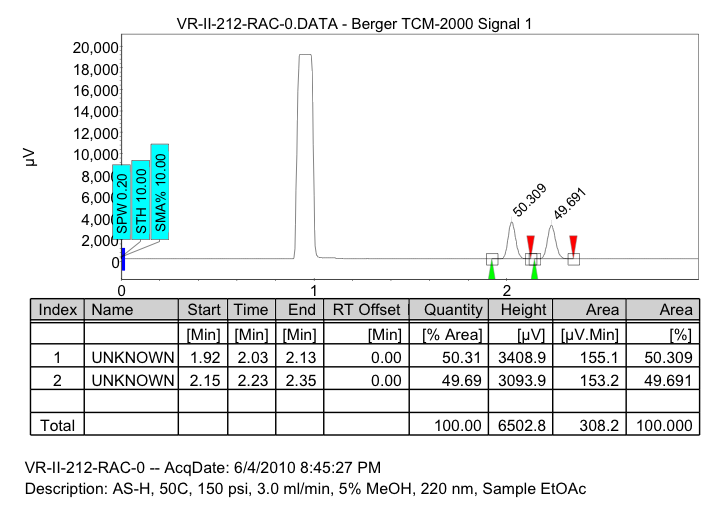
\includegraphics[width=2.75in]{chp_asymmetric/images/sfc/xaas-rac.png}
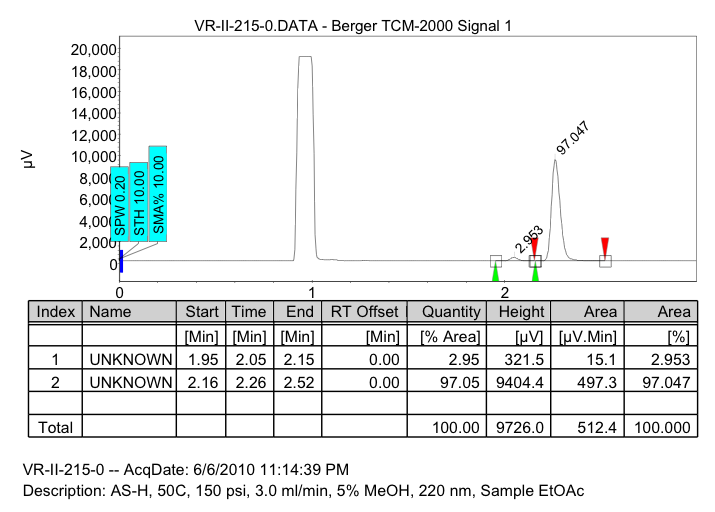
\includegraphics[width=2.75in]{chp_asymmetric/images/sfc/xaas.png}
\caption{SFC trace for \CMPxaas~(\ref{cmp:xaas})}
\vspace{-10pt}
\end{figure}
%***************[xaas]%***************%

\pagebreak
%***************[xaat]%***************%
\begin{wrapfigure}{l}{1.15in}
  \vspace{-12pt}
  \begin{center}
    
\includegraphics[scale=0.8]{chp_asymmetric/images/xaat}
  \end{center}
  \vspace{-25pt}
\end{wrapfigure}\noindent \textbf{\CMPxaat}\ (\ref{cmp:xaat}). Run for 14 hours
at $-$78 \degc\  according to the representative procedure with scandium
triflate (7.4 mg, 0.015 mmol, 10 mol \%), ligand \ref{cmp:ligandaa} (5.9 mg, 0.016 mmol, 11
mol \%), toluene (1.5 mL), cycloheptanone (18 $\mu$L, 0.15 mmol, 1.0 equiv), and
\ref{cmp:diazoaf} (180 $\mu$L, 0.21 mmol, 1.2 M in toluene, 1.4 equiv). The
crude reaction mixture was directly purified by column chromatography to afford
\ref{cmp:xaat} as a colorless oil (31.3 mg, 96.6\%) with 93.5:6.5 er (AS-H, 50
\degc, 150 psi, 2.5 mL/min, 2\% MeOH, $\lambda$ = 220 nm; t$_R$ = 2.74 min
(minor), 3.11 min (major)). \\
\rotation = $-$98.1 (c 1.26, CHCl$_3$); R$_f$ = 0.21 (10\% ethyl acetate in
hexanes); $^1$H NMR (CDCl$_3$, 400 MHz) $\delta$ 7.45-7.41 (m, 1H), 7.23-7.17
(m, 1H), 7.16-7.10 (m, 2H), 4.06 (dd, \textit{J} = 12.1, 2.7 Hz, 1H), 2.72 (ddd,
\textit{J} = 13.1, 11.7, 4.3 Hz, 1H), 2.46-2.35 (m, 1H), 2.40 (s, 3H), 2.33-2.23
(m, 1H), 2.01- 1.87 (m, 3H), 1.84-1.71 (m, 2H), 1.67-1.46 (m, 4H); $^{13}$C NMR
(CDCl$_3$, 100	MHz) $\delta$ 216.22,	138.06,	136.47, 130.63, 127.04, 126.83,
126.33, 53.04, 40.77, 32.02, 27.21, 27.15, 27.04, 24.91, 20.21; IR (neat) 3096
(w), 3020 (w), 2927 (bs), 2856 (w), 1697 (s), 1488 (w), 1464 (m), 1446 (m), 1325
(m), 1160 (w), 1123 (w), 845 (w), 755 (bm), 730 (m) cm$^{-1}$; HRMS (ESI+)
Calcd. for \ce{C15H21O} [M+H]$^+$: 217.1591; Found: 217.1592.  \\
\begin{figure}[h]
\centering
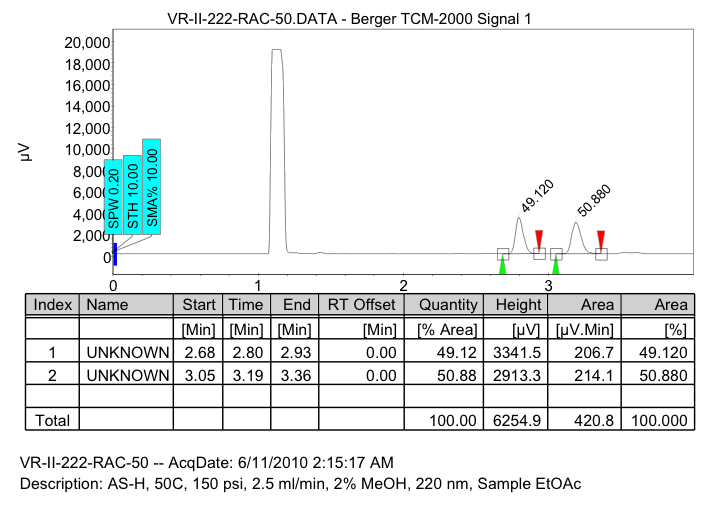
\includegraphics[width=2.75in]{chp_asymmetric/images/sfc/xaat-rac.png}
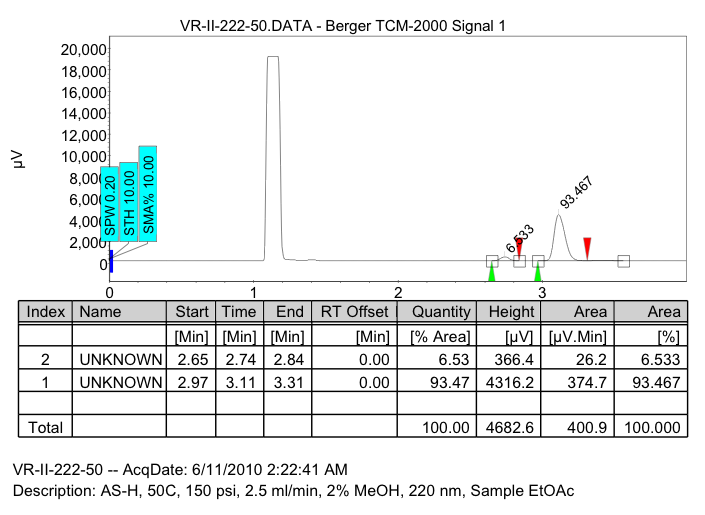
\includegraphics[width=2.75in]{chp_asymmetric/images/sfc/xaat.png}
\caption{SFC trace for \CMPxaat~(\ref{cmp:xaat})}
\vspace{-10pt}
\end{figure}
%***************[xaat]%***************%

\pagebreak
%***************[xaau]%***************%
\begin{wrapfigure}{l}{1.4in}
  \vspace{-12pt}
  \begin{center}
    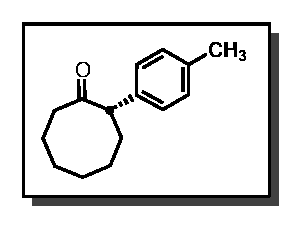
\includegraphics[scale=0.8]{chp_asymmetric/images/xaau}
  \end{center}
  \vspace{-25pt}
\end{wrapfigure}\noindent \textbf{\CMPxaau}\ (\ref{cmp:xaau}). Run for 3 hours
at $-$78 \degc\  according to the representative procedure with scandium
triflate (7.4 mg, 0.015 mmol, 10 mol \%), ligand \ref{cmp:ligandab} (8.5 mg,
0.016 mmol, 11 mol \%), toluene (1.5 mL), cycloheptanone (18 $\mu$L, 0.15 mmol,
1.0 equiv), and \ref{cmp:diazoah} (320 $\mu$L, 0.21 mmol, 0.66 M in toluene, 1.4
equiv). The crude reaction mixture was directly purified by column
chromatography to afford \ref{cmp:xaau} as a colorless oil (32.5 mg,
quantitative) with 98.5:1.5 er (AS-H, 50 \degc, 150 psi, 3.0 mL/min, 4\% MeOH,
$\lambda$ = 220 nm; t$_R$ = 1.90 min (minor), 2.13 min (major)).\\
\rotation = $-$148.9 (c 0.98, CHCl$_3$); R$_f$ = 0.37 (10\% ethyl acetate in
hexanes); $^1$H NMR (CDCl$_3$, 400 MHz) $\delta$ 7.22 (d, \textit{J} = 8.2 Hz,
2H), 7.11 (d, \textit{J} = 8.0 Hz, 2H), 3.74 (dd, \textit{J} = 12.3, 2.7 Hz,
1H), 2.61 (ddd, \textit{J} = 12.7, 11.7, 4.5 Hz, 1H), 2.42-2.29 (m, 1H), 2.31
(s, 3H), 2.26- 2.20 (m, 1H), 2.00-1.85 (m, 3H), 1.81-1.70 (m, 2H), 1.63-1.54 (m,
2H), 1.53-1.36 (m, 2H); $^{13}$C NMR (CDCl$_3$, 100	MHz) $\delta$ 216.75,
136.78, 136.44, 129.37,	127.76, 57.26, 40.16, 31.46, 27.13, 26.92, 26.82, 24.78,
21.13; IR (neat) 3021 (bw), 2926 (bs), 2856 (bm), 1698 (s), 1513 (m), 1465 (w),
1446 (w), 1159 (w), 818 (m) cm$^{-1}$; HRMS (ESI+) Calcd. for \ce{C15H21O}
[M+H]$^+$: 217.1592; Found: 217.1599.  \\
\begin{figure}[h]
\centering
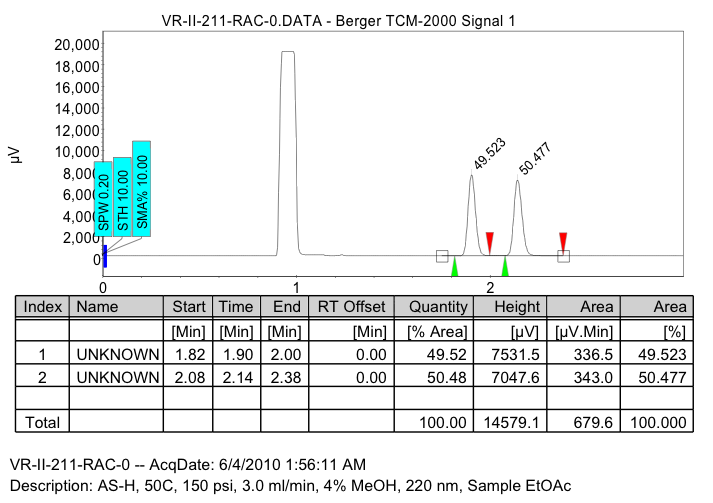
\includegraphics[width=2.75in]{chp_asymmetric/images/sfc/xaau-rac.png}
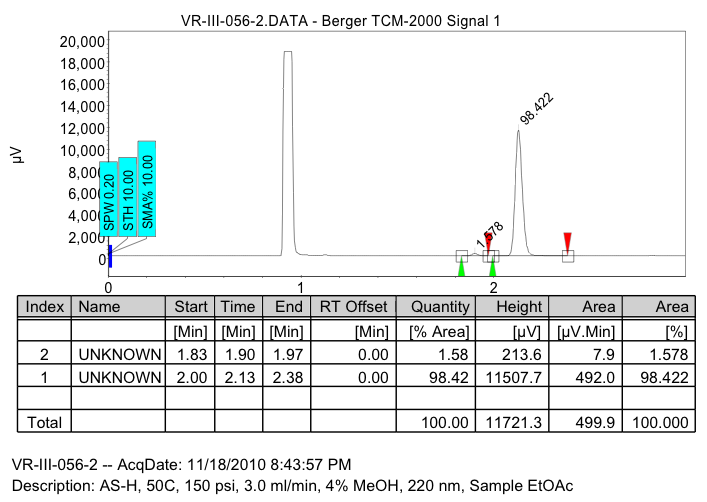
\includegraphics[width=2.75in]{chp_asymmetric/images/sfc/xaau.png}
\caption{SFC trace for \CMPxaau~(\ref{cmp:xaau})}
\vspace{-10pt}
\end{figure}
%***************[xaau]%***************%

\pagebreak
%***************[xaav]%***************%
\begin{wrapfigure}{l}{1.3in}
  \vspace{-12pt}
  \begin{center}
    
\includegraphics[scale=0.8]{chp_asymmetric/images/xaav}
  \end{center}
  \vspace{-25pt}
\end{wrapfigure}\noindent \textbf{\CMPxaav}\ (\ref{cmp:xaav}). Run for 14 hours
at $-$78 \degc\  according to the representative procedure with scandium
triflate (7.4 mg, 0.015 mmol, 10 mol \%), ligand \ref{cmp:ligandaa} (5.9 mg, 0.016
mmol, 11 mol \%), toluene (1.5 mL), cycloheptanone (18 $\mu$L, 0.15 mmol, 1.0
equiv), and \ref{cmp:diazoag} (396 $\mu$L, 0.21 mmol, 0.53 M in toluene, 1.4
equiv). The crude reaction mixture was directly purified by column
chromatography to afford \ref{cmp:xaav} as a pale yellow solid (35.5 mg, 93.9\%)
with 93:7 er (AD-H, 50 \degc, 150 psi, 2.0 mL/min, 3\% MeOH, $\lambda$ = 220 nm;
t$_R$ = 21.52 min (major), 25.15 min (minor)). mp 97- 100 \degc. \\
\rotation = +48.3 (c 0.82, CHCl$_3$); R$_f$ = 0.20 (10\% ethyl acetate in
hexanes); $^1$H NMR (CDCl$_3$, 400 MHz) $\delta$ 8.33-8.28 (m, 1H), 7.87-7.83
(m, 1H), 7.79-7.74 (m, 1H), 7.64-7.60 (m, 1H), 7.60-7.54 (m, 1H), 7.51-7.45 (m,
2H), 4.65 (dd, \textit{J} =  12.1, 2.6 Hz, 1H), 2.82 (ddd, \textit{J} =  12.3,
12.3, 3.9 Hz, 1H), 2.68-2.55 (m, 1H), 2.30 (ddd, \textit{J} =  12.9, 5.7, 3.7
Hz, 1H), 2.11-1.94 (m, 3H), 1.90-1.79 (m, 2H), 1.78-1.63 (m, 2H), 1.61-1.49 (m,
2H); $^{13}$C NMR	(CDCl$_3$,	100	MHz) $\delta$ 215.91,	135.62,	134.07, 131.86,
129.01, 127.75, 126.46, 125.70, 125.59, 124.63, 123.68, 52.49, 39.88, 31.66,
27.41, 27.30, 26.91, 24.92; IR (neat) 3042 (w), 2924 (bm), 2898 (bw), 1689 (s),
1510 (w), 1397 (w), 1117 (m), 800 (m), 780 (bs) cm$^{-1}$; HRMS (ESI+) Calcd.
for \ce{C18H21O} [M+H]$^+$: 253.1592; Found: 253.1622.  \\
\begin{figure}[h]
\centering
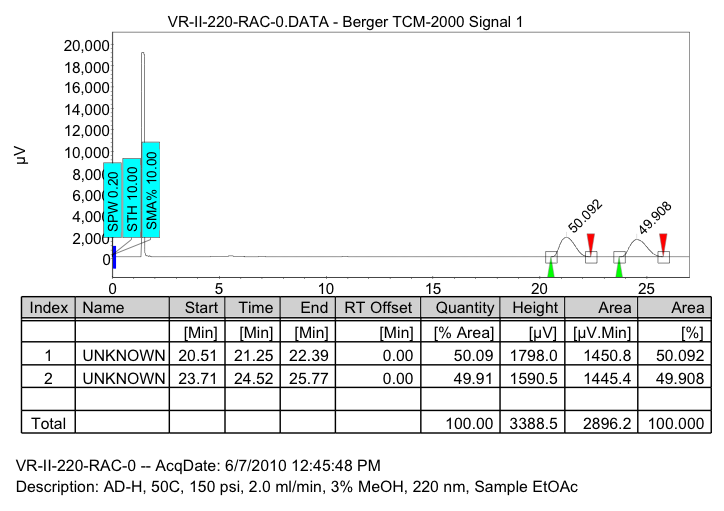
\includegraphics[width=2.75in]{chp_asymmetric/images/sfc/xaav-rac.png}
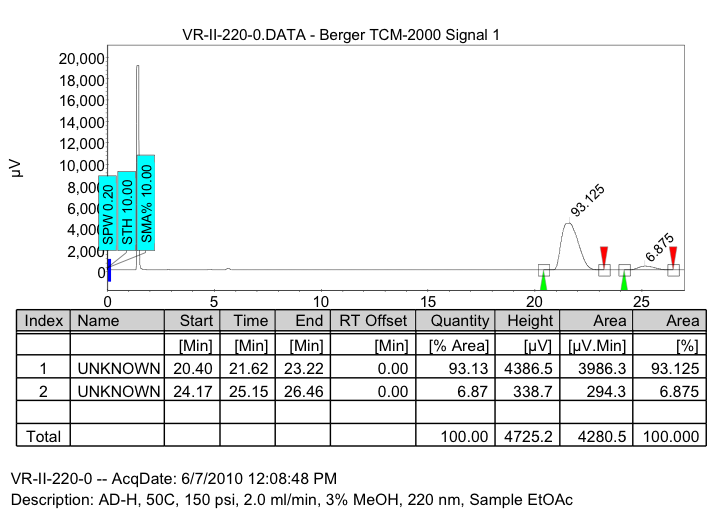
\includegraphics[width=2.75in]{chp_asymmetric/images/sfc/xaav.png}
\caption{SFC trace for \CMPxaav~(\ref{cmp:xaav})}
\vspace{-10pt}
\end{figure}
%***************[xaav]%***************%

\pagebreak
%***************[xaaw]%***************%
\begin{wrapfigure}{l}{1.35in}
  \vspace{-23pt}
  \begin{center}
    
\includegraphics[scale=0.8]{chp_asymmetric/images/xaaw}
  \end{center}
  \vspace{-30pt}
\end{wrapfigure}\noindent \textbf{\CMPxaaw}\ (\ref{cmp:xaaw}). Run for 14 hours
at $-$45 \degc\  according to the general procedure with scandium triflate (7.4
mg, 0.015 mmol, 10 mol \%), ligand \ref{cmp:ligandab} (8.5 mg, 0.016 mmol, 11
mol \%), toluene (1.5 mL), cyclooctanone (18.9 mg, 0.15 mmol, 1.0 equiv) in 0.15
mL of toluene, and \ref{cmp:diazoaa} (284 $\mu$L, 0.21 mmol, 0.74 M in toluene,
1.4 equiv). The crude reaction mixture was directly purified by column
chromatography to afford \ref{cmp:xaaw} as a colorless oil (33.0 mg,
quantitative) with 93:7 er (AD-H, 50 \degc, 150 psi, 2.0 mL/min, 2\% MeOH,
$\lambda$ = 220 nm; t$_R$ = 9.04 min (minor), 9.82 min (major)).\\
\rotation = $-$43.9 (c 0.94, CHCl$_3$); R$_f$ = 0.25 (10\% ethyl acetate in
hexanes); $^1$H NMR (CDCl$_3$, 400 MHz) $\delta$ 7.29- 7.14 (m, 5H), 3.88 (dd,
\textit{J} = 11.9, 2.7 Hz, 1H), 2.46-2.34 (m, 1H), 2.34-2.24 (m, 2H), 1.95-1.34
(m, 11H); $^{13}$C NMR (CDCl$_3$, 100 MHz) $\delta$ 216.28, 139.72, 128.68,
128.02, 127.12, 58.94, 41.80, 31.78, 25.97, 25.68, 25.49, 24.22, 24.02; IR
(neat) 3061 (bw), 3026 (bw), 2926 (bm), 1702 (s), 1495 (w), 1451 (m), 698 (s)
cm$^{-1}$; HRMS (ESI+) Calcd. for \ce{C15H21O} [M+H]$^+$: 217.1592; Found:
217.1589.
\\
\begin{figure}[h]
\centering
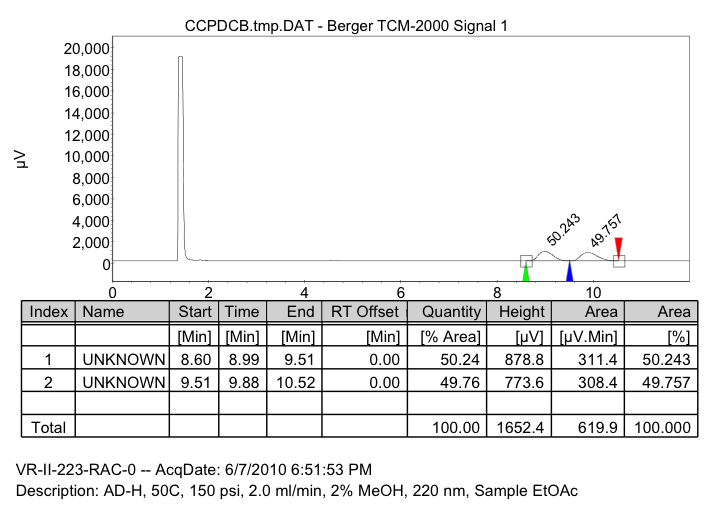
\includegraphics[width=2.75in]{chp_asymmetric/images/sfc/xaaw-rac.png}
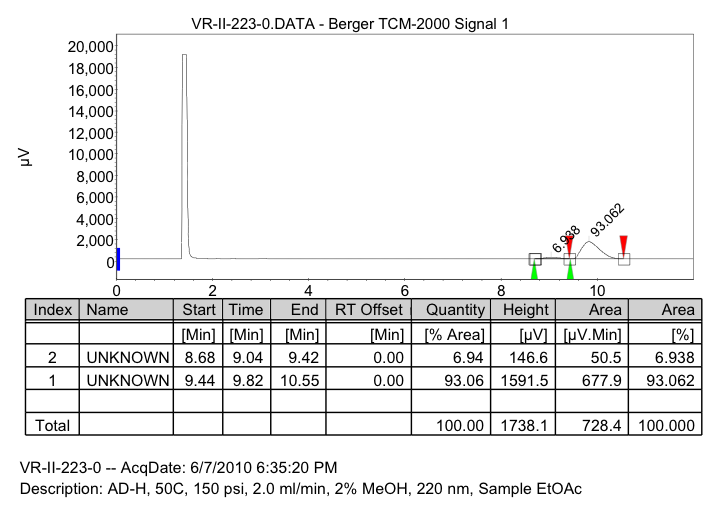
\includegraphics[width=2.75in]{chp_asymmetric/images/sfc/xaaw.png}
\caption{SFC trace for \CMPxaaw~(\ref{cmp:xaaw})}
\vspace{-10pt}
\end{figure}
%***************[xaaw]%***************%

\pagebreak
%***************[xaay]%***************%
\begin{wrapfigure}{l}{1.45in}
  \vspace{-22pt}
  \begin{center}
    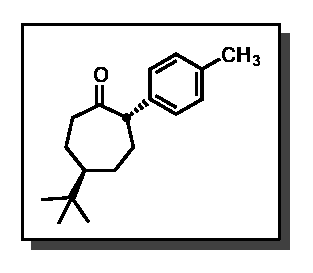
\includegraphics[scale=0.8]{chp_asymmetric/images/xaax}
  \end{center}
  \vspace{-30pt}
\end{wrapfigure}\noindent \textbf{\CMPxaay}\ (\ref{cmp:xaay}). Run for 3 hours
at $-$78 \degc\  on 0.15 mmol scale according to the representative procedure.
Purification by flash column chromatography (8\% ethyl acetate in hexanes v/v)
afforded the title compound as a white solid (31.0 mg, 79.9\%) with 92.5:7.5 er
(AS-H, 50 \degc, 150 psi, 3.0 mL/min, 4\% MeOH, $\lambda$ = 220 nm; t$_R$ = 1.98
min (minor), 3.05 min (major)). GC analysis of the crude reaction mixture showed
a 93:7 dr (HP-5, 150 \degc\ hold 5 min, ramp 5 \degc/min to 200 \degc; t$_R$ =
16.9 min (minor), 17.4 min (major)). Characterization data were in agreement with those tabulated above for the racemic compound. \rotation = $-$117.6 ($c$ 1.03, CHCl$_3$).
\\
\begin{figure}[h]
\centering
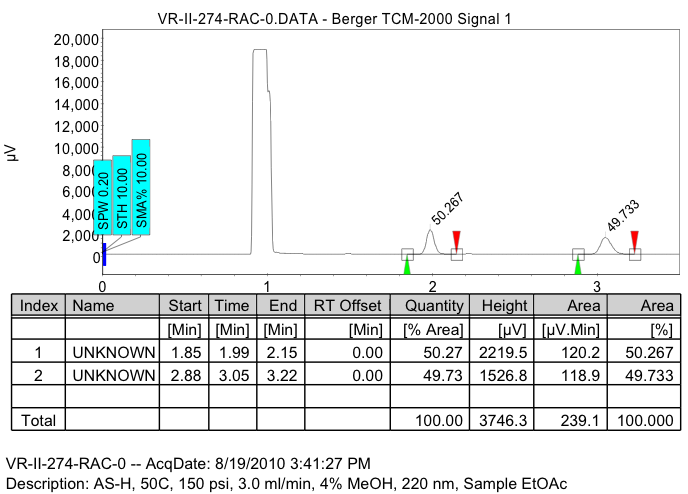
\includegraphics[width=2.75in]{chp_asymmetric/images/sfc/xaay-rac.png}
\includegraphics[width=2.75in]{chp_asymmetric/images/sfc/xaay.png}
\caption{SFC trace for \CMPxaay~(\ref{cmp:xaay})}
\vspace{-10pt}
\end{figure}
%***************[xaay]%***************%

\pagebreak
%***************[xaaz]%***************%
\begin{wrapfigure}{l}{1.45in}
  \vspace{-22pt}
  \begin{center}
    \includegraphics[scale=0.8]{chp_asymmetric/images/xaaz}
  \end{center}
  \vspace{-30pt}
\end{wrapfigure}\noindent \textbf{\CMPxaaz}\ (\ref{cmp:xaaz}).  To a stirred solution of
4-\textit{tert}-butylcyclohexanone (154 mg, 1.00 mmol) in 6.7 mL of CH$_2$Cl$_2$, trimethylaluminum
(0.27 mL, 0.55 mmol, 2.0 M in toluene) was added at $-$78 \degc. After stirring for an additional 5
minutes, \textit{p}-tolylphenyldiazomethane (0.76 mL, 0.50 mmol, 0.66 M in toluene) was introduced
in a single portion. After 30 minutes at $-$78 \degc, the reaction mixture was warmed to room
temperature and slowly quenched by dropwise addition of water. The solution was diluted with 10 mL
of water and extracted with CH$_2$Cl$_2$ (3 x 10 mL). The organic extracts were dried over anhydrous
Na$_2$SO$_4$ and concentrated to a crude yellow solid. Purification by preparative thin layer
chromatography (2.5\% ethyl acetate in hexanes v/v) afforded sufficient quantities of the minor
\textit{cis} diastereomer ($\pm$)-\ref{cmp:xaaz} for characterization. GC analysis of the crude
reaction mixture showed an 81.5:18.5 dr (HP-5, 150 \degc\ hold 5 min, ramp 5 \degc/min to 200 \degc;
t$_R$ = 16.9 min (minor), 17.4 min (major)).\\
$^1$H NMR (CDCl$_3$, 400 MHz) $\delta$ 7.14 (d, \textit{J} = 8.0 Hz, 2H), 7.08 (d, \textit{J} = 8.0
Hz, 2H), 3.77 (dd, \textit{J} = 5.9, 5.9 Hz, 1H), 2.73-2.65 (m, 1H), 2.62-2.53 (m, 1H), 2.32 (s,
3H), 2.30-2.21 (m, 1H), 2.14-2.06 (m, 1H), 2.01-1.89 (m, 2H), 1.48-1.32 (m, 3H), 0.87 (s, 9H);
$^{13}$C NMR (CDCl$_3$, 100 MHz) $\delta$ 213.64, 137.27, 136.46, 129.31, 128.24, 57.10, 49.56,
41.85, 33.73, 30.30, 27.63, 26.75, 25.14, 21.18; IR (neat) 2953 (bs), 2926 (bs), 2864 (bm), 1705
(m), 1514 (w), 1467 (bw), 1454 (bw), 1367 (w), 803(w)  cm$^{-1}$; HRMS (ESI+) Calcd. for
C$_{18}$H$_{27}$O [M+H]$^+$: 259.2062; Found: 259.2074.
% ***************[xaaz]%***************%

\vspace{10pt}
%***************[xaba]%***************%
% %% numbered as racemic xabc
\begin{wrapfigure}{l}{1.05in}
  \vspace{-20pt}
  \begin{center}
    \includegraphics[scale=0.8]{chp_asymmetric/images/xaba}
  \end{center}
  \vspace{-25pt}
\end{wrapfigure}\noindent \textbf{\CMPxaba}\ (\ref{cmp:xabc}). To a stirred solution of ketone
\ref{cmp:xaaj} (202 mg, 1.00 mmol) in 2.0 mL of THF, K-selectride (5.0 mL, 5.0 mmol, 1.0 M in THF)
was added dropwise at $-$78 \degc.
The reaction mixture was allowed to slowly warm to room temperature. After 24 hours, the pale yellow
solution was cooled to 0 \degc\ and quenched by adding 500 $\mu$L of water followed by 6.0 mL of 3N
aqueous NaOH. While stirring vigorously, 6.0 mL of 35\% H$_2$O$_2$  was added dropwise carefully.
The reaction mixture was warmed to room temperature an allowed to stir for an additional 3 hours.
The aqueous layer was extracted 3 times with 20 mL of Et$_2$O, washed with 50 mL of brine, and dried
over anhydrous Na$_2$SO$_4$. Concentration afforded a crude colorless oil that was purified by flash
column chromatography (18\% ethyl acetate in hexanes) to afford the desired product
($\pm$)-\ref{cmp:xabc} as a colorless oil (148 mg, 72.5\%, 98.2\% brsm) along with the starting
ketone (52.8 mg, 26.1\%). $^1$H NMR analysis of the crude reaction mixture showed $>$98:2 diastereoselectivity.\\
R$_f$ = 0.32 (20\% ethyl acetate in hexanes); $^1$H NMR (CDCl$_3$, 400 MHz) $\delta$ 7.36-7.31 (m,
2H), 7.29-7.20 (m, 3H), 3.91-3.86 (m, 1H), 3.07 (ddd, \textit{J} = 10.2, 2.7, 2.7 Hz, 1H), 2.28-2.17
(m, 1H), 1.89-1.73 (m, 5H), 1.73-1.54 (m, 6H), 1.32 (s, 1H); $^{13}$C NMR (CDCl$_3$, 100 MHz)
$\delta$ 145.35, 128.65, 126.51, 74.04, 47.95, 32.25, 27.98, 27.65, 27.65, 27.08, 26.07, 22.56; IR
(neat) 3431 (bm), 3025 (w), 2918 (bs), 2857 (bm), 1492 (w), 1471 (m), 1031 (m), 749 (m), 701 (s)
cm$^{-1}$; HRMS (ESI+) Calcd. for C$_{14}$H$_{24}$NO [M+NH$_4$]$^+$: 222.1858; Found: 222.1865.
% ***************[xaba]%***************%

\vspace{10pt}
%***************[xabb]%***************%
\begin{wrapfigure}{l}{1.6in}
  \vspace{-25pt}
  \begin{center}
    \includegraphics[scale=0.8]{chp_asymmetric/images/xabb}
        \begin{textblock}{1}(0.4,-1) \cmp{xabb} \end{textblock}
  \end{center}
  \vspace{-30pt}
\end{wrapfigure}\noindent \textbf{\CMPxabb}\ (\ref{cmp:xabb}). To a solution of
($\pm$)-\ref{cmp:xabc} (145 mg, 0.71 mmol) in
3.5 mL of CH$_2$Cl$_2$, DMAP (8.6 mg, 0.071 mmol) and Et$_3$N (148 $\mu$L, 1.06
mmol) were added. The solution was cooled to 0 \degc\ and 4-nitrobenzoyl
chloride (197 mg, 1.06 mmol) was added in a single portion. The reaction was
allowed to warm to room temperature and stirred on for 12 hours. The yellow
suspension was diluted with 25 mL of CH$_2$Cl$_2$, washed with 15 mL of 1 N HCl
and then dried over anhydrous Na$_2$SO$_4$. Concentration afforded a crude
yellow solid that was purified by flash column chromatography (15\% ethyl
acetate in hexanes v/v) to afford the title compound as a white solid (231.8 mg,
92.6\%). mp 93-94 \degc. Suitable crystals for X-ray analysis were grown by slow
evaporation from a 5\% (v/v) solution of Et$_2$O in hexanes.\\
R$_f$ = 0.47 (20\% ethyl acetate in hexanes); $^1$H NMR (CDCl$_3$, 400 MHz)
$\delta$ 8.29 (d, \textit{J} = 9.0 Hz, 2H), 8.10 (d, \textit{J} = 8.8 Hz, 2H),
7.31-7.26 (m, 4H), 7.24-7.19 (m, 1H), 5.54 (ddd, \textit{J} = 9.6, 3.7, 3.7 Hz,
1H), 3.31 (ddd, \textit{J} = 10.8, 3.3, 3.3 Hz, 1H), 2.43-2.32 (m, 1H),
2.18-2.08 (m, 1H), 2.06-1.70 (m, 10H); $^{13}$C NMR (CDCl$_3$, 100 MHz) $\delta$
163.83, 150.51, 143.94, 136.31, 130.65, 128.54, 128.30, 126.63, 123.59, 78.04,
46.70, 29.95, 28.99, 27.25, 26.96, 26.83, 23.41; IR (neat) 3028 (bw), 2926 (bm),
2858 (bw), 1719 (s), 1607 (w), 1527 (s), 1347 (m), 1274 (s), 1118 (m), 1102 (m),
719 (m), 702 (m) cm$^{-1}$; HRMS (ESI+) Calcd. for C$_{21}$H$_{27}$N$_{2}$O$_{4}$ [M+NH$_4$]$^+$: 371.1971; Found: 371.1979.
%***************[xabb]%***************%

\vspace{10pt}
%***************[xabc]%***************%
\begin{wrapfigure}{l}{1.05in}
  \vspace{-22pt}
  \begin{center}
    \includegraphics[scale=0.8]{chp_asymmetric/images/xaba}
  \end{center}
  \vspace{-25pt}
\end{wrapfigure}\noindent \textbf{\CMPxabc}\ (\ref{cmp:xabc}). To a stirred
solution of ketone \ref{cmp:xaal} (102 mg, 0.50 mmol) in 5.4 mL of toluene,
Red-Al (747 $\mu$L, 2.45 mmol, 65\% w/w in toluene) was added \textit{via}
syringe pump over 30 minutes at $-$78 \degc. The reaction mixture was allowed to
warm to room temperature slowly and stirred for an additional 16 hours. The
clear solution was cooled to 0 \degc\ and quenched with water until evolution of
hydrogen gas ceased. The entire reaction mixture was poured into 15 mL of 1 N
HCl and extracted three times with 15 mL of Et$_2$O. The organic extracts were
dried over anhydrous Na$_2$SO$_4$ and concentrated to deliver a crude colorless
oil. Purification by flash column chromatography (18\% ethyl acetate in hexanes
v/v) afforded the desired product as a colorless oil (68.6 mg, 66.3\%). $^1$H
NMR analysis of the crude reaction mixture showed a 2.5:1 mixture of \textit{cis} to
\textit{trans} diastereomers. Characterization data were identical to that
reported above for the racemic material.
%***************[xabc]%***************%

\vspace{10pt}
%***************[xabd]%***************%
\begin{wrapfigure}{l}{1.35in}
  \vspace{-22pt}
  \begin{center}
    \includegraphics[scale=0.8]{chp_asymmetric/images/xabd}
  \end{center}
  \vspace{-25pt}
\end{wrapfigure}\noindent \textbf{\CMPxabd}\ (\ref{cmp:xabd}). A 1-dram vial was
charged with (1\textit{S},2\textit{S})-2-phenylcyclooctanol \ref{cmp:xabc} (16
mg, 0.078 mmol), (\textit{S})-$\alpha$-acetylmandelic acid (17 mg, 0.086 mmol),
\ce{EDC.HCl} (18 mg, 0.094 mmol), and DMAP (4.8 mg, 0.039 mmol). Bench-top
CH$_2$Cl$_2$ (1.0 mL) was added followed by triethylamine (13 $\mu$L, 0.094
mmol). The vial was sealed with a screw-cap and stirred for 18 hours. The
reaction was quenched with 1 mL of water. The aqueous layer was removed and the
remaining organics were washed with 1 mL of saturated NaHCO$_3$, 1 mL of brine,
and finally dried over anhydrous Na$_2$SO$_4$. Purification directly by preparative thin layer chromatography (15\% ethyl acetate in hexanes v/v) afforded sufficient quantities of the title compound for NMR analysis.\\
$^1$H NMR (CDCl$_3$, 500 MHz) $\delta$ 7.44-7.35 (m, 5H), 7.05-7.01 (m, 1H),
6.97-6.93 (m, 2H), 6.73-6.70 (m, 2H), 5.85 (s, 1H), 5.24-5.20 (m, 1H), 2.96
(ddd, \textit{J} = 10.5, 2.9, 2.9 Hz, 1H), 2.14 (s, 3H), 2.10-2.01 (m, 1H),
1.99-1.91 (m, 1H), 1.90-1.83 (m, 1H), 1.82-1.73 (m, 2H), 1.72-1.57 (m, 7H);
$^{13}$C NMR (CDCl$_3$, 125 MHz) $\delta$ 170.43, 168.06, 143.95, 134.11,
129.29, 128.89, 128.23, 128.11, 128.07, 126.07, 77.93, 74.91, 46.01, 30.31,
29.22, 27.65, 26.81, 26.52, 22.82, 20.88; IR (neat) 2922 (bw), 2859 (bw), 1739 (s), 1453 (w), 1371 (m), 1230 (s), 1209 (s), 1177 (s), 1051 (bm), 750 (m), 695 (m) cm$^{-1}$; HRMS (ESI+) Calcd. for C$_{24}$H$_{32}$NO$_4$ [M+NH$_4$]$^+$: 398.2331; Found: 398.2330.
%***************[xabd]%***************%

\vspace{10pt}
%***************[xabe]%***************%
\begin{wrapfigure}{l}{1.35in}
  \vspace{-22pt}
  \begin{center}
    \includegraphics[scale=0.8]{chp_asymmetric/images/xabe}
  \end{center}
  \vspace{-25pt}
\end{wrapfigure}\noindent \textbf{\CMPxabe}\ (\ref{cmp:xabe}). Prepared in an
analogous fashion to the diastereomer above (\ref{cmp:xabd}) with
(\textit{R})-$\alpha$-acetylmandelic acid. The following characterization data
were obtained: \\
$^1$H NMR (CDCl$_3$, 500 MHz) $\delta$ 7.41-7.36 (m, 1H), 7.35-7.33 (m, 4H),
7.28-7.24 (m, 2H), 7.21-7.17 (m, 3H), 5.86 (s, 1H), 5.22 (ddd, \textit{J} = 9.0,
3.7, 3.7 Hz, 1H), 3.10 (ddd, \textit{J} = 10.8, 3.4, 3.4 Hz, 1H), 2.14 (s, 3H), 2.13-2.08 (m, 1H), 1.87-1.80 (m, 1H), 1.79-1.70 (m, 2H), 1.70-1.49 (m, 8H); $^{13}$C NMR (CDCl$_3$, 125 MHz) $\delta$ 170.24, 168.11, 144.04, 134.23, 129.08, 128.75, 128.62, 128.28, 127.61, 126.44, 77.69, 74.74, 46.44, 29.75, 29.35, 27.18, 26.88, 26.53, 22.83, 20.83; IR (neat) 2921 (bm), 2853 (bw), 1739 (s), 1452 (w), 1371 (m), 1228 (s), 1209 (s), 1176 (s), 1051 (bm), 967 (bw), 750 (m), 694 (m) cm$^{-1}$; HRMS (ESI+) Calcd. for C$_{24}$H$_{32}$NO$_4$ [M+NH$_4$]$^+$: 398.2331; Found: 398.2339.
%***************[xabe]%***************%

\pagebreak
% ***************[diazoaa]%***************%
\begin{wrapfigure}{l}{0.95in}
  \vspace{-10pt}
  \begin{center}
    \includegraphics[scale=0.8]{chp_asymmetric/images/diazoaa}
  \end{center}
  \vspace{-30pt}
\end{wrapfigure}\noindent \textit{Representative procedure for preparation of
aryl diazoalkanes:} \\ \textbf{\CMPdiazoaa}\ (\ref{cmp:diazoaa}).
Benzaldehyde (1.05 g, 9.89 mmol) was weighed directly into a pressure tube then
stirred vigorously while hydrazine hydrate (4 mL) was added slowly. The pressure
tube was sealed and heated to 90 \degc \ for 12 hours. The reaction mixture was
poured into 10 mL of brine, extracted with CH$_2$Cl$_2$ (3 x 10 mL), dried over
anhydrous Na$_2$SO$_4$ and concentrated to a colorless oil in a 250 mL round
bottom flask. The crude hydrazone was flushed with argon and kept cold ($-$20
\degc) until use in the oxidation step. In a separate flask, dimethyl sulfoxide
(780 $\mu$L, 10.9 mmol, 1.10 equiv) in 10 mL of CH$_2$Cl$_2$ was cooled to $-$78
\degc\  and oxalyl chloride (910 $\mu$L, 10.4 mmol, 1.05 equiv) was added
dropwise \textit{via} syringe pump over 15 minutes. The oxidant solution was
stirred for an additional 15 minutes. During this time, the crude hydrazone was
dissolved in 90 mL of Et$_2$O, cooled to $-$78 \degc\ and triethylamine (2.9 mL,
20.8 mmol, 2.1 equiv) was added to the stirred solution. The oxidant, kept cold
at $-$78 \degc, was transferred \textit{via} cannula to the solution of
hydrazone and triethylamine which immediately formed a pink solution. After 45
minutes the reaction mixture was quickly extracted in a separatory funnel with
ice cold 50\% aq. NH$_4$Cl (100 mL), H$_2$O (100 mL), and saturated NaHCO$_3$.
The organics were dried by rapidly swirling over K$_2$CO$_3$ on an ice bath for
1 minute. The clear red solution was filtered through a sintered glass funnel
and then immediately concentrated under high vacuum (0.1 mm Hg) on a brine/ice
bath to yield the title compound as a red oil. The resulting oil was cooled to
$-$78 \degc\ and transferred to a 10 mL volumetric flask with toluene. If the
diazo solution was turbid or cloudy it was gravity filtered through a cotton
plug in a cold jacketed dropping funnel held at $-$78 \degc. The clear toluene
solution was stored over 3\AA\ sieves (4-8 mesh) at $-$78 \degc\ and titrated
with 2-fluorobenzoic acid according the the procedure below to give a
concentration of 0.74 M (0.87 g, 7.4 mmol, 75\%
yield).\footnote{Characterization data were obtained from the 2-fluorobenzoate
esters for each diazoalkane due to the hazards associated with handling neat
diazo compounds.}

\noindent \textit{Note:} The above procedure was applicable to all
aryl diazoalkanes prepared in this study except \ref{cmp:diazoag}. The
1-naphthyl hydrazone was sparingly soluble in Et$_2$O, thus resulting in low conversion to the
diazoalkane. Running the entire procedure in CH$_2$Cl$_2$ facilitated smooth and
complete conversion of the hydrazone.
% ***************[diazoaa]%***************%

\vspace{10pt}
%***************[xtaaa]%***************%
\begin{wrapfigure}{l}{1.45in}
  \vspace{-32pt}
  \begin{center}
    \includegraphics[scale=0.8]{chp_asymmetric/images/xtaaa}
    \begin{textblock}{1}(0.5,-2.65) \cmp{xtaaa} \end{textblock}
  \end{center}
  \vspace{-35pt}
\end{wrapfigure}\noindent \textit{Representative procedure for titration of
diazoalkane solutions:}\\ \textbf{\CMPxtaaa}\ (\ref{cmp:xtaaa}). A stock
solution of 2-fluorobenzoic acid in CDCl$_3$ was prepared by weighing 1.2591
grams directly into a 25.00 mL volumetric flask. The flask was diluted to the total
volume with CDCl$_3$, affording a 0.3595 M solution. The stock solution was
sealed with a ground glass stopper and stored in the
dark.\footnote{Alternatively, an accurately weighed sample of 2-fluorobenzoic
acid could be used. We have found that 2-fluorobenzoic acid dissolves slowly in
chloroform and therefore preparing a stock solution was generally more
convenient.} In an oven-dried 1-dram glass vial, the 2-fluorobenzoic acid
solution (700 $\mu$L, 0.252 mmol, 0.359 M in CDCl$_3$, excess) was added and
cooled to $-$78 \degc, causing the solution to freeze. A
100 $\mu$L aliquot of phenyldiazomethane (\ref{cmp:diazoaa}) in toluene was
added in a single portion, and the reaction was allowed to warm to room temperature. Upon reaching
room temperature, the reaction was complete as judged by the absence of color
and gas evolution. Approximately 5 $\mu$L of hexafluorobenzene was added as an
internal standard for spectrum calibration. The homogeneous colorless solution was transferred
\textit{via} glass pipette to an NMR tube for analysis. $^{19}$F NMR data (8 scans) were recorded
with a relaxation delay time of 10 seconds (d1 = 10), and integration of the two signals ($\delta$ = $-$111
acid, $\delta$ = $-$112 ester) showed the aliquot to contain 0.117 mmol of
diazoalkane based on 46.4\% conversion of the acid to the corresponding ester.
The procedure was repeated in triplicate to give a concentration value of 1.16
$\pm$ 0.03 M. The gravimetric benzoate ester method (see below for procedure)
gave a comparable concentration of 1.23 M. For characterization purposes, the
three samples from the $^{19}$F NMR titration procedure were transferred to a separatory funnel with 25 mL of Et$_2$O. The organic layer was washed with 1N NaOH (2 x 15 mL) and saturated NaCl (15 mL), dried over
\ce{Na2SO4}, filtered, and then concentrated. The product was purified by flash
column chromatography on silica gel (10\% ethyl acetate in hexanes v/v) to
afford the desired ester \ref{cmp:xtaaa} as a colorless oil.\\
\noindent R$_f$ = 0.36 (10\% ethyl acetate in hexanes); $^1$H NMR (CDCl$_3$, 500
MHz) $\delta$ 7.97 (ddd, \textit{J} =  7.6, 7.6, 1.7 Hz, 1H), 7.55-7.50 (m, 1H), 7.49-7.45
(m, 2H), 7.41-7.37 (m, 2H), 7.37-7.32 (m, 1H), 7.20 (ddd, \textit{J} =  7.6, 7.6, 1.0 Hz,
1H), 7.14 (ddd, \textit{J} =  10.8, 8.3, 1.0 Hz, 1H), 5.40 (s, 2H); $^{13}$C NMR
(CDCl$_3$, 125 MHz) $\delta$ 164.3 (d, \textit{J}$_{C\mbox{-}F}$ = 3.7 Hz), 162.2 (d, \textit{J}$_{C\mbox{-}F}$ = 260.5
Hz), 135.9, 134.7 (d, \textit{J}$_{C\mbox{-}F}$ = 9.3 Hz), 132.3 (d, \textit{J}$_{C\mbox{-}F}$ = 0.9 Hz), 128.7, 128.4,
128.2, 124.1 (d, \textit{J}$_{C\mbox{-}F}$ = 3.7 Hz), 118.8 (d, \textit{J}$_{C\mbox{-}F}$ = 9.8 Hz), 117.1 (d, \textit{J}$_{C\mbox{-}F}$ = 22.3
Hz), 67.0; $^{19}$F NMR (CDCl$_3$, 470 MHz) $\delta$ $-$112.26 (dddd,
\textit{J}$_{F\mbox{-}H}$ = 7.3, 7.3, 4.4, 4.4 Hz, 1F); IR (neat) 3066, 3034,
2954, 1714, 1612, 1488, 1455, 1292, 1247, 1120, 1075, 1030, 752, 693 cm$^{-1}$; HRMS (ESI+) Calcd. for
\ce{C14H12FO2} [M+H]$^+$: 231.0821; Found 231.0817.
\begin{singlespace}
\begin{table}[htbp]
\begin{textblock}{1}(0,1.3)
\includegraphics[scale=0.8]{chp_asymmetric/images/diazoaa}
\end{textblock}
\flushright
{\small
\begin{tabular}{ccccc} 
\toprule
&Ester&Acid&Percent&Diazoalkane\\
Trial&Integration&Integration&Conversion (\%)&Concentration (M) \\ 
\midrule
1 & 47.04 & 52.96 & 47.04 & 1.18$_4$ \\
2 & 46.42 & 53.58 & 46.42 & 1.16$_8$ \\
3 & 44.82 & 55.18 & 44.82 & 1.12$_8$ \\
\midrule
Stock & 0.3595 M & & Average & 1.16 \\
Solution & 0.252 mmol & & Std. Deviation & 0.03 \\
\bottomrule
\end{tabular}
\caption{Titration results for \CMPdiazoaa~(\ref{cmp:diazoaa})}
}
\end{table}
\end{singlespace}
\noindent \textit{General procedure for titration by isolation of the unpurified
benzoate ester:}
Benzoic acid (150 mg, 1.23 mmol, excess) was dissolved in 3 mL of \ce{CH2Cl2}
and cooled to $-$78 \degc. A 300 $\mu$L aliquot of the diazoalkane solution was
added in a single portion, and the reaction mixture was allowed to warm to room
temperature. After standing at room temperature for 30 minutes the reaction
mixture was transferred to a separatory funnel with 25 mL of Et$_2$O. The
organic layer was washed with 1N NaOH (2 x 15 mL) and saturated NaCl (15 mL),
dried over \ce{Na2SO4}, filtered, and then concentrated. The crude ester was
dried under high vacuum (approx. 1 mm Hg) for 12 hours and weighed to determine
yield. Analytically pure samples for new compounds were obtained by purification
on silica gel (ethyl acetate in hexanes). Characterization data for the
following benzoate esters have been reported previously:

\frenchspacing
\begin{itemize}
  \item \textbf{Methyl benzoate} Tobisu, M.; Yamakawa, K.; Shimasaki,
  T.; Chatani, N. \textit{Chem. Commun.} \textbf{2011}, \textit{47}, 2946-2948.
  \item \textbf{Benzyl benzoate} Tejel, C.; Ciriano, M. A.; Passarelli, V.
  \textit{Chem. Eur. J.} \textbf{2011}, \textit{17}, 91-95.
  \item \textbf{3-Phenylpropyl benzoate} Iranpoor, N.; Firouzabadi,
  H. Khalili, D.; Motevalli, S. \textit{J. Org. Chem.} \textbf{2008},
  \textit{73}, 4882-4887.
   \item \textbf{Cinnamyl benzoate, 1-Phenylethyl benzoate}
  Weng, S.; Ke, C.; Chen, F.; Lyu, Y.; Lin, G. \textit{Tetrahedron.}
  \textbf{2011}, \textit{67}, 1640-1648.
  \item \textbf{2-Methylbenzyl benzoate, 3-Methoxybenzyl benzoate}
  Iranpoor, N.; Firouzabadi, H.; Khalili, D. \textit{Org. Biomol. Chem.}
  \textbf{2010}, \textit{8}, 4436-4443.
  \item \textbf{4-Methylbenzyl benzoate} Kwok, M.; Choi, W.; He, H. S.;
  Toy, P. H. \textit{J. Org. Chem.} \textbf{2003}, \textit{68}, 9831-9834.
  \item \textbf{Naphthalen-1-ylmethyl benzoate} Kesharwani, T.;
  Larock, R. C. \textit{Tetrahedron.} \textbf{2008}, \textit{64}, 6090-6102.
  \item \textbf{Furan-2-ylmethyl benzoate} Chen, P.; Chou, C.
  \textit{Tetrahedron.} \textbf{1997}, \textit{53}, 17115-17126.
\end{itemize}
\nonfrenchspacing
% ***************[xtaaa]%***************%


\pagebreak
%***************[xtaab]%***************%
\begin{wrapfigure}{l}{1.1in}
  \vspace{-20pt}
  \begin{center}
    \includegraphics[scale=0.8]{chp_asymmetric/images/xtaab}
      \begin{textblock}{1}(0.5,-2.65) \cmp{xtaab} \end{textblock}
  \end{center}
  \vspace{-35pt}
\end{wrapfigure}\noindent \textbf{\CMPxtaab}\ (\ref{cmp:xtaab}). Prepared and
isolated according to the representative procedure for titration of diazoalkane
stock solutions. The fluorobenzoate ester method gave an average concentration
of 0.49 $\pm$ 0.05 M. The gravimetric benzoate ester method gave a concentration
of 0.34 M. colorless oil; R$_f$ = 0.28 (10\% ethyl acetate in hexanes); $^1$H
NMR (CDCl$_3$, 500 MHz) $\delta$ 7.94 (ddd, \textit{J} = 7.6, 7.6, 2.0 Hz, 1H),
7.54-7.49 (m, 1H), 7.21 (ddd, \textit{J} = 7.8, 7.8, 1.2 Hz, 1H), 7.14 (ddd,
\textit{J} = 11.0, 8.3, 1.2 Hz, 1H), 3.95 (s, 3H); $^{13}$C NMR (CDCl$_3$, 125
MHz) $\delta$ 164.9 (d, \textit{J}$_{C\mbox{-}F}$ = 3.7 Hz), 162.0 (d,
\textit{J}$_{C\mbox{-}F}$ = 259.6 Hz), 134.5 (d, \textit{J}$_{C\mbox{-}F}$ = 9.3
Hz), 132.2 (d, \textit{J}$_{C\mbox{-}F}$ = 0.9 Hz), 124.0 (d,
\textit{J}$_{C\mbox{-}F}$ = 4.2 Hz), 118.7 (d, \textit{J}$_{C\mbox{-}F}$ = 9.8
Hz), 117.0 (d, \textit{J}$_{C\mbox{-}F}$ = 22.3 Hz), 52.3; $^{19}$F NMR
(CDCl$_3$, 470 MHz) $\delta$ $-$112.73 (dddd, \textit{J}$_{F\mbox{-}H}$ = 5.5,
5.5, 5.5, 5.5 Hz, 1F); IR (neat) 3000, 2955, 1719, 1613, 1489, 1457, 1435, 1301,
1262, 1125, 1086, 756, 693 cm$^{-1}$; HRMS (ESI+) Calcd. for \ce{C8H8FO2}
[M+H]$^+$: 155.0508; Found 155.0513.

\begin{singlespace}
\begin{table}[htbp]
\begin{textblock}{1}(0,1.5)
\includegraphics[scale=0.8]{chp_asymmetric/images/diazoak}
\end{textblock}
\flushright
{\small
\begin{tabular}{ccccc} 
\toprule
&Ester&Acid&Percent&Diazoalkane\\
Trial&Integration&Integration&Conversion (\%)&Concentration (M) \\ 
\midrule
1 & 17.54 & 82.46 & 17.54 & 0.44$_1$ \\
2 & 21.43 & 78.57 & 21.43 & 0.53$_9$ \\
3 & 19.94 & 80.06 & 19.94 & 0.50$_2$ \\
\midrule
Stock & 0.3595 M & & Average & 0.49 \\
Solution & 0.252 mmol & & Std. Deviation & 0.05 \\
\bottomrule
\end{tabular}
\caption{Titration results for \CMPdiazoak~(\ref{cmp:diazoak})}
}
\end{table}
\end{singlespace}
% ***************[xtaab]%***************%

\pagebreak
%***************[xtaac]%***************%
\begin{wrapfigure}{l}{1.45in}
  \vspace{-15pt}
  \begin{center}
    \includegraphics[scale=0.8]{chp_asymmetric/images/xtaac}
          \begin{textblock}{1}(0.4,-2.6) \cmp{xtaac} \end{textblock}
  \end{center}
  \vspace{-35pt}
\end{wrapfigure}\noindent \textbf{\CMPxtaac}\ (\ref{cmp:xtaac}). Prepared and
isolated according to the representative procedure for titration of diazoalkane
stock solutions. The fluorobenzoate ester method gave an average concentration
of 0.133 $\pm$ 0.003 M. The gravimetric benzoate ester method gave a
concentration of 0.40 M. colorless oil; R$_f$ = 0.31 (10\% ethyl acetate in
hexanes); $^1$H NMR (CDCl$_3$, 500 MHz) $\delta$ 7.92 (ddd, \textit{J} = 7.6, 7.6, 1.7 Hz, 1H),
7.55-7.50 (m, 1H), 7.32-7.28 (m, 2H), 7.24-7.18 (m, 4H), 7.15 (ddd, \textit{J} =
11.0, 8.3, 1.0 Hz, 1H), 4.36 (t, \textit{J} = 6.4 Hz, 2H), 2.80 (t, \textit{J} =
7.3 Hz, 2H), 2.13-2.07 (m, 2H); $^{13}$C NMR (CDCl$_3$, 125 MHz) $\delta$ 164.6
(d, \textit{J}$_{C\mbox{-}F}$ = 3.6 Hz), 162.1 (d, \textit{J}$_{C\mbox{-}F}$ =
260.0 Hz), 141.3, 134.5 (d, \textit{J}$_{C\mbox{-}F}$ = 9.2 Hz), 132.2 (d,
\textit{J}$_{C\mbox{-}F}$ = 0.9 Hz), 128.6, 126.2, 124.1 (d, \textit{J}$_{C\mbox{-}F}$ = 4.1 Hz) 119.1 (d,
\textit{J}$_{C\mbox{-}F}$ = 9.7 Hz), 117.1 (d, \textit{J}$_{C\mbox{-}F}$ = 22.6
Hz), 64.7, 32.3, 30.4; $^{19}$F NMR (CDCl$_3$, 470 MHz) $\delta$ $-$112.49
(dddd, \textit{J}$_{F\mbox{-}H}$ = 6.6, 6.6, 4.4, 4.4 Hz, 1F); IR (neat) 3027, 2955,
2927, 1713, 1612, 1488, 1455, 1294, 1249, 1157, 1126, 1082, 1032, 754, 698
cm$^{-1}$; HRMS (ESI+) Calcd. for \ce{C16H16FO2} [M+H]$^+$: 259.1134; Found
259.1135.

\begin{singlespace}
\begin{table}[htbp]
\begin{textblock}{1}(0,1.5)
\includegraphics[scale=0.8]{chp_asymmetric/images/diazoal}
\end{textblock}
\flushright
{\small
\begin{tabular}{ccccc} 
\toprule
&Ester&Acid&Percent&Diazoalkane\\
Trial&Integration&Integration&Conversion (\%)&Concentration (M) \\ 
\midrule
1 & 5.27 & 94.73 & 5.27 & 0.132$_6$ \\
2 & 5.17 & 94.83 & 5.17 & 0.130$_1$ \\
3 & 5.43 & 94.57 & 5.43 & 0.136$_6$ \\
\midrule
Stock & 0.3595 M & & Average & 0.133\\
Solution & 0.252 mmol & & Std. Deviation & 0.003 \\
\bottomrule
\end{tabular}
\caption{Titration results for \CMPdiazoal~(\ref{cmp:diazoal})}
}
\end{table}
\end{singlespace}
% ***************[xtaac]%***************%

\pagebreak
%***************[xtaad]%***************%
\begin{wrapfigure}{l}{1.45in}
  \vspace{-15pt}
  \begin{center}
    \includegraphics[scale=0.8]{chp_asymmetric/images/xtaad}
          \begin{textblock}{1}(0.4,-2.6) \cmp{xtaad} \end{textblock}
  \end{center}
  \vspace{-35pt}
\end{wrapfigure}\noindent \textbf{\CMPxtaad}\ (\ref{cmp:xtaad}). Impurities present in the diazoalkane solution complicated the
isolation of \ref{cmp:xtaad}. An authentic sample for characterization was
prepared by Steglich esterification.\footnote{{\frenchspacing Neises, B.; Steglich, W. Simple Method
for the Esterification of Carboxylic Acids. \textit{Angew. Chem. Int. Ed.} \textbf{1978},
\textit{17}, 522-524.} \label{ref:steglich}} The fluorobenzoate ester method gave an average concentration of 0.43 $\pm$ 0.01 M. The gravimetric benzoate ester method gave a
concentration of 1.26 M. colorless oil; R$_f$ = 0.31 (10\% ethyl acetate in
hexanes); $^1$H NMR (CDCl$_3$, 500 MHz) $\delta$ 7.98 (ddd, \textit{J} = 7.6, 7.6, 1.7 Hz, 1H), 7.56-7.50 (m, 1H), 7.44-7.41 (m, 2H), 7.36-7.31 (m, 2H),
7.29-7.25 (m, 1H), 7.21 (ddd, \textit{J} = 7.6, 7.6, 1.2 Hz, 1H), 7.15 (ddd,
\textit{J} = 10.8, 8.3, 1.0 Hz, 1H), 6.77 (d, \textit{J} = 15.9 Hz, 1H), 6.41
(dt, \textit{J} = 15.9, 6.4 Hz, 1H), 5.01 (dd, \textit{J} = 6.4, 1.5 Hz, 2H);
$^{13}$C NMR (CDCl$_3$, 125 MHz) $\delta$ 164.1 (d, \textit{J}$_{C\mbox{-}F}$ =
3.6 Hz), 162.0 (d, \textit{J}$_{C\mbox{-}F}$ = 260.2 Hz), 136.2, 134.6 (d,
\textit{J}$_{C\mbox{-}F}$ = 8.7 Hz), 134.4, 132.2, 128.6, 128.1, 126.7, 124.0
(d, \textit{J}$_{C\mbox{-}F}$ = 3.6 Hz), 123.0, 118.8 (d,
\textit{J}$_{C\mbox{-}F}$ = 9.7 Hz), 117.0 (d, \textit{J}$_{C\mbox{-}F}$ = 22.5
Hz), 65.8; $^{19}$F NMR (CDCl$_3$, 470 MHz) $\delta$ $-$112.39 (dddd,
\textit{J}$_{F\mbox{-}H}$ = 7.3, 7.3, 5.1, 5.1 Hz, 1F); IR (neat) 3059, 3027,
2943, 1715, 1612, 1488, 1454, 1289, 1247, 1157, 1122, 1075, 1032, 964, 910, 754,
690 cm$^{-1}$; HRMS (ESI+) Calcd. for \ce{C16H17FNO2} [M+NH$_4$]$^+$: 274.1243;
Found 274.1231.

\begin{singlespace}
\begin{table}[htbp]
\begin{textblock}{1}(0,1.5)
\includegraphics[scale=0.8]{chp_asymmetric/images/diazoam}
\end{textblock}
\flushright
{\small
\begin{tabular}{ccccc} 
\toprule
&Ester&Acid&Percent&Diazoalkane\\
Trial&Integration&Integration&Conversion (\%)&Concentration (M) \\ 
\midrule
1 & 17.38 & 82.62 & 17.38 & 0.43$_7$ \\
2 & 17.26 & 82.74 & 17.26 & 0.43$_4$ \\
3 & 16.52 & 83.48 & 16.52 & 0.41$_6$ \\
\midrule
Stock & 0.3595 M & & Average & 0.43 \\
Solution & 0.252 mmol & & Std. Deviation & 0.01 \\
\bottomrule
\end{tabular}
\caption{Titration results for \CMPdiazoam~(\ref{cmp:diazoam})}
}
\end{table}
\end{singlespace}
% ***************[xtaad]%***************%

\pagebreak
%***************[xtaae]%***************%
\begin{wrapfigure}{l}{1.5in}
  \vspace{-18pt}
  \begin{center}
    \includegraphics[scale=0.8]{chp_asymmetric/images/xtaae}
          \begin{textblock}{1}(0.4,-2.65) \cmp{xtaae} \end{textblock}
  \end{center}
  \vspace{-35pt}
\end{wrapfigure}\noindent \textbf{\CMPxtaae}\ (\ref{cmp:xtaae}). Prepared and
isolated according to the representative procedure for titration of diazoalkane
stock solutions. The fluorobenzoate ester method gave an average concentration
of 1.19 $\pm$ 0.01 M. The gravimetric benzoate ester method gave a concentration
of 1.33 M. colorless oil; R$_f$ = 0.28 (10\% ethyl acetate in hexanes); $^1$H
NMR (CDCl$_3$, 500 MHz) $\delta$ 7.96 (ddd, \textit{J} = 7.6, 7.6, 2.0 Hz, 1H),
7.54-7.49 (m, 1H), 7.47-7.43 (m, 1H), 7.29-7.18 (m, 4H), 7.14 (ddd, \textit{J} =
10.8, 8.3, 1.0 Hz, 1H), 5.40 (s, 2H), 2.42 (s, 3H); $^{13}$C NMR (CDCl$_3$, 125
MHz) $\delta$ 164.3 (d, \textit{J}$_{C\mbox{-}F}$ = 3.7 Hz), 162.2 (d,
\textit{J}$_{C\mbox{-}F}$ = 260.1 Hz), 137.2, 134.6 (d,
\textit{J}$_{C\mbox{-}F}$ = 9.4 Hz), 133.8, 132.3 (d, \textit{J}$_{C\mbox{-}F}$
= 0.9 Hz), 130.5, 129.4, 128.7, 126.2, 124.0 (d, \textit{J}$_{C\mbox{-}F}$ = 4.2
Hz), 118.8 (d, \textit{J}$_{C\mbox{-}F}$ = 9.7 Hz), 117.1 (d,
\textit{J}$_{C\mbox{-}F}$ = 22.3 Hz), 65.6, 19.0; $^{19}$F NMR (CDCl$_3$, 470
MHz) $\delta$ $-$112.23 (dddd, \textit{J}$_{F\mbox{-}H}$ = 7.3, 7.3, 5.1, 5.1
Hz, 1F); IR (neat) 3025, 2957, 1716, 1613, 1488, 1456, 1292, 1248, 1123, 1077, 755,
691 cm$^{-1}$; HRMS (ESI+) Calcd. for \ce{C15H14FO2} [M+H]$^+$: 245.0978; Found
245.0989.

\begin{singlespace}
\begin{table}[htbp]
\begin{textblock}{1}(0,1.5)
\includegraphics[scale=0.8]{chp_asymmetric/images/diazoaf}
\end{textblock}
\flushright
{\small
\begin{tabular}{ccccc} 
\toprule
&Ester&Acid&Percent&Diazoalkane\\
Trial&Integration&Integration&Conversion (\%)&Concentration (M) \\ 
\midrule
1 & 47.79 & 52.21 & 47.79 & 1.20$_2$ \\
2 & 46.88 & 53.12 & 46.88 & 1.18$_0$ \\
3 & 47.34 & 52.66 & 47.34 & 1.19$_1$ \\
\midrule
Stock & 0.3595 M & & Average & 1.19 \\
Solution & 0.252 mmol & & Std. Deviation & 0.01 \\
\bottomrule
\end{tabular}
\caption{Titration results for \CMPdiazoaf~(\ref{cmp:diazoaf})}
}
\end{table}
\end{singlespace}
% ***************[xtaae]%***************%

\pagebreak
%***************[xtaaf]%***************%
\begin{wrapfigure}{l}{1.55in}
  \vspace{-18pt}
  \begin{center}
    \includegraphics[scale=0.8]{chp_asymmetric/images/xtaaf}
          \begin{textblock}{1}(0.4,-2.65) \cmp{xtaaf} \end{textblock}
  \end{center}
  \vspace{-35pt}
\end{wrapfigure}\noindent \textbf{\CMPxtaaf}\ (\ref{cmp:xtaaf}). Prepared and
isolated according to the representative procedure for titration of diazoalkane
stock solutions. The fluorobenzoate ester method gave an average concentration
of 0.62 $\pm$ 0.01 M. The gravimetric benzoate ester method gave a concentration
of 0.68 M. white solid; mp 39-41 \degc; R$_f$ = 0.27 (10\% ethyl acetate in
hexanes); $^1$H NMR (CDCl$_3$, 500 MHz) $\delta$ 8.00 (ddd, \textit{J} = 7.6, 7.6, 1.7 Hz, 1H),
7.60 (dd, \textit{J} = 7.8, 1.2 Hz, 1H), 7.58-7.52 (m, 2H),7.35 (ddd, \textit{J}
= 7.6, 7.6, 1.2 Hz, 1H), 7.24-7.19 (m, 2H), 7.16 (ddd, \textit{J} = 10.8, 8.3,
1.0 Hz, 1H), 5.46 (s, 2H); $^{13}$C NMR (CDCl$_3$, 125 MHz) $\delta$ 164.0 (d,
\textit{J}$_{C\mbox{-}F}$ = 3.2 Hz), 162.2 (d, \textit{J}$_{C\mbox{-}F}$ = 260.5
Hz), 135.2, 134.8 (d, \textit{J}$_{C\mbox{-}F}$ = 9.2 Hz), 133.0, 132.4 (d,
\textit{J}$_{C\mbox{-}F}$ = 0.9 Hz), 129.9, 129.8, 127.7, 124.2 (d,
\textit{J}$_{C\mbox{-}F}$ = 3.7 Hz), 123.3, 118.6 (d, \textit{J}$_{C\mbox{-}F}$
= 9.7 Hz), 117.2 (d, \textit{J}$_{C\mbox{-}F}$ = 22.1 Hz), 66.6; $^{19}$F NMR
(CDCl$_3$, 470 MHz) $\delta$ $-$112.06 (dddd, \textit{J}$_{F\mbox{-}H}$ = 7.3,
7.3, 5.1, 5.1 Hz, 1F); IR (neat) 3071, 2952, 1717, 1612, 1488, 1455, 1291, 1247,
1158, 1120, 1029, 748, 691 cm$^{-1}$; HRMS (ESI+) Calcd. for \ce{C14H11BrFO2}
[M+H]$^+$: 308.9926; Found 308.9923.

\begin{singlespace}
\begin{table}[htbp]
\begin{textblock}{1}(0,1.5)
\includegraphics[scale=0.8]{chp_asymmetric/images/diazoac}
\end{textblock}
\flushright
{\small
\begin{tabular}{ccccc} 
\toprule
&Ester&Acid&Percent&Diazoalkane\\
Trial&Integration&Integration&Conversion (\%)&Concentration (M) \\ 
\midrule
1 & 24.42 & 75.58 & 24.42 & 0.61$_4$ \\
2 & 24.46 & 75.54 & 24.46 & 0.61$_5$ \\
3 & 25.11 & 74.89 & 25.11 & 0.63$_2$ \\
\midrule
Stock & 0.3595 M & & Average & 0.62 \\
Solution & 0.252 mmol & & Std. Deviation & 0.01 \\
\bottomrule
\end{tabular}
\caption{Titration results for \CMPdiazoac~(\ref{cmp:diazoac})}
}
\end{table}
\end{singlespace}
% ***************[xtaaf]%***************%

\pagebreak
%***************[xtaag]%***************%
\begin{wrapfigure}{l}{1.7in}
  \vspace{-18pt}
  \begin{center}
    \includegraphics[scale=0.8]{chp_asymmetric/images/xtaag}
          \begin{textblock}{1}(0.4,-2.65) \cmp{xtaag} \end{textblock}
  \end{center}
  \vspace{-35pt}
\end{wrapfigure}\noindent \textbf{\CMPxtaag}\ (\ref{cmp:xtaag}). Prepared and
isolated according to the representative procedure for titration of diazoalkane
stock solutions. The fluorobenzoate ester method gave an average concentration
of 0.60 $\pm$ 0.01 M. The gravimetric benzoate ester method gave a concentration
of 0.64 M. colorless oil; R$_f$ = 0.31 (10\% ethyl acetate in hexanes); $^1$H
NMR (CDCl$_3$, 500 MHz) $\delta$ 7.95 (ddd, \textit{J} = 7.6, 7.6, 2.0 Hz, 1H),
7.54-7.48 (m, 1H), 7.36 (d, \textit{J} = 8.1 Hz, 2H), 7.21-7.11 (m, 4H), 5.35
(s, 2H), 2.36 (s, 3H); $^{13}$C NMR (CDCl$_3$, 125 MHz) $\delta$ 164.4 (d,
\textit{J}$_{C\mbox{-}F}$ = 3.7 Hz), 162.2 (d, \textit{J}$_{C\mbox{-}F}$ = 260.5
Hz), 138.2, 134.6 (d, \textit{J}$_{C\mbox{-}F}$ = 9.3 Hz), 132.9, 132.3 (d,
\textit{J}$_{C\mbox{-}F}$ = 1.0 Hz), 129.4, 128.4, 124.0 (d,
\textit{J}$_{C\mbox{-}F}$ = 3.7 Hz), 118.9 (d, \textit{J}$_{C\mbox{-}F}$ = 9.7
Hz), 117.1 (d, \textit{J}$_{C\mbox{-}F}$ = 22.4 Hz), 67.0, 21.3; $^{19}$F NMR
(CDCl$_3$, 470 MHz) $\delta$ $-$112.38 (dddd, \textit{J}$_{F\mbox{-}H}$ = 6.6,
6.6, 6.6, 6.6 Hz, 1F); IR (neat) 3027, 2951, 1725, 1613, 1488, 1456, 1295, 1250,
1123, 1078, 807, 757 cm$^{-1}$; HRMS (ESI+) Calcd. for \ce{C15H14FO2} [M+H]$^+$:
245.0978; Found 245.0971.

\begin{singlespace}
\begin{table}[htbp]
\begin{textblock}{1}(0,1.5)
\includegraphics[scale=0.8]{chp_asymmetric/images/diazoah}
\end{textblock}
\flushright
{\small
\begin{tabular}{ccccc} 
\toprule
&Ester&Acid&Percent&Diazoalkane\\
Trial&Integration&Integration&Conversion (\%)&Concentration (M) \\ 
\midrule
1 & 24.39 & 75.61 & 24.39 & 0.61$_4$ \\
2 & 23.46 & 76.54 & 23.46 & 0.59$_0$ \\
3 & 23.79 & 76.21 & 23.79 & 0.59$_9$ \\
\midrule
Stock & 0.3595 M & & Average & 0.60 \\
Solution & 0.252 mmol & & Std. Deviation & 0.01 \\
\bottomrule
\end{tabular}
\caption{Titration results for \CMPdiazoah~(\ref{cmp:diazoah})}
}
\end{table}
\end{singlespace}
% ***************[xtaag]%***************%

\pagebreak
%***************[xtaah]%***************%
\begin{wrapfigure}{l}{1.7in}
  \vspace{-18pt}
  \begin{center}
    \includegraphics[scale=0.8]{chp_asymmetric/images/xtaah}
          \begin{textblock}{1}(0.4,-2.65) \cmp{xtaah} \end{textblock}
  \end{center}
  \vspace{-35pt}
\end{wrapfigure}\noindent \textbf{\CMPxtaah}\ (\ref{cmp:xtaah}). Prepared and
isolated according to the representative procedure for titration of diazoalkane
stock solutions. The fluorobenzoate ester method gave an average concentration
of 0.56 $\pm$ 0.02 M. The gravimetric benzoate ester method gave a concentration
of 0.69 M. white solid; mp 45-47 \degc. R$_f$ = 0.25 (10\% ethyl acetate in
hexanes); $^1$H NMR (CDCl$_3$, 500 MHz) $\delta$ 7.98 (ddd, \textit{J} = 7.6, 7.6, 2.0 Hz, 1H),
7.65 (d, \textit{J} = 8.3 Hz, 2H), 7.58 (d, \textit{J} = 8.1 Hz, 2H), 7.56-7.52
(m, 1H), 7.22 (ddd, \textit{J} = 7.8, 7.8, 1.2 Hz, 1H), 7.16 (ddd,
\textit{J}$_{C\mbox{-}F}$ = 10.8. 9.3, 1.0 Hz, 1H), 5.44 (s, 2H); $^{13}$C NMR
(CDCl$_3$, 125 MHz) $\delta$ 164.2 (d, \textit{J}$_{C\mbox{-}F}$ = 4.2 Hz),
162.2 (d, \textit{J}$_{C\mbox{-}F}$ = 260.5 Hz), 139.3 (d,
\textit{J}$_{C\mbox{-}F}$ = 0.9 Hz), 135.0 (d, \textit{J}$_{C\mbox{-}F}$ = 9.3
Hz), 132.4, 130.6 (q, \textit{J}$_{C\mbox{-}F}$ = 32.6 Hz), 128.2, 125.7 (q,
\textit{J}$_{C\mbox{-}F}$ = 3.7 Hz), 124.2 (d, \textit{J}$_{C\mbox{-}F}$ = 3.7
Hz), 124.2 (q, \textit{J}$_{C\mbox{-}F}$ = 272.2 Hz), 118.4 (d,
\textit{J}$_{C\mbox{-}F}$ = 9.8 Hz), 117.2 (d, \textit{J}$_{C\mbox{-}F}$ = 22.3
Hz), 66.1; $^{19}$F NMR (CDCl$_3$, 470 MHz) $\delta$ $-$65.82 (s, 3F), $-$111.92
(dddd, \textit{J}$_{F\mbox{-}H}$ = 7.3, 7.3, 5.1, 5.1 Hz, 1F); IR (neat) 3086,
2956, 1722, 1614, 1489, 1457, 1326, 1295, 1251, 1164, 1124, 1067, 824, 757
cm$^{-1}$; HRMS (ESI+) Calcd. for \ce{C15H11F4O2} [M+H]$^+$: 299.0695; Found
299.0682.

\begin{singlespace}
\begin{table}[htbp]
\begin{textblock}{1}(0,1.5)
\includegraphics[scale=0.8]{chp_asymmetric/images/diazoad}
\end{textblock}
\flushright
{\small
\begin{tabular}{ccccc} 
\toprule
&Ester&Acid&Percent&Diazoalkane\\
Trial&Integration&Integration&Conversion (\%)&Concentration (M) \\ 
\midrule
1 & 22.88 & 77.12 & 22.88 & 0.57$_6$ \\
2 & 13.20 & 45.86 & 22.35 & 0.56$_2$ \\
3 & 21.14 & 78.86 & 21.14 & 0.53$_2$ \\
\midrule
Stock & 0.3595 M & & Average & 0.56 \\
Solution & 0.252 mmol & & Std. Deviation & 0.02 \\
\bottomrule
\end{tabular}
\caption{Titration results for \CMPdiazoad~(\ref{cmp:diazoad})}
}
\end{table}
\end{singlespace}
% ***************[xtaah]%***************%

\pagebreak
%***************[xtaai]%***************%
\begin{wrapfigure}{l}{1.8in}
  \vspace{-18pt}
  \begin{center}
    \includegraphics[scale=0.8]{chp_asymmetric/images/xtaai}
          \begin{textblock}{1}(0.4,-2.65) \cmp{xtaai} \end{textblock}
  \end{center}
  \vspace{-35pt}
\end{wrapfigure}\noindent \textbf{\CMPxtaai}\ (\ref{cmp:xtaai}). Impurities present in the diazoalkane solution complicated the
isolation of \ref{cmp:xtaai}. An authentic sample for characterization was
prepared by Steglich esterification.\crossref{ref:steglich} The fluorobenzoate
ester method gave an average concentration of 0.227 $\pm$ 0.002 M. The
gravimetric benzoate ester method gave a concentration of 0.29 M. colorless oil;
R$_f$ = 0.21 (10\% ethyl acetate in hexanes); $^1$H NMR (CDCl$_3$, 500 MHz) $\delta$
7.97 (ddd, \textit{J} = 7.6, 7.6, 1.7 Hz, 1H), 7.55-7.50 (m, 1H), 7.32-7.28 (m,
1H), 7.20 (ddd, \textit{J} = 7.6, 7.6, 1.0 Hz, 1H), 7.15 (ddd, \textit{J} =
10.9, 8.5, 1.1 Hz, 1H), 7.06-7.00 (m, 2H), 6.88 (dd, \textit{J} = 8.3, 2.7 Hz,
1H), 5.37 (s, 2H), 3.83 (s, 3H); $^{13}$C NMR (CDCl$_3$, 125 MHz) $\delta$ 164.2
(d, \textit{J}$_{C\mbox{-}F}$ = 3.7 Hz), 162.1 (d, \textit{J}$_{C\mbox{-}F}$ =
260.0 Hz), 159.8, 137.4, 134.7 (d, \textit{J}$_{C\mbox{-}F}$ = 8.8 Hz), 132.3,
129.7, 124.0 (d, \textit{J}$_{C\mbox{-}F}$ = 4.2 Hz), 120.2, 118.7 (d,
\textit{J}$_{C\mbox{-}F}$ = 9.6 Hz), 117.1 (d, \textit{J}$_{C\mbox{-}F}$ = 22.1
Hz), 113.8, 113.5, 66.8, 55.3; $^{19}$F NMR (CDCl$_3$, 470 MHz) $\delta$
$-$112.23 (dddd, \textit{J}$_{F\mbox{-}H}$ = 7.3, 7.3, 5.1, 5.1 Hz, 1F); IR
(neat) 3002, 2954, 2837, 1717, 1612, 1488, 1455, 1373, 1291, 1247, 1156, 1121, 1077, 1050,
867, 754, 690 cm$^{-1}$; HRMS (ESI+) Calcd. for \ce{C15H17FNO3} [M+NH$_4$]$^+$:
278.1192; Found 278.1182.

\begin{singlespace}
\begin{table}[htbp]
\begin{textblock}{1}(0,1.5)
\includegraphics[scale=0.8]{chp_asymmetric/images/diazoae}
\end{textblock}
\flushright
{\small
\begin{tabular}{ccccc} 
\toprule
&Ester&Acid&Percent&Diazoalkane\\
Trial&Integration&Integration&Conversion (\%)&Concentration (M) \\ 
\midrule
1 & 9.03 & 90.97 & 9.03 & 0.227$_7$ \\
2 & 9.08 & 90.92 & 9.08 & 0.229$_0$ \\
3 & 8.89 & 91.11 & 8.89 & 0.224$_2$ \\
\midrule
Stock & 0.3602 M & & Average & 0.227 \\
Solution & 0.252 mmol & & Std. Deviation & 0.002 \\
\bottomrule
\end{tabular}
\caption{Titration results for \CMPdiazoae~(\ref{cmp:diazoae})}
}
\end{table}
\end{singlespace}
% ***************[xtaai]%***************%

\pagebreak
%***************[xtaaj]%***************%
\begin{wrapfigure}{l}{1.65in}
  \vspace{-16pt}
  \begin{center}
    \includegraphics[scale=0.8]{chp_asymmetric/images/xtaaj}
          \begin{textblock}{1}(0.4,-2.55) \cmp{xtaaj} \end{textblock}
  \end{center}
  \vspace{-35pt}
\end{wrapfigure}\noindent \textbf{\CMPxtaaj}\ (\ref{cmp:xtaaj}). Prepared and
isolated according to the representative procedure for titration of diazoalkane
stock solutions. The fluorobenzoate ester method gave an average concentration
of 0.826 $\pm$ 0.006 M. The gravimetric benzoate ester method gave a
concentration of 1.05 M. white solid; mp 30-32 \degc; R$_f$ = 0.35 (10\% ethyl
acetate in hexanes); $^1$H NMR (CDCl$_3$, 500 MHz) $\delta$ 7.97 (ddd, \textit{J} = 7.6,
7.6, 2.0 Hz, 1H), 7.62-7.60 (m, 1H), 7.57-7.51 (m, 1H), 7.49-7.45 (m, 1H),
7.41-7.37 (m, 1H), 7.28-7.24 (m, 1H), 7.22 (ddd, \textit{J} = 7.8, 7.8, 1.2 Hz,
1H), 7.16 (ddd, \textit{J}$_{C\mbox{-}F}$ = 10.8, 8.3, 1.0 Hz, 1H), 5.35 (s,
2H); $^{13}$C NMR (CDCl$_3$, 125 MHz) $\delta$ 164.2 (d,
\textit{J}$_{C\mbox{-}F}$ = 3.7 Hz), 162.2 (d, \textit{J}$_{C\mbox{-}F}$ = 260.5
Hz), 138.1, 134.9 (d, \textit{J}$_{C\mbox{-}F}$ = 9.2 Hz), 132.3 (d,
\textit{J}$_{C\mbox{-}F}$ = 1.0 Hz), 131.4, 131.1, 130.3, 126.7, 124.2 (d,
\textit{J}$_{C\mbox{-}F}$ = 4.2 Hz), 122.7, 118.5 (d, \textit{J}$_{C\mbox{-}F}$
= 9.6 Hz), 117.2 (d, \textit{J}$_{C\mbox{-}F}$ = 22.6 Hz), 66.0; $^{19}$F NMR
(CDCl$_3$, 470 MHz) $\delta$ $-$111.98-$-$112.08 (m, 1F); IR (neat) 3067, 2952,
1716, 1612, 1487, 1455, 1291, 1246, 1120, 1071, 753, 689 cm$^{-1}$; HRMS (ESI+)
Calcd. for \ce{C14H11BrFO2} [M+H]$^+$: 308.9926; Found 308.9918.

\begin{singlespace}
\begin{table}[htbp]
\begin{textblock}{1}(0,1.5)
\includegraphics[scale=0.8]{chp_asymmetric/images/diazoai}
\end{textblock}
\flushright
{\small
\begin{tabular}{ccccc} 
\toprule
&Ester&Acid&Percent&Diazoalkane\\
Trial&Integration&Integration&Conversion (\%)&Concentration (M) \\ 
\midrule
1 & 32.91 & 67.09 & 32.91 & 0.829$_8$ \\
2 & 32.48 & 67.52 & 32.48 & 0.819$_0$ \\
3 & 32.93 & 67.07 & 32.93 & 0.830$_3$ \\
\midrule
Stock & 0.3602 M & & Average & 0.826 \\
Solution & 0.252 mmol & & Std. Deviation & 0.006 \\
\bottomrule
\end{tabular}
\caption{Titration results for \CMPdiazoai~(\ref{cmp:diazoai})}
}
\end{table}
\end{singlespace}
% ***************[xtaaj]%***************%

\pagebreak
%***************[xtaak]%***************%
\begin{wrapfigure}{l}{1.55in}
  \vspace{-20pt}
  \begin{center}
    \includegraphics[scale=0.8]{chp_asymmetric/images/xtaak}
          \begin{textblock}{1}(0.4,-2.75) \cmp{xtaak} \end{textblock}
  \end{center}
  \vspace{-35pt}
\end{wrapfigure}\noindent \textbf{\CMPxtaak}\ (\ref{cmp:xtaak}). Prepared and
isolated according to the representative procedure for titration of diazoalkane
stock solutions. The fluorobenzoate ester method gave an average concentration
of 0.57 $\pm$ 0.02 M. The gravimetric benzoate ester method gave a concentration
of 0.64 M. white solid; mp 40-43 \degc; R$_f$ = 0.25 (10\% ethyl acetate in
hexanes); $^1$H NMR (CDCl$_3$, 500 MHz) $\delta$ 8.14 (d, \textit{J} = 8.6 Hz,
1H), 7.93 (ddd, \textit{J} = 7.6, 7.6, 1.7 Hz, 1H), 7.92-7.86 (m, 2H), 7.67 (d,
\textit{J} = 6.6 Hz, 1H), 7.59 (ddd, \textit{J} = 8.3, 6.9, 1.2 Hz, 1H),
7.56-7.46 (m, 3H), 7.16 (ddd, \textit{J} = 7.6, 7.6, 1.0 Hz, 1H), 7.12 (ddd,
\textit{J} = 10.8, 9.3, 1.0 Hz, 1H), 5.85 (s, 2H); $^{13}$C NMR (CDCl$_3$, 125
MHz) $\delta$ 164.3 (d, \textit{J}$_{C\mbox{-}F}$ = 4.1 Hz), 162.2 (d,
\textit{J}$_{C\mbox{-}F}$ = 260.5 Hz), 134.7 (d, \textit{J}$_{C\mbox{-}F}$ = 9.2
Hz), 133.9, 132.3, 131.8, 131.4, 129.5, 128.8, 127.6, 126.7, 126.1, 125.4, 124.1
(d, \textit{J}$_{C\mbox{-}F}$ = 4.1 Hz), 123.8, 118.8 (d,
\textit{J}$_{C\mbox{-}F}$ = 9.2 Hz), 117.1 (d, \textit{J}$_{C\mbox{-}F}$ = 22.6
Hz), 65.5; $^{19}$F NMR (CDCl$_3$, 470 MHz) $\delta$ $-$112.26 (dddd,
\textit{J}$_{F\mbox{-}H}$ = 7.4, 7.4, 5.2, 5.2 Hz, 1F); IR (neat) 3054, 2960,
1724, 1613, 1488, 1456, 1295, 1248, 1122, 1076, 756 cm$^{-1}$; HRMS (ESI+)
Calcd. for \ce{C18H17FNO2} [M+NH$_4$]$^+$: 298.1243; Found 298.1248.

\begin{singlespace}
\begin{table}[htbp]
\begin{textblock}{1}(0,1.5)
\includegraphics[scale=0.8]{chp_asymmetric/images/diazoag}
\end{textblock}
\flushright
{\small
\begin{tabular}{ccccc} 
\toprule
&Ester&Acid&Percent&Diazoalkane\\
Trial&Integration&Integration&Conversion (\%)&Concentration (M) \\ 
\midrule
1 & 22.09 & 77.91 & 22.09 & 0.55$_6$ \\
2 & 23.37 & 76.63 & 23.37 & 0.58$_8$ \\
3 & 22.47 & 77.53 & 22.47 & 0.56$_5$ \\
\midrule
Stock & 0.3595 M & & Average & 0.57 \\
Solution & 0.252 mmol & & Std. Deviation & 0.02 \\
\bottomrule
\end{tabular}
\caption{Titration results for \CMPdiazoag~(\ref{cmp:diazoag})}
}
\end{table}
\end{singlespace}

% ***************[xtaak]%***************%

\pagebreak
%***************[xtaal]%***************%
\begin{wrapfigure}{l}{1.4in}
  \vspace{-18pt}
  \begin{center}
    \includegraphics[scale=0.8]{chp_asymmetric/images/xtaal}
          \begin{textblock}{1}(0.4,-2.55) \cmp{xtaal} \end{textblock}
  \end{center}
  \vspace{-35pt}
\end{wrapfigure}\noindent \textbf{\CMPxtaal}\ (\ref{cmp:xtaal}). Prepared and
isolated according to the representative procedure for titration of diazoalkane
stock solutions. The fluorobenzoate ester method gave an average concentration
of 0.53 $\pm$ 0.02 M. The gravimetric benzoate ester method gave a concentration
of 0.55 M. colorless oil; R$_f$ = 0.37 (10\% ethyl acetate in hexanes); $^1$H
NMR (CDCl$_3$, 500 MHz) $\delta$ 7.96 (ddd, \textit{J} = 7.6, 7.6, 1.7 Hz, 1H),
7.54-7.49 (m, 1H), 7.48-7.44 (m, 2H), 7.40-7.35 (m, 2H), 7.33-7.28 (m, 1H), 7.20
(ddd, \textit{J} = 7.8, 7.8, 1.2 Hz, 1H), 7.14 (ddd, J= 10.8, 8.3, 1.0 Hz, 1H),
6.15 (q, \textit{J} = 6.6 Hz, 1H), 1.68 (d, \textit{J} = 6.6 Hz, 3H); $^{13}$C
NMR (CDCl$_3$, 125 MHz) $\delta$ 163.8 (d, \textit{J}$_{C\mbox{-}F}$ = 3.2 Hz),
162.2 (d, \textit{J}$_{C\mbox{-}F}$ = 260.1 Hz), 141.7, 134.5 (d,
\textit{J}$_{C\mbox{-}F}$ = 9.3 Hz), 132.3, 128.7, 128.0, 126.2, 124.0 (d, \textit{J}$_{C\mbox{-}F}$ = 4.2 Hz), 119.2 (d,
\textit{J}$_{C\mbox{-}F}$ = 9.6 Hz), 117.1 (d, \textit{J}$_{C\mbox{-}F}$ = 22.6
Hz), 73.6, 22.7; $^{19}$F NMR (CDCl$_3$, 470 MHz) $\delta$ $-$112.27 (dddd,
\textit{J}$_{F\mbox{-}H}$ = 7.3, 7.3, 5.1, 5.1 Hz, 1F); IR (neat) 3035, 2982,
2932, 1710, 1613, 1488, 1455, 1291, 1248, 1126, 1061, 1030, 754, 697, 540
cm$^{-1}$; HRMS (ESI+) Calcd. for \ce{C15H17FNO2} [M+NH$_4$]$^+$: 262.1243;
Found 262.1247.

\begin{singlespace}
\begin{table}[htbp]
\begin{textblock}{1}(0,1.5)
\includegraphics[scale=0.8]{chp_asymmetric/images/diazoab}
\end{textblock}
\flushright
{\small
\begin{tabular}{ccccc} 
\toprule
&Ester&Acid&Percent&Diazoalkane\\
Trial&Integration&Integration&Conversion (\%)&Concentration (M) \\ 
\midrule
1 & 20.39 & 79.61 & 20.39 & 0.51$_4$ \\
2 & 21.98 & 78.02 & 21.98 & 0.55$_4$ \\
3 & 20.74 & 79.26 & 20.74 & 0.52$_3$ \\
\midrule
Stock & 0.3602 M & & Average & 0.53 \\
Solution & 0.252 mmol & & Std. Deviation & 0.02 \\
\bottomrule
\end{tabular}
\caption{Titration results for \CMPdiazoab~(\ref{cmp:diazoab})}
}
\end{table}
\end{singlespace}
% ***************[xtaal]%***************%

\pagebreak
%***************[xtaam]%***************%
\begin{wrapfigure}{l}{1.40in}
  \vspace{-18pt}
  \begin{center}
    \includegraphics[scale=0.8]{chp_asymmetric/images/xtaam}
          \begin{textblock}{1}(0.4,-2.55) \cmp{xtaam} \end{textblock}
  \end{center}
  \vspace{-35pt}
\end{wrapfigure}\noindent \textbf{\CMPxtaam}\ (\ref{cmp:xtaam}). Prepared and
isolated according to the representative procedure for titration of diazoalkane
stock solutions.\footnote{The titration reaction with
\CMPdiazoaj~(\ref{cmp:diazoaj}) produced two distinct products on the $^{19}$F
NMR spectrum in a 6.5:1 ratio. We believe the additional product was the result of S$_{N}$$'$ addition, however attempts to isolate the compound led to decomposition. The
titre reported is the result of integration of both signals.\\
\includegraphics[scale=0.7]{chp_asymmetric/images/xtaamscheme}} The
fluorobenzoate ester method gave an average concentration of 0.310 $\pm$ 0.009
M. The gravimetric benzoate ester method gave a concentration of 0.38 M. pale
yellow oil; R$_f$ = 0.24 (10\% ethyl acetate in hexanes); $^1$H NMR (CDCl$_3$, 500 MHz) $\delta$ 7.94 (ddd, \textit{J} = 7.7, 7.7, 1.7 Hz, 1H),
7.54-7.49 (m, 1H), 7.45 (dd, \textit{J} = 2.0, 1.0 Hz, 1H), 7.19(ddd, \textit{J}
= 7.8, 7.8, 1.2 Hz, 1H), 7.13 (ddd, \textit{J} = 10.7, 8.3, 0.7 Hz, 1H),
6.51-6.49 (m, 1H), 6.39 (dd, \textit{J} = 3.4, 1.9 Hz, 1H), 5.32 (s, 2H);
$^{13}$C NMR (CDCl$_3$, 125MHz) $\delta$ 163.9 (d, \textit{J}$_{C\mbox{-}F}$ =
3.7 Hz), 162.1 (d, \textit{J}$_{C\mbox{-}F}$ = 260.5 Hz), 149.3, 143.4, 134.7
(d, \textit{J}$_{C\mbox{-}F}$ = 9.2 Hz), 132.2, 124.0 (d, \textit{J}$_{C\mbox{-}F}$
= 4.1 Hz), 118.5 (d, \textit{J}$_{C\mbox{-}F}$ = 9.7 Hz), 117.0 (d,
\textit{J}$_{C\mbox{-}F}$ = 22.1 Hz), 111.0, 110.7, 58.7; $^{19}$F NMR
(CDCl$_3$, 470 MHz) $\delta$ $-$112.40 (dddd, \textit{J}$_{F\mbox{-}H}$ = 6.6,
6.6, 4.4, 4.4 Hz, 1F); IR (neat) 3124, 2956, 1719, 1613, 1488, 1455, 1292, 1246,
1118, 1070, 918, 819, 751, 599 cm$^{-1}$; HRMS (ESI+) Calcd. for \ce{C12H13FNO3}
[M+NH$_4$]$^+$: 238.0879; Found 238.0876.

\begin{singlespace}
\begin{table}[htbp]
\begin{textblock}{1}(0,1.5)
\includegraphics[scale=0.8]{chp_asymmetric/images/diazoaj}
\end{textblock}
\flushright
{\small
\begin{tabular}{ccccc} 
\toprule
&Ester&Acid&Percent&Diazoalkane\\
Trial&Integration&Integration&Conversion (\%)&Concentration (M) \\ 
\midrule
1 & 11.90 & 88.10 & 11.90 & 0.299$_4$ \\
2 & 12.50 & 87.50 & 12.50 & 0.314$_5$ \\
3 & 12.52 & 87.48 & 12.52 & 0.315$_0$ \\
\midrule
Stock & 0.3595 M & & Average & 0.310 \\
Solution & 0.252 mmol & & Std. Deviation & 0.009 \\
\bottomrule
\end{tabular}
\caption{Titration results for \CMPdiazoaj~(\ref{cmp:diazoaj})}
}
\end{table}
\end{singlespace}
% ***************[xtaam]%***************%

\pagebreak
%***************[xtabf]%***************%
\begin{wrapfigure}{l}{1.3in}
  \vspace{-18pt}
  \begin{center}
    \includegraphics[scale=0.8]{chp_asymmetric/images/xtabf}
  \end{center}
  \vspace{-35pt}
\end{wrapfigure}\noindent \textbf{\CMPxtabf}\ (\ref{cmp:xtabf}). An authentic
sample for comparison purposes was prepared according to the Steglich
esterification procedure.\crossref{ref:steglich}
colorless oil; R$_f$ = 0.39 (10\% ethyl acetate in hexanes); $^1$H NMR (CDCl$_3$, 500 MHz) $\delta$ 7.96 (ddd, \textit{J} = 7.6, 7.6, 2.0 Hz, 1H),
7.55-7.49 (m, 1H), 7.21 (ddd, \textit{J} = 7.6, 7.6, 1.0 Hz, 1H), 7.14 (ddd,
\textit{J} = 11.0, 8.3, 1.0 Hz, 1H), 4.03 (s, 2H), 1.04 (s, 9H); $^{13}$C NMR
(CDCl$_3$, 125MHz) $\delta$ 164.68 (d, \textit{J}$_{C\mbox{-}F}$ = 3.7 Hz),
162.1 (d, \textit{J}$_{C\mbox{-}F}$ = 260.1 Hz), 134.4 (d,
\textit{J}$_{C\mbox{-}F}$ = 9.2 Hz), 132.2 (d, \textit{J}$_{C\mbox{-}F}$ = 0.9
Hz), 124.0 (d, \textit{J}$_{C\mbox{-}F}$ = 3.6 Hz), 119.1 (d,
\textit{J}$_{C\mbox{-}F}$ = 9.7 Hz), 117.1 (d, \textit{J}$_{C\mbox{-}F}$ = 22.5
Hz), 74.8, 31.5, 26.6; $^{19}$F NMR (CDCl$_3$, 470 MHz) $\delta$ $-$112.18
(dddd, \textit{J}$_{F\mbox{-}H}$ = 7.3, 7.3, 4.4, 4.4 Hz, 1F); IR (neat) 2959, 2871,
1713, 1613, 1456, 1296, 1126, 1083, 754, 691 cm$^{-1}$; HRMS (ESI+) Calcd. for
\ce{C12H16FO2} [M+H]$^+$: 211.1134; Found 211.1137.
% ***************[xtabf]%***************%

\vspace{10pt}
%***************[xtabg]%***************%
\begin{wrapfigure}{l}{1.30in}
  \vspace{-30pt}
  \begin{center}
    \includegraphics[scale=0.8]{chp_asymmetric/images/xtabg}
  \end{center}
  \vspace{-40pt}
\end{wrapfigure}\noindent \textbf{\CMPxtabg}\ (\ref{cmp:xtabg}). An authentic
sample for comparison purposes was prepared according to the Steglich
esterification procedure.\crossref{ref:steglich} colorless oil;
R$_f$ = 0.44 (10\% ethyl acetate in hexanes); $^1$H NMR (CDCl$_3$, 500 MHz) $\delta$ 7.86 (ddd, \textit{J} = 7.6, 7.6, 1.7 Hz, 1H),
7.50-7.44 (m, 1H), 7.17 (ddd, \textit{J} = 7.8, 7.8, 1.2 Hz, 1H), 7.10 (ddd,
\textit{J} = 10.8, 8.3, 1.0 Hz, 1H), 1.91 (q, \textit{J} = 7.6 Hz, 2H), 1.57 (s,
6H), 0.98 (t, \textit{J} = 7.6 Hz, 3H); $^{13}$C NMR (CDCl$_3$, 125MHz) $\delta$
163.7 (d, \textit{J}$_{C\mbox{-}F}$ = 3.7 Hz), 162.0 (d,
\textit{J}$_{C\mbox{-}F}$ = 259.1 Hz), 133.9 (d, \textit{J}$_{C\mbox{-}F}$ = 8.7
Hz), 132.0 (d, \textit{J}$_{C\mbox{-}F}$ = 0.9 Hz), 123.9 (d,
\textit{J}$_{C\mbox{-}F}$ = 3.7 Hz), 120.7 (d, \textit{J}$_{C\mbox{-}F}$ = 9.7
Hz), 117.0 (d, \textit{J}$_{C\mbox{-}F}$ = 22.5 Hz), 84.5, 33.9, 25.8, 8.3;
$^{19}$F NMR (CDCl$_3$, 470 MHz) $\delta$ $-$113.25 (dddd,
\textit{J}$_{F\mbox{-}H}$ = 7.3, 7.3, 5.1, 5.1 Hz, 1F); IR (neat) 2976, 2933,
1708, 1613, 1487, 1369, 1126, 838, 755 cm$^{-1}$; HRMS (ESI+) Calcd. for
\ce{C12H16FO2} [M+H]$^+$: 211.1134; Found 211.1129.
% ***************[xtabg]%***************%

\pagebreak
% ***************[xtaao]%***************%
\begin{wrapfigure}{l}{1.40in}
  \vspace{-15pt}
  \begin{center}
    \includegraphics[scale=0.8]{chp_asymmetric/images/xtaao}
           \begin{textblock}{1}(0.4,-2.55) \cmp{xtaao} \end{textblock}
  \end{center}
  \vspace{-35pt}
\end{wrapfigure}\noindent \textbf{\CMPxtaao}\ (\ref{cmp:xtaao}). Benzoic acid (150 mg, 1.23 mmol,
excess) was dissolved in 3 mL of \ce{CH2Cl2} and cooled to $-$78 \degc. A 300 $\mu$L aliquot of the
diazoalkane solution was added in a single portion, and the reaction mixture was allowed to warm to room
temperature. After standing at room temperature for 30 minutes the reaction mixture was transferred
to a separatory funnel with 25 mL of Et$_2$O. The organic layer was washed with 1N NaOH (2 x 15 mL)
and saturated NaCl (15 mL), dried over Na$_2$SO$_4$, filtered, and then concentrated. The crude
ester was dried under high vacuum (approx. 1 mm Hg) for 12 hours and weighed to determine yield.
An analytically pure sample was obtained by purification on silica gel (ethyl acetate in hexanes)
to afford \ref{cmp:xtaao} as a white solid, mp 33-35 \degc. \\ 
R$_f$ = 0.30 (10\% ethyl acetate in hexanes); $^1$H NMR (CDCl$_3$, 500
MHz) $\delta$ 8.12-8.09 (m, 2H), 7.61 (dd, \textit{J} = 8.1, 1.2 Hz, 1H), 7.58 (tt, \textit{J} = 7.3, 1.5
Hz, 1H), 7.51 (dd, \textit{J} = 7.6, 1.5 Hz, 1H), 7.48-7.44 (m, 2H), 7.34 (ddd,
\textit{J} = 7.6, 7.6, 1.2 Hz, 1H), 7.22 (ddd, \textit{J} = 7.6, 7.6, 1.5 Hz,
1H), 5.46 (s, 2H); $^{13}$C NMR (CDCl$_3$, 125 MHz) $\delta$ 166.3, 135.6,
133.3, 133.0, 130.1, 130.0, 129.9, 129.9, 128.6, 127.7, 123.6, 66.4; IR (neat)
3034, 2956, 1717, 1450, 1374, 1264, 1176, 1096, 1069, 1025, 748, 706 cm$^{-1}$;
HRMS (ESI+) Calcd. for \ce{C14H15BrNO2} [M+NH$_4$]$^+$: 308.0286; Found 308.0278.
% ***************[xtaao]%***************%

\vspace{10pt}
% ***************[xtaap]%***************%
\begin{wrapfigure}{l}{1.7in}
  \vspace{-30pt}
  \begin{center}
    \includegraphics[scale=0.8]{chp_asymmetric/images/xtaap}
           \begin{textblock}{1}(0.4,-2.65) \cmp{xtaap} \end{textblock}
  \end{center}
  \vspace{-40pt}
\end{wrapfigure}\noindent \textbf{\CMPxtaap}\ (\ref{cmp:xtaap}). Prepared and
isolated according to the general procedure for titration of diazoalkanes by the
gravimetric benzoate ester method. white solid; mp 29-30 \degc; R$_f$ = 0.30
(10\% ethyl acetate in hexanes); $^1$H NMR (CDCl$_3$, 500 MHz) $\delta$ 8.10-8.07 (m,
2H), 7.65 (d, \textit{J} = 8.3 Hz, 2H), 7.61-7.55 (m, 3H), 7.49-7.44 (m, 2H),
5.43 (s, 2H); $^{13}$C NMR (CDCl$_3$, 125 MHz) $\delta$ 166.4, 140.2 (q,
\textit{J}$_{C\mbox{-}F}$ = 1.4 Hz), 133.4, 130.6 (q, \textit{J}$_{C\mbox{-}F}$
= 32.1 Hz), 129.9, 129.9, 128.6, 128.2, 125.7 (q, \textit{J}$_{C\mbox{-}F}$ =
3.7 Hz), 124.2 (q, \textit{J}$_{C\mbox{-}F}$ = 272.1 Hz), 65.8; IR (neat) 3065
(bw), 2949 (bw), 1720 (s), 1452 (w), 1323 (s), 1266 (bs), 1163 (m), 1106 (bs),
1064 (s), 1018 (m), 824 (m), 708 (s), 593 (m) cm$^{-1}$; HRMS (ESI+) Calcd. for
\ce{C15H12F3O2} [M+H]$^+$: 281.0789; Found 281.0776.
% ***************[xtaap]%***************%

\vspace{10pt}
% ***************[xtaaq]%***************%
\begin{wrapfigure}{l}{1.65in}
  \vspace{-30pt}
  \begin{center}
    \includegraphics[scale=0.8]{chp_asymmetric/images/xtaaq}
           \begin{textblock}{1}(0.4,-2.55) \cmp{xtaaq} \end{textblock}
  \end{center}
  \vspace{-40pt}
\end{wrapfigure}\noindent \textbf{\CMPxtaaq}\ (\ref{cmp:xtaaq}). Prepared and
isolated according to the general procedure for titration of diazoalkanes by the
gravimetric benzoate ester method. colorless oil; R$_f$ = 0.38 (10\% ethyl
acetate in hexanes); $^1$H NMR (CDCl$_3$, 500 MHz) $\delta$ 8.10-8.06 (m, 2H),
7.61-7.56 (m, 2H), 7.49-7.44 (m, 3H), 7.39-7.36 (m, 1H), 7.28-7.24 (m, 1H), 5.33
(s, 2H); $^{13}$C NMR (CDCl$_3$, 125 MHz) $\delta$ 166.4, 138.4, 133.3, 131.5,
131.2, 130.3, 130.0, 129.8, 128.6, 126.8, 122.8, 65.8; IR (neat) 3062 (bw), 3042
(bw), 2952 (bw), 1716 (s), 1601 (m), 1571 (m), 1450 (m), 1263 (bs), 1175 (m),
1095 (bs), 1068 (s), 1026 (m), 776 (m), 707 (bs) cm$^{-1}$; HRMS (ESI+) Calcd.
for \ce{C14H12BrO2} [M+H]$^+$: 291.0021; Found 291.0031.

% ***************[xtaaq]%***************%

\vspace{10pt}
% ***************[xlaaa]%***************%
\begin{wrapfigure}{l}{1.7in}
  \vspace{-30pt}
  \begin{center}
    \includegraphics[scale=0.8]{chp_asymmetric/images/xlaaa}
           \begin{textblock}{1}(0.4,-2.55) \cmp{xlaaa} \end{textblock}
  \end{center}
  \vspace{-30pt}
\end{wrapfigure}
\noindent \textit{Procedure for isolation of (S)-naproxen from pills:}\\
\textbf{\CMPxlaaa}\ (\ref{cmp:xlaaa}).
With a ceramic mortar and pestle, 150 generic naproxen sodium pills (220 mg/ea, 33.0 g, 131 mmol) were ground to a
fine powder. The resulting light blue powder was suspended in 750 mL of methanol, stirred
vigorously for 1 hour, then filtered through
Celite$\textsuperscript{\textregistered}$ 545 and concentrated \textit{in vacuo}
to afford naproxen sodium as a white solid. The crude naproxen sodium was
dissolved in 1000 mL of H$_2$O then 500 mL of CH$_2$Cl$_2$ was added. With
stirring, concentrated HCl was added slowly until the aqueous solution pH was
$<$ 2. The product was extracted with CH$_2$Cl$_2$ (3 x 500 mL), dried over
anhydrous MgSO$_4$, filtered, and concentrated to afford pure \ref{cmp:xlaaa} as
a white solid (28.4 g, 94.3\%). Characterization data were in agreement with the
literature values.\footnote{{\frenchspacing Smith, C. R.; RajanBabu, T. V. Catalytic Asymmetric
Synthesis Using Feedstocks: An Enantioselective Route to 2-Arylpropionic Acids and 1-Arylethyl
Amines \textit{via} Hydrovinylation of Vinyl Arenes. \textit{J. Org. Chem.} \textbf{2009}, \textit{74}, 3066-3072.}}

\noindent $^1$H NMR (CDCl$_3$, 500 MHz) $\delta$ 7.71-7.67 (m, 3H), 7.41 (dd, \textit{J} = 8.5, 1.7 Hz, 1H), 7.14
(dd, \textit{J} = 8.8, 2.4 Hz, 1H), 7.11 (d, \textit{J} = 2.7 Hz, 1H), 3.91 (s, 3H),
3.87 (q, \textit{J} = 7.2 Hz, 1H), 1.59 (d, 7.2 Hz, 3H); $^{13}$C NMR (CDCl$_3$,
125 MHz) $\delta$ 180.23, 157.86, 135.04, 133.97, 129.45, 129.04, 127.38,
126.33, 126.28, 119.19, 105.74, 55.46, 45.33, 18.31; HRMS (ESI+) Calcd. for
C$_{14}$H$_{15}$O$_{3}$ [M+H]$^+$: 231.1021; Found 231.1029.
% ***************[xlaaa]%***************%

\vspace{10pt}
% ***************[xlaab]%***************%
\begin{wrapfigure}{l}{1.4in}
  \vspace{-22pt}
  \begin{center}
    \includegraphics[scale=0.8]{chp_asymmetric/images/xlaab}
  \end{center}
  \vspace{-30pt}
\end{wrapfigure}
\noindent \textbf{\CMPxlaab}\ (\ref{cmp:xlaab}). (a) A 2 L two-neck
flask equipped with a reflux condenser and glass stopper was flame dried under
vacuum, back-filled with argon, and charged with 2-methylnaphthalene (35.6 g,
250 mmol, 1.00 equiv). Benzene (500 mL) was added, followed by NBS (46.7 g, 262
mmol, 1.05 equiv) and AIBN (2.05 g, 12.5 mmol, 0.05 equiv). The flask was
evacuated and back-filled with argon three times, protected from light with
aluminum foil, and carefully brought to reflux. After 12 hours, the flask was cooled to room
temperature and the contents were filtered into a separatory funnel, rinsing
with 250 mL of ethyl acetate. The organics were washed with saturated
Na$_2$S$_2$O$_3$ (500 mL), saturated NaHCO$_3$ (500 mL), and saturated NaCl (500
mL), dried over Na$_2$SO$_4$, filtered, and concentrated to give a crude tan solid that
was immediately dissolved in dry THF (125 mL) and used in the subsequent step
without further purification. \\ 
(b) Sodium hydride (11.0 g, 276 mmol, 1.10 equiv, 60.2\% in oil) was suspended
in THF and cooled to 0 \degc. Dimethyl malonate (30.0 mL, 262 mmol, 1.05 equiv)
was added dropwise over a 30 minute period and the reaction was stirred for an additional
30 minutes at 0 \degc. The crude solid from (a) in THF was added in a single
portion causing the immediate formation of a white precipitate. The cloudy white
suspension was warmed to room temperature and stirred for an additional 2 hours. Et$_2$O (500
mL) was added and the reaction mixture was filtered through a pad of
Celite$\textsuperscript{\textregistered}$ 545. Concentration afforded a crude
orange oil that was used in the next step without further purification. \\ 
(c) The oil obtained in step (b) was dissolved in methanol
(500 mL). KOH (56.1 g, 1.00 mol, 4.00 equiv) was slowly added as a
solid. The reaction mixture was heated to reflux for 18 hours, cooled to 0
\degc, and then diluted with Et$_2$O (500 mL). The solid was collected on a
sintered glass funnel, washed with Et$_2$O (500 mL) and hexanes (1000 mL), then dissolved
in 250 mL H$_2$O and cooled to 0 \degc. Concentrated HCl was added to
adjust the pH to $<$2. The product was extracted with ethyl acetate (3 x 500
mL), washed with H$_2$O (250 mL), and saturated NaCl (250 mL), dried over
MgSO$_4$, filtered, and concentrated to afford an orange oil. Hexane (500 mL)
was added causing the immediate precipitation of an off-white solid. The solid
was collected by filtration to afford the title compound (29.6
g, 48.5\%, 3 steps), mp 148-151 \degc\  (dec.). \\
$^1$H NMR (DMSO-\textit{d$_6$}, 500 MHz) $\delta$ 12.76 (broad s, 2H),
7.88-7.85 (m, 1H), 7.84-7.81 (m, 2H), 7.72 (s, 1H), 7.50-7.44 (m, 2H), 7.42 (dd, \textit{J} = 8.3,
1.7 Hz, 1H), 3.70 (t, \textit{J} = 7.8 Hz, 1H), 3.20 (d, \textit{J} = 7.8 Hz, 1H); $^{13}$C NMR
(DMSO-\textit{d$_6$}, 125 MHz) $\delta$ 170.29, 136.25, 133.03, 131.85, 127.78, 127.50, 127.42, 127.40, 126.95, 126.08, 125.54, 53.37,
34.44; IR (neat) 3265 (bw), 3053 (bw), 2867 (bw), 1756 (bs), 1697 (m), 1656
(bs), 1435 (m), 1306 (bm), 1219 (m), 1140 (bs), 899 (s), 863 (m), 834 (m), 812
(s), 738 (s), 691 (m) cm$^{-1}$; HRMS (ESI+) Calcd. for C$_{14}$H$_{13}$O$_{4}$
[M+H]$^+$: 245.0814; Found 245.0819.
% ***************[xlaab]%***************%

\vspace{10pt}
% ***************[xlaac]%***************%
\begin{wrapfigure}{l}{1.0in}
  \vspace{-22pt}
  \begin{center}
    \includegraphics[scale=0.8]{chp_asymmetric/images/xlaac}
           \begin{textblock}{1}(0.4,-2.85) \cmp{xlaac} \end{textblock}
  \end{center}
  \vspace{-25pt}
\end{wrapfigure}
\noindent \textbf{\CMPxlaac}\ (\ref{cmp:xlaac}). Neat diacid \ref{cmp:xlaab}
(5.09 g, 20.8 mmol) was heated to 160 \degc\ until no further evolution of gas was
observed (approx. 1.5 hours). After cooling to room temperature \ref{cmp:xlaac}
was recovered as an off-white solid (4.11 g, 98.6\%), mp 131-134 \degc. Characterization data were in agreement with the literature
values.\footnote{{\frenchspacing Newcomb, L. F.; Haque, T. S.; Gellman, S. H. Searching for Minimum
Increments of Hydrophobic Collapse: Flexible Dinaphthyl Carboxylates. \textit{J. Am. Chem. Soc.}
\textbf{1995}, \textit{117}, 6509-6519.}} \\
$^1$H NMR (CDCl$_3$, 500 MHz) $\delta$ 7.84-7.79 (m, 3H), 7.67 (s, 1H),
7.51-7.44 (m, 2H), 7.36 (dd, \textit{J} = 8.6, 1.7 Hz, 1H), 3.15 (t, \textit{J}
= 7.6 Hz, 2H), 2.80 (t, \textit{J} = 7.6 Hz, 2H); $^{13}$C NMR (CDCl$_3$, 125
MHz) $\delta$ 179.38, 137.74, 133.70, 132.32, 128.34, 127.76, 127.66, 127.00, 126.59, 126.20, 125.59, 35.64, 30.83; HRMS (ESI+) Calcd. for C$_{13}$H$_{11}$O [M$-$OH]$^+$: 183.0810; Found 183.0816.
% ***************[xlaac]%***************%

\vspace{10pt}
% ***************[xlaad]%***************%
\begin{wrapfigure}{l}{1.0in}
  \vspace{-15pt}
  \begin{center}
    \includegraphics[scale=0.8]{chp_asymmetric/images/xlaad}
  \end{center}
  \vspace{-30pt}
\end{wrapfigure}
\noindent \textbf{\CMPxlaad}\ (\ref{cmp:xlaad}). Unpurified monoacid
\ref{cmp:xlaac} (23.9 g, 119 mmol, 1.00 equiv) was dissolved in
SOCl$_2$ (87.0 mL, 1.20 mol, 10.0 equiv) and heated to 70 \degc\  for 2.5 hours. After cooling to room temperature, excess SOCl$_2$ was removed \textit{in vacuo} to afford the desired acid chloride as a white solid that was used immediately without
further purification. To the same flask, CH$_2$Cl$_2$ (595 mL) was added
and the resulting solution was cooled to $-$78 \degc. AlCl$_3$ (17.4 g, 131
mmol, 1.10 equiv) was added under a stream of nitrogen. The reaction mixture was warmed to room
temperature, stirred for an additional hour, and then quenched by the careful
addition of crushed ice chips. Aqueous 1N HCl (500 mL) was added and the solution was transferred to a separatory funnel. The product was extracted with CH$_2$Cl$_2$ (3 x 300 mL),
dried over MgSO$_4$, filtered through a pad of
Celite$\textsuperscript{\textregistered}$ 545 topped with a thin layer of silica
gel, and concentrated to afford the desired cyclopentanone \ref{cmp:xlaad} as a
white solid (16.6 g, 76.4\%, two steps), mp 101-103 \degc. \\
$^1$H NMR (CDCl$_3$, 500 MHz) $\delta$ 9.17 (d, \textit{J} = 8.3 Hz, 1H), 8.04
(d, \textit{J} = 8.5 Hz, 1H), 7.89 (d, \textit{J} = 8.0 Hz, 1H), 7.69-7.65 (m,
1H), 7.58-7.54 (m, 1H), 7.53 (d, \textit{J} = 8.3 Hz, 1H), 3.25-3.21 (m, 2H),
2.84-2.80 (m, 2H); $^{13}$C NMR (CDCl$_3$, 125 MHz) $\delta$ 207.46, 158.44,
135.67, 132.60, 131.00, 129.42, 128.85, 128.09, 126.58, 124.06, 123.95, 36.92,
26.19; IR (neat) 2915 (bw), 1690 (bs), 1436 (m), 1302 (m), 1167 (m), 1103 (m),
835 (s), 770 (s), 639 (m), 577 (m), 542 (m) cm$^{-1}$; HRMS (ESI+) Calcd. for
C$_{13}$H$_{11}$O [M+H]$^+$: 183.0810; Found 183.0818.
% ***************[xlaad]%***************%

\vspace{10pt}
% ***************[xlaae]%***************%
\begin{wrapfigure}{l}{1.0in}
  \vspace{-25pt}
  \begin{center}
    \includegraphics[scale=0.8]{chp_asymmetric/images/xlaae}
  \end{center}
  \vspace{-30pt}
\end{wrapfigure}
\noindent \textbf{\CMPxlaae}\ (\ref{cmp:xlaae}). In a drybox, LiAlH$_4$ (2.92 g, 76.9
mmol, 0.499 equiv) was weighed into a 500 mL round bottom flask equipped
with a magnetic stirbar. Upon removal from the drybox, 308 mL of THF was added,
and the resulting gray suspension was cooled to 0 \degc. Under a stream of
nitrogen, ketone \ref{cmp:xlaad} (28.05 g, 154 mmol, 1.00 equiv) was added
in a single portion. The reaction mixture was warmed to room temperature, stirred for
an additional 1.5 hours, then re-cooled to 0 \degc. H$_2$O was added dropwise
until no further evolution of hydrogen gas was apparent. Aqueous 1 N HCl (385
mL, 385 mmol, 2.50 equiv) was then added, and the biphasic reaction
mixture was brought to reflux and stirred vigorously for 12 hours. The
reaction mixture was transferred to a separatory funnel and the product was extracted with Et$_2$O (3 x 500 mL). The combined organics were
washed with saturated NaCl (1000 mL), dried over Na$_2$SO$_4$, filtered, and
concentrated to afford a crude yellow oil. The crude oil was filtered through a
plug of silica with hexanes as the eluant to afford the desired product as a
white crystalline solid (21.8 g, 85.1\%), mp 33-35 \degc.\\
R$_f$ = 0.33 (hexanes); $^1$H NMR (CDCl$_3$, 500 MHz) $\delta$ 8.20 (d,
\textit{J} = 8.3 Hz, 1H), 7.97 (d, \textit{J} = 8.0 Hz, 1H), 7.77 (d, \textit{J}
= 8.0 Hz, 1H), 7.70 (d, \textit{J} = 8.3 Hz, 1H), 7.61-7.51 (m, 3H), 6.81-6.79
(m, 1H), 3.63-3.61 (m, 2H); $^{13}$C NMR (CDCl$_3$, 125 MHz) $\delta$ 141.36,
141.10, 134.41, 132.70, 129.68, 128.49, 127.96, 125.69, 125.01, 124.88, 123.94,
122.56, 40.49; IR (neat) 3019 (bw), 2896 (bw), 2882 (bw), 1516 (w), 1327 (m),
1191 (w), 1169 (w), 954 (m), 803 (s), 779 (m), 738 (w), 705 (s) cm$^{-1}$; HRMS (ESI+) Calcd. for C$_{13}$H$_{11}$ [M+H]$^+$: 167.0861; Found 167.0864.
% ***************[xlaae]%***************%

\vspace{10pt}
% ***************[xlaaf]%***************%
\begin{wrapfigure}{l}{1.0in}
  \vspace{-30pt}
  \begin{center}
    \includegraphics[scale=0.8]{chp_asymmetric/images/xlaaf}
  \end{center}
  \vspace{-30pt}
\end{wrapfigure}
\noindent \textbf{\CMPxlaaf}\ (\ref{cmp:xlaaf}). To an ice-cold solution of olefin
\ref{cmp:xlaae} (1.00 g, 6.02 mmol, 1.00 equiv) in a 1:1 (v/v) solvent
mixture of THF:H$_2$O (10 mL total), NBS (1.12 g, 6.32 mmol, 1.05 equiv) was added
slowly as a solid. The reaction was protected from light with aluminum foil and
aged at 0 \degc\  with vigorous stirring for a total of 3 hours. The resulting
yellow reaction mixture was quenched with 5 mL of sodium thiosulfate, warmed to room temperature, and transferred to a separatory funnel. 
The product was extracted with CH$_2$Cl$_2$ (3 x 15 mL) and concentrated to
afford a white solid. The crude white solid was taken up in 30 mL of ethyl
acetate, washed with 25 mL of 1N NaOH, dried over Na$_2$SO$_4$, filtered, and
concentrated to afford the title compound as a white solid (1.56 g, 98.7\%), mp
135-138 \degc. \\
R$_f$ = 0.35 (28\% ethyl acetate in hexanes); $^1$H NMR (CDCl$_3$, 500 MHz)
$\delta$ 8.18 (d, \textit{J} = 8.5 Hz, 1H), 7.89 (d, \textit{J} = 8.3 Hz, 1H),
7.85 (d, \textit{J} = 8.3 Hz, 1H), 7.59-7.55 (m, 1H), 7.52-7.48 (m, 1H), 7.38
(d, \textit{J} = 8.5 Hz, 1H), 5.89 (dd, \textit{J} = 6.5, 3.2 Hz, 1H), 4.57
(ddd, \textit{J} = 7.1, 4.2, 3.2 Hz, 1H), 3.91 (dd, \textit{J} = 17.1, 6.8 Hz,
1H), 3.40 (dd, \textit{J} = 17.1, 4.1 Hz, 1H), 2.23 (d, \textit{J} = 6.5 Hz,
1H); $^{13}$C NMR (CDCl$_3$, 125 MHz) $\delta$ 138.57, 136.08, 133.45, 130.50,
130.18, 128.80, 127.13, 125.84, 123.89, 122.92, 84.01, 54.45, 42.06; IR (neat) 3297 (bm), 3189 (bm), 2948 (w), 2844 (w), 1429 (m), 1331 (m), 1090 (s), 814 (s), 800 (s), 743 (s) cm$^{-1}$; HRMS (ESI+) Calcd. for C$_{13}$H$_{10}$Br [M-OH]$^+$: 244.9966; Found 244.9967.
% ***************[xlaaf]%***************%

\vspace{10pt}
% ***************[xlaag]%***************%
\begin{wrapfigure}{l}{2.1in}
  \vspace{-30pt}
  \begin{center}
    \includegraphics[scale=0.8]{chp_asymmetric/images/xlaag}
  \end{center}
  \vspace{-30pt}
\end{wrapfigure}
\noindent \textbf{\CMPxlaag}\ (\ref{cmp:xlaag}). To a solution of DCC (8.49 g, 41.1
mmol, 1.05 equiv) in CH$_2$Cl$_2$ (200 mL), DMAP (479 mg, 3.92 mmol, 0.100
equiv) was added followed by \CMPxlaaa\  \ref{cmp:xlaaa} (9.46 g, 41.1 mmol,
1.05 equiv).
Bromohydrin \ref{cmp:xlaaf} (10.3 g, 39.2 mmol, 1.00 equiv) was added as a
solid. After 4 hours, the reaction mixture was filtered through
Celite$\textsuperscript{\textregistered}$ 545 and concentrated to a white solid.
Recrystallization from approximately 10:1 (v/v) ethyl acetate:hexanes provided
needles (hot filtration to remove residual DCU was required). The solid was
washed with ice-cold ethyl acetate (50 mL) and then hexanes (100 mL) to give the
title compound as a single diastereomer (6.30 g, 33.8\%), mp 153-155 \degc. \\
\rotation = $-$71.3 (c 1.02, CHCl$_3$); R$_f$ = 0.24 (15\% ethyl acetate in
hexanes); $^1$H NMR (CDCl$_3$, 500 MHz) $\delta$ 7.83 (d, \textit{J} = 8.3 Hz,
1H), 7.79 (d, \textit{J} = 8.3 Hz, 1H), 7.64-7.56 (m, 3H), 7.37 (d, \textit{J} =
8.5 Hz, 1H), 7.34 (dd, \textit{J} = 8.5, 2.0 Hz, 1H), 7.31 (ddd, \textit{J} =
8.1, 6.8, 1.0 Hz, 1H), 7.21 (d, \textit{J} = 7.6 Hz, 1H), 7.14-7.10 (m, 2H),
6.90 (ddd, \textit{J} = 8.3, 7.1, 1.2 Hz, 1H), 6.76 (d, \textit{J} = 1.2 Hz,
1H), 4.62 (ddd, \textit{J} = 6.3, 2.0, 2.0 Hz, 1H), 3.95 (dd, \textit{J} = 17.6,
6.3 Hz, 1H), 3.94 (s, 3H), 3.85 (q, \textit{J} = 7.1 Hz, 1H), 3.43 (dd,
\textit{J} = 17.6, 2.0 Hz, 1H), 1.61 (d, \textit{J} = 7.1 Hz, 3H); $^{13}$C NMR
(TCE, 125 MHz) $\delta$ 174.47, 157.45, 140.49, 134.81, 133.50, 132.69, 131.85, 130.89, 129.74, 129.22, 128.61, 128.34, 127.15, 126.88,
126.10, 125.84, 125.63, 123.28, 122.73, 118.89, 105.51, 84.30, 55.37, 50.31,
45.06, 43.05, 18.08; IR (neat) 2995 (w), 2931 (w), 1734 (s), 1602 (m), 1222 (s),
1665 (s), 1144 (s), 1090 (m), 962 (m), 860 (m), 816 (s) cm$^{-1}$; HRMS (ESI+)
Calcd. for C$_{27}$H$_{23}$BrO$_{3}$ [M]$^{+\cdot}$: 474.0831; Found 474.0830.
% ***************[xlaag]%***************%

\vspace{10pt}
% ***************[xlaal]%***************% Chiral Bromohydrin
\begin{wrapfigure}{l}{1.0in}
  \vspace{-30pt}
  \begin{center}
    \includegraphics[scale=0.8]{chp_asymmetric/images/xlaaf}
  \end{center}
  \vspace{-35pt}
\end{wrapfigure}
\noindent \textbf{\CMPxlaal} \\(\ref{cmp:xlaal}). To a suspension of ester
\ref{cmp:xlaag} (1.00 g, 2.11 mmol, 1.0 equiv) in THF (1.0 mL),
\ce{BH3.DMS} (0.26 mL, 2.8 mmol, 1.3 equiv) was added. The reaction was
heated to 70 \degc, at which point the cloudy white suspension became a 
homogeneous clear solution. After 16 hours, the reaction was cooled to 0 \degc\ 
and H$_2$O (2 mL) was added slowly. The mixture was transferred to a separatory
funnel, diluted with additional H$_2$O (75 mL), and the product was extracted
with CH$_2$Cl$_2$ (3 x 100 mL). The organic extracts were dried over
Na$_2$SO$_4$, filtered, and concentrated to a colorless oil. Purification by
flash column chromatography (25\% ethyl acetate in hexanes v/v) afforded the
desired product as a white solid (506 mg, 91.2\%) with $>$98\% ee by comparision with
authentic racemic material (AD-H, 50 \degc, 150 psi, 6.0 mL/min, 8\% MeOH,
$\lambda$ = 220 nm; t$_R$ = 5.33 min (minor), 6.38 min (major)), mp 117-119 \degc. \rotation = $-$88.9 (c 1.02, CHCl$_3$). Other
characterization data were identical to the racemic sample. \\
\begin{figure}[h]
\centering
\includegraphics[width=2.75in]{chp_asymmetric/images/sfc/xlaal-rac.png}
\includegraphics[width=2.75in]{chp_asymmetric/images/sfc/xlaal.png}
\caption{SFC trace for \CMPxlaal~(\ref{cmp:xlaal})}
\vspace{-10pt}
\end{figure}
% ***************[xlaal]%***************%

\vspace{10pt}
% ***************[xlaai]%***************%
\begin{wrapfigure}{l}{1.1in}
  \vspace{-22pt}
  \begin{center}
    \includegraphics[scale=0.8]{chp_asymmetric/images/xlaai}
  \end{center}
  \vspace{-30pt}
\end{wrapfigure}
\noindent \textbf{\CMPxlaai}\\ (\ref{cmp:xlaai}). A solution of bromohydrin
\ref{cmp:xlaal} (228 mg, 0.867 mmol, 1.00 equiv) in a 1:1 (v/v) solvent mixture
of CH$_2$Cl$_2$:CH$_3$CN (1.7 mL total) was cooled to 0 \degc.
Concentrated H$_2$SO$_4$ (70 $\mu$L, 1.3 mmol, 1.5 equiv) was introduced
dropwise over one hour. The reaction was aged for an hour at 0 \degc\  and
one additional hour at room temperature. H$_2$O (3.5 mL) then was added, and the
reaction was heated to 60 \degc\  for 16 hours. The entire contents of the
flask were transferred to a separatory funnel, rinsing with both
CH$_2$Cl$_2$ and H$_2$O. The aqueous layer was washed with CH$_2$Cl$_2$ (2 x
25 mL) and the combined organics were dried over Na$_2$SO$_4$, filtered, and
concentrated to afford acetamide byproduct \ref{cmp:xlaah} as a
yellow solid. The acidic aqueous layer was adjusted to a pH of 11 by the
addition of 1 M NaOH. The product was extracted with CH$_2$Cl$_2$ (3 x 25 mL), dried over
Na$_2$SO$_4$, filtered, and concentrated to afford the title compound as a
pure white solid (118 mg, 68.3\%), mp 117-120 \degc. \\
\rotation = $+$259.6 (c 1.16, CHCl$_3$); $^1$H NMR (CDCl$_3$, 500 MHz) $\delta$
7.99 (d, \textit{J} = 8.3 Hz, 1H), 7.88 (d, \textit{J} = 8.0 Hz, 1H), 7.77 (d,
\textit{J} = 8.3 Hz, 1H), 7.57-7.53 (m, 1H), 7.49-7.45 (m, 1H), 7.35 (d,
\textit{J} = 8.3 Hz, 1H), 4.74 (broad s, 1H), 4.58-4.51 (m, 1H), 4.38 (broad d,
\textit{J} = 7.6 Hz, 1H), 3.33 (dd, \textit{J} = 16.0, 7.3 Hz, 1H), 2.99 (dd,
\textit{J} = 16.0, 6.8 Hz, 1H), 1.59 (broad s, 2H); $^{13}$C NMR (CDCl$_3$, 125
MHz) $\delta$ 138.92, 138.47, 133.32, 130.14, 129.12, 129.06, 126.73, 125.26,
123.81, 123.33, 71.54, 55.70, 40.50; IR (neat) 3310 (w), 3048 (bm), 2836 (bm),
2726 (bm), 1592 (bm), 1340 (m), 1090 (s), 989 (m), 922 (m), 807 (s), 739 (s),
624 (m) cm$^{-1}$; HRMS (ESI+) Calcd. for C$_{13}$H$_{14}$NO [M+H]$^+$:
200.1075; Found 200.1081.
% ***************[xlaai]%***************%

\vspace{10pt}
% ***************[xlaah]%***************%
\begin{wrapfigure}{l}{1.15in}
  \vspace{-25pt}
  \begin{center}
    \includegraphics[scale=0.8]{chp_asymmetric/images/xlaah}
  \end{center}
  \vspace{-30pt}
\end{wrapfigure}
\noindent \textbf{\CMPxlaah}\ (\ref{cmp:xlaah}). This byproduct was obtained from a
racemic Ritter reaction according to the procedure above. Further purification
of the crude yellow solid by flash column chromatography (50\% ethyl acetate in
hexanes v/v) afforded an analytically pure white solid (m.p. 200 \degc\ dec.)
with the following characterization data:\\
R$_f$ = 0.37 (50\% ethyl acetate in hexanes); $^1$H NMR (CDCl$_3$, 500
MHz) $\delta$ 7.97 (d, \textit{J} = 8.3 Hz, 1H), 7.88 (d, \textit{J} = 8.8 Hz, 1H), 7.82 (d, \textit{J} = 8.3 Hz, 1H), 7.56-7.47 (m,
2H), 7.36 (d, \textit{J} = 8.3 Hz, 1H), 6.13 (dd, \textit{J} = 10.0, 6.4 Hz,
1H), 5.90 (broad d, \textit{J} = 9.6 Hz, 1H), 5.01 (ddd, \textit{J} = 7.1, 6.3, 6.3 Hz, 1H), 3.64 (dd, \textit{J} = 16.6, 7.1 Hz, 1H), 3.50 (dd, \textit{J} = 16.6, 6.3 Hz, 1H), 2.12 (s, 3H); $^{13}$C NMR (CDCl$_3$, 125 MHz) $\delta$ 169.84, 138.57, 134.72, 133.34, 129.99, 129.85, 128.85, 127.28, 125.89, 123.64, 122.56, 55.59, 53.44, 42.46, 23.44; IR (neat) 3282 (bm), 3055 (bw), 2948 (bw), 2848 (w), 1645 (s),
1539 (bm), 1368 (m), 1304 (m), 1275 (m), 815 (s), 777 (m), 682 (m), 596 (m) cm$^{-1}$; HRMS (ESI+) Calcd. for C$_{15}$H$_{15}$BrNO [M+H]$^+$: 304.0337;
Found 304.0336. 
% ***************[xlaah]%***************%

\vspace{10pt}
% ***************[xlaaj]%***************%
\begin{wrapfigure}{l}{1.6in}
  \vspace{-30pt}
  \begin{center}
    \includegraphics[scale=0.8]{chp_asymmetric/images/xlaaj}
  \end{center}
  \vspace{-30pt}
\end{wrapfigure}
\noindent \textbf{\CMPxlaaj}\ (\ref{cmp:xlaaj}). Amino alcohol
\ref{cmp:xlaai} (393 mg, 1.97 mmol, 2.00 equiv) and diethyl malonimidate
dihydrochloride (228 mg, 0.987 mmol, 1.0 equiv) were suspended in 1,2-DCA (5
mL). The reaction mixture was heated to reflux and after 1 hour Et$_3$N (140
$\mu$L, 0.987 mmol, 1.00 equiv) was added. After refluxing for an additional 3.5
hours the reaction mixture was cooled to room temperature and rinsed into a
separatory funnel containing 50 mL of H$_2$O. The product was extracted with
CH$_2$Cl$_2$ (3 x 50 mL), dried over Na$_2$SO$_4$, and concentrated to afford a
pale yellow solid. $^1$H NMR analysis of the unpurified solid indicated 75\%
conversion. The product mixture was therefore resubjected according to the
aforementioned conditions with 76.0 mg imidate salt and 34 $\mu$L Et$_3$N. After
workup and concentration, the crude solid was washed with 100 mL of hexanes and
15 mL of MeOH to afford the desired product as a pure white, flocculent solid
(268 mg, 63.1\%), mp 300 \degc\  (decomp.).
\rotation = $+$577.1 (c 0.13, CHCl$_3$); $^1$H NMR (CDCl$_3$, 500 MHz) $\delta$
8.25 (d, \textit{J} = 8.3 Hz, 2H), 7.84 (d, \textit{J} = 8.3 Hz, 2H), 7.77 (d, \textit{J} = 8.3 Hz,  2H),
7.57-7.53 (m, 2H), 7.48-7.44 (m, 2H), 7.34 (d, \textit{J} = 8.3 Hz, 2H), 6.00
(d, \textit{J} = 8.0 Hz, 2H), 5.51-5.46 (m, 2H), 3.54 (dd, \textit{J} = 18.0,
7.1 Hz, 2H), 3.35 (d, \textit{J} = 18.0 Hz, 2H), 3.31 (s, 2H); $^{13}$C NMR
(CDCl$_3$, 125 MHz) $\delta$ 162.18, 137.07, 136.92, 133.25, 130.19, 129.58, 128.38, 126.95, 125.68, 124.87, 123.20, 83.59, 76.50,
40.84, 29.12; IR (neat) 3050 (w), 2988 (w), 2916 (w), 1660 (bs), 1433 (m), 1381
(m), 1348 (m), 1166 (s), 1001 (s), 798 (s), 766 (s), 734 (s) cm$^{-1}$; HRMS
(ESI+) Calcd. for C$_{29}$H$_{23}$N$_2$O$_{2}$ [M+H]$^+$:
431.1760; Found 431.1764.  
% ***************[xlaaj]%***************%

\vspace{10pt}
% ***************[xlaak]%***************%
\begin{wrapfigure}{l}{1.6in}
  \vspace{-22pt}
  \begin{center}
    \includegraphics[scale=0.8]{chp_asymmetric/images/xlaak}
  \end{center}
  \vspace{-30pt}
\end{wrapfigure}
\noindent \textbf{\CMPxlaak}\ (\ref{cmp:xlaak}). Unsubstituted
bis(oxazoline) \ref{cmp:xlaaj} (254 mg, 0.591 mmol, 1.00 equiv) was suspended in
THF (6 mL) and cooled to 0 \degc. NaH (70.5 mg, 1.77 mmol, 2.99 equiv, 60.2\% in oil)
was added as a solid in a single portion. The suspension was stirred at 0 \degc\ 
for 1 hour, and then CH$_3$I (110 $\mu$L, 1.77 mmol, 2.99 equiv) was
introduced dropwise. The reaction mixture was warmed to room temperature, stirred for 30
minutes, and sonicated at 60 W continuously for 80 minutes. The suspension
was transferred to a separatory funnel and diluted slowly with H$_2$O (20 mL).
The product was extracted with CH$_2$Cl$_2$ (3 x 30 mL), dried over MgSO$_4$,
filtered, and concentrated to a white solid. The solid was transferred to a sintered glass
Hirsch funnel and washed with 50 mL of hexanes before being dried \textit{in
vacuo} to afford ligand \ref{cmp:xlaak} as a flocculent white solid (250 mg,
92.1\%), mp 260-261 \degc. \\
\rotation = $+$601.0 (c 0.40, CH$_2$Cl$_2$); $^1$H NMR (CDCl$_3$, 500 MHz)
$\delta$ 8.31 (d, \textit{J} = 8.1 Hz, 2H), 7.85 (d, \textit{J} = 8.0 Hz, 2H),
7.78 (d, \textit{J} = 8.3 Hz, 2H), 7.55 (ddd, \textit{J} = 8.1, 6.8, 1.2 Hz,
2H), 7.47 (ddd, \textit{J} = 8.1, 6.8, 1.2 Hz 2H), 7.35 (d, \textit{J} = 8.3 Hz,
2H), 5.95 (d, \textit{J} = 8.0 Hz, 2H), 5.37 (ddd, \textit{J} = 8.1, 7.1, 1.6
Hz, 2H), 3.45 (dd, \textit{J} = 17.8, 7.1 Hz, 2H), 3.18 (dd, \textit{J} = 17.8,
1.6 Hz, 2H), 1.38 (s, 6H); $^{13}$C NMR (CDCl$_3$, 50 \degc, 125 MHz) $\delta$
169.26, 137.68, 136.92, 133.37, 130.61, 129.34, 128.27, 126.61, 125.56, 125.42, 123.20, 83.20,
76.51, 40.80, 38.88, 24.06; IR (neat) 3050 (bw), 2977 (bw), 2913 (bw), 1650 (s),
1228 (m), 1146 (s), 1113 (s), 1019 (s), 810 (s), 773 (s) cm$^{-1}$; HRMS (ESI+)
Calcd. for C$_{31}$H$_{27}$N$_2$O$_{2}$ [M+H]$^+$:
459.2072; Found 459.2067.
% ***************[xlaak]%***************%

\vspace{10pt}
% ***************[ligandac]%***************%
\begin{wrapfigure}{l}{1.5in}
  \vspace{-20pt}
  \begin{center}
    \includegraphics[scale=0.8]{chp_asymmetric/images/ligandac}
  \end{center}
  \vspace{-35pt}
\end{wrapfigure}
\noindent \textit{Representative procedure for preparation of bis(oxazoline)
ligands with modified bite angles:}\\\textbf{\CMPligandac}\ (\ref{cmp:ligandac}).
2,2'-Methylenebis[(4\textit{R},5\textit{S})-4,5-diphenyl-2-oxazoline] (75.0 mg, 0.164 mmol, 1.00 equiv) was suspended in THF and cooled to 0 \degc. NaH (15.9 mg, 0.399 mmol, 2.49 equiv, 60.2\% in oil) was added in a single portion under a stream of nitrogen. 1,2- dibromoethane (21 $\mu$L, 0.24 mmol, 1.5 equiv) was added dropwise and the reaction mixture was warmed to room temperature. The reaction was stirred at room temperature for 16 hours then poured into H$_2$O (10 mL). The product was extracted
with \ce{CH2Cl2} (3 x 10 mL), dried over \ce{Na2SO4}, filtered, and concentrated to a white solid.
Purification by flash column chromatography (44:55:1 hexanes: ethyl acetate: NH$_4$OH v/v/v)
afforded the desired product as a white solid (42.8 mg, 55.2\%), mp 166-168 \degc. \\
$^1$H NMR (500 MHz, CDCl$_3$) $\delta$ 7.04-6.94 (m, 20H), 5.96 (d, \textit{J} =  10.3 Hz, 2H), 5.60
(d, \textit{J} =  10.3 Hz, 2H), 1.84-1.74 (m, 4H); $^{13}$C NMR (CDCl$_3$, 125 MHz) $\delta$ 167.21, 137.81,
136.48, 127.97, 127.73, 127.70, 127.46, 127.01, 126.70, 86.20, 74.01, 19.05, 15.93; IR (neat) 3063 (bw), 2927 (bw), 1662 (s), 1454 (m), 1353 (bm), 1164 (m), 1103
(m), 974 (bm), 909 (bm), 727 (bs), 695 (s), 584 (bm) cm$^{-1}$; HRMS (ESI+) Calcd. for
\ce{C33H29N2O2} [M+H]$^+$: 485.2229; Found 485.2216.
% ***************[ligandac]%***************%

\vspace{10pt}
% ***************[ligandad]%***************%
\begin{wrapfigure}{l}{1.5in}
  \vspace{-20pt}
  \begin{center}
    \includegraphics[scale=0.8]{chp_asymmetric/images/ligandad}
  \end{center}
  \vspace{-25pt}
\end{wrapfigure}
\noindent \textbf{\CMPligandad}\ (\ref{cmp:ligandad}).  Prepared according to the procedure above
on 0.262 mmol scale with 1,3-diiodopropane and purified by flash column chromatography (54:45:1
hexanes: ethyl acetate: NH$_4$OH v/v/v) to afford the desired product as a white solid (45.0 mg,
34.7\%), mp 142-145 \degc. \\
$^1$H NMR (500 MHz, CDCl$_3$) $\delta$ 7.04-7.00 (m, 10H), 6.99-6.94 (m, 10H), 6.01 (d, \textit{J} = 10.0 Hz,
2H), 5.66 (d, \textit{J} = 10.0, 2H), 3.12-3.04 (m, 2H), 2.96-2.87 (m, 2H), 2.30 (ddd, \textit{J} = 15.9, 7.8, 7.8 Hz, 2H);
$^{13}$C NMR (CDCl$_3$, 125 MHz) $\delta$ 169.20, 137.73, 136.46, 128.04, 127.77, 127.76, 127.52,
127.07, 126.75, 86.64, 74.09, 43.09, 30.76, 17.23; IR (neat) 3063 (bw), 2950 (bw), 1655 (s), 1496 (m), 1454 (m),
1332 (bm), 1122 (bm), 1076 (m), 966 (bm), 910 (bm), 929 (s), 696 (s), 584 (bm) cm$^{-1}$; HRMS
(ESI+) Calcd. for \ce{C34H31N2O2} [M+H]$^+$: 499.2389; Found 499.2387.
% ***************[ligandad]%***************%

\vspace{10pt}
% ***************[ligandae]%***************%
\begin{wrapfigure}{l}{1.5in}
  \vspace{-25pt}
  \begin{center}
    \includegraphics[scale=0.8]{chp_asymmetric/images/ligandae}
  \end{center}
  \vspace{-35pt}
\end{wrapfigure}
\noindent \textbf{\CMPligandae}\ (\ref{cmp:ligandae}). Prepared according to the procedure above on
0.164 mmol scale with 1,4-diiodobutane and purified by flash column chromatography (59:40:1 hexanes:
ethyl acetate: NH$_4$OH v/v/v) to afford the desired product as a white solid (62.2 mg, 75.9\%), mp
167-169 \degc.\\
$^1$H NMR (500 MHz, CDCl$_3$) $\delta$ 7.03-7.00 (m, 10H), 6.97-6.94 (m, 10H), 5.96 (d, \textit{J} =
10.3 Hz, 2H), 5.60 (d, \textit{J} = 10.3 Hz, 2H), 2.77-2.68 (m, 2H), 2.64-2.55 (m, 2H), 2.04-1.93
(m, 4H); $^{13}$C NMR (CDCl$_3$, 125 MHz) $\delta$ 169.97, 137.80, 136.50, 128.02, 127.75, 127.72,
127.48, 127.02, 126.73, 86.45, 73.96, 50.17, 36.08, 25.49; IR (neat) 3063 (bw), 2956 (bw), 1651 (m),
1496 (m), 1453 (m), 1318 (bm), 1212 (bm), 1154 (m), 995 (bm), 909 (m), 726 (bs), 695 (s), 583 (m)
cm$^{-1}$; HRMS (ESI+) Calcd. for \ce{C35H33N2O2} [M+H]$^+$: 513.2542; Found 513.2553.
% ***************[ligandae]%***************%

\vspace{10pt}
% ***************[ligandaf]%***************%
\begin{wrapfigure}{l}{1.5in}
  \vspace{-28pt}
  \begin{center}
    \includegraphics[scale=0.8]{chp_asymmetric/images/ligandaf}
  \end{center}
  \vspace{-30pt}
\end{wrapfigure}
\noindent \textbf{\CMPligandaf}\ (\ref{cmp:ligandaf}). Prepared according to the procedure above on
0.131 mmol scale with 1,5-diiodopentane and purified by flash column chromatography (59:40:1 hexanes: ethyl acetate: NH$_4$OH v/v/v) to afford the desired product as a
white solid (60.1 mg, 90.2\%), mp 153-156 \degc.\\
$^1$H NMR (500 MHz, CDCl$_3$) $\delta$ 7.04-7.00 (m, 10H), 7.00-6.91 (m, 10H), 5.95 (d, \textit{J} =
10.3 Hz, 2H), 5.65 (d, \textit{J} = 10.3 Hz, 2H), 2.52-2.38 (m, 4H), 1.96-1.76 (m, 4H), 1.64 (ddd,
\textit{J} = 11.7, 5.6, 5.6 Hz, 2H); $^{13}$C NMR (CDCl$_3$, 125 MHz) $\delta$ 169.44, 137.87,
136.57, 128.09, 127.72, 127.68, 127.44, 126.95, 126.72, 85.83, 74.11, 44.41, 32.91, 25.61, 23.00; IR
(neat) 3063 (bw), 2936 (bm), 1650 (m), 1496 (m), 1453 (m), 1318 (bm), 1206 (bm), 1124 (m), 976 (bm),
908 (m), 728 (bs), 695 (s), 582 (m) cm$^{-1}$; HRMS (ESI+) Calcd. for \ce{C36H35N2O2} [M+H]$^+$:
527.2699; Found 527.2699.
% ***************[ligandaf]%***************%

\vspace{10pt}
% ***************[ligandab]%***************%
\begin{wrapfigure}{l}{1.8in}
  \vspace{-18pt}
  \begin{center}
    \includegraphics[scale=0.8]{chp_asymmetric/images/ligandab}
  \end{center}
  \vspace{-35pt}
\end{wrapfigure}
\noindent \textit{Representative procedure for preparation of pseudo C3-symmetric tris(oxazoline)
ligands:}\\ \textbf{\CMPligandab}\ (\ref{cmp:ligandab}).
To a stirred suspension of the parent unsubstituted bis(oxazoline) ligand\footnote{[3a\textit{R}-[2(3'a\textit{R}*,8'a\textit{S}*),3'a$\beta$,8'a$\beta$]]-(+)-2,2'-Methylenebis[3a,8a-dihydro-8\textit{H}-indeno[1,2-\textit{d}]oxazole] is now commercially available but could alternatively be prepared in a single step
from (1\textit{R}, 2\textit{S})-1-amino-2-indanol according to the literature procedure.
{\frenchspacing Carloni, S.; Borzatta, V.; Tanzi, G.; Sartori, G.; Maggi, R. Catalysts Based on Metal Complexes for
the Synthesis of Optically Active Chrysanthemic Acid. U.S. Patent 2008/0021237 A1, January 24,
2008.} \label{ref:indanylbox}} (1.16 g, 3.50 mmol) in 15 mL THF, NaH (146 mg, 3.67 mmol, 1.05 equiv,
60.2\% in oil) was added in a single portion. The reaction mixture was heated to 50 \degc\ for 15 minutes then allowed to cool to room temperature. In a separate 1 dram vial, methyl iodide (497 mg, 3.50 mmol, 1.00 equiv) was weighed and dissolved in 1.5 mL of THF. The solution of methyl iodide was transferred \textit{via} cannula to the peach-colored reaction mixture followed by rinsing with THF (2 x 0.5 mL).  The reaction was
stirred at room temperature for 30 minutes before adding a second equivalent of NaH (146 mg, 3.67
mmol, 1.05 equiv). After stirring for an additional 30 minutes,
(3a\textit{R},8a\textit{S})-2-(chloromethyl)-8,8a-dihydro-3a\textit{H}-indeno[1,2-\textit{d}]oxazole\footnote{Prepared
in two steps from chloroacetonitrile and (1\textit{R}, 2\textit{S})-1-amino-2-indanol according to
known procedures. {\frenchspacing Ye, M. C.; Li, B.; Zhou, J.; Sun, X. L.; Tang, Y. Modular
Synthesis of Chiral Homo-- and Heterotrisoxazolines. Improving the Enantioselectivity in the
Asymmetric Michael Addition of Indole to Benzylidene Malonate. \textit{J. Org. Chem.} \textbf{2005}, \textit{70}, 6108-6110.}}  (872 mg, 4.20 mmol, 1.20 equiv) was added and the reaction was stirred for 18 hours.  The reaction mixture was poured into 50\% aqueous NH$_4$Cl (50 mL), extracted with CH$_2$Cl$_2$ (3 x 50 mL) and dried over Na$_2$SO$_4$.
Concentration delivered a crude yellow foam that was purified by silica gel chromatography
(94:5:1 ethyl acetate: methanol: NH$_4$OH v/v/v). Trituration of the
resulting solid with 10 mL MeOH followed by vacuum drying for 20 hours at 80 \degc\ over \ce{P2O5}
afforded \ref{cmp:ligandab} as a white solid (1.33 g, 75.6\% yield), mp 117-120 \degc.\\
\rotation =  +378 (c 1.02, CHCl$_3$); R$_f$ = 0.40 (5\% MeOH, 1\% NH$_4$OH in ethyl acetate); $^1$H
NMR (500 MHz, CDCl$_3$) $\delta$ 7.52-7.48 (m, 1H), 7.45-7.42 (m, 1H), 7.34-7.30 (m, 1H), 7.28-7.12 (m, 9H), 5.57 (d, \textit{J} = 8.0 Hz, 1H), 5.48 (d, \textit{J} = 7.9 Hz, 1H),
5.26 (ddd, 7.9, 7.9, 1.8 Hz, 1H), 5.18 (d, \textit{J} = 8.0 Hz, 1H), 5.12 (ddd, \textit{J} = 8.0,
8.0, 1.7 Hz, 1H), 4.08 (ddd, \textit{J} = 8.0, 6.9, 1.5 Hz, 1H), 3.35-3.24 (m, 2H), 3.11-2.90 (m,
3H), 2.84-2.74 (m, 3H), 1.44 (s, 3H); $^{13}$C NMR (100 MHz, CD$_3$CN, 50 \degc) $\delta$ 167.88,
167.78, 164.54, 143.69, 143.28, 143.14, 141.60, 141.34, 141.24, 128.15, 126.44, 126.43, 126.38, 126.36, 126.33, 126.31,
 84.35, 83.54, 77.64, 77.55, 41.83, 40.52, 40.49, 40.35, 35.50, 21.68; IR (neat): 2969 (bw), 2919
 (bw), 1661 (s), 1647 (s), 1478 (m), 1456 (m), 1425 (m), 1220 (m), 1160(s), 1097 (s), 997 (s), 856
 (m), 756 (s) cm$^{-1}$; HRMS (ESI+) Calcd. for C$_{33}$H$_{30}$N$_3$O$_3$ [M+H]$^{+}$: 516.2297; Found: 516.2275.
% ***************[ligandab]%***************%

\vspace{10pt}
% ***************[ligandag]%***************%
\begin{wrapfigure}{l}{2.0in}
  \vspace{-30pt}
  \begin{center}
    \includegraphics[scale=0.8]{chp_asymmetric/images/ligandag}
           \begin{textblock}{1}(0.4,-5.6) \cmp{ligandag} \end{textblock}
  \end{center}
  \vspace{-30pt}
\end{wrapfigure}
\noindent \textbf{\CMPligandag}\ (\ref{cmp:ligandag}). Isolated  during the preparation of
\ref{cmp:ligandab}. Homologation of cyclohexanone with 10 mol \% \ce{Sc(OTf)3} and 11 mol \%
\ref{cmp:ligandag} afforded a 68.5:31.5 er.
white solid, mp 135-140 \degc.\\
$^1$H NMR (500 MHz, CDCl$_3$) $\delta$ 7.40-7.37 (m, 4H), 7.23-7.14 (m, 10H), 7.11-7.07 (m, 2H),
5.34 (d, \textit{J} = 7.6 Hz, 2H), 5.26 (d, J = 7.6 Hz, 2H), 4.76 (ddd, \textit{J} = 8.1, 6.7, 1.5
Hz, 2H), 4.51 (ddd, \textit{J} = 8.6, 7.0, 1.7 Hz, 2H), 3.22-3.13 (m, 6H), 3.02 (d, \textit{J} =
17.8 Hz, 2H), 2.95 (dd, \textit{J} = 17.8, 7.3 Hz, 2H), 2.39 (d, \textit{J} = 18.1 Hz, 2H); $^{13}$C
NMR (CDCl$_3$, 125 MHz) $\delta$ 165.44, 164.14, 142.42, 141.91, 140.09, 139.70, 128.23, 128.14,
127.25, 127.24, 125.68, 125.58, 125.14, 125.08, 83.19, 82.31, 76.52, 76.32, 43.15, 39.75, 39.40,
30.87; IR (neat) 3025 (bw), 2919 (bm), 1650 (s), 1479 (m), 1459 (m), 1427 (m), 1163 (m), 1002 (bs),
908 (m), 927 (bs), 644 (m) cm$^{-1}$; HRMS (ESI+) Calcd. for \ce{C43H37N4O4} [M+H]$^+$: 673.2815;
Found 673.2800.

% ***************[ligandag]%***************%

\pagebreak
% ***************[ligandah]%***************%
\begin{wrapfigure}{l}{1.8in}
  \vspace{-15pt}
  \begin{center}
    \includegraphics[scale=0.8]{chp_asymmetric/images/ligandah}
  \end{center}
  \vspace{-25pt}
\end{wrapfigure}
\noindent \textbf{\CMPligandah}\ (\ref{cmp:ligandah}). Prepared according to the representative
procedure above to afford \ref{cmp:ligandah} as a white solid, mp 192-194 \degc. \\
$^1$H NMR (500 MHz, CDCl$_3$) $\delta$ 7.52-7.48 (m, 1H), 7.45-7.42 (m, 1H), 7.34-7.32 (m, 1H),
7.28-7.21 (m, 5H), 7.20-7.14 (m, 4H), 5.53 (d, \textit{J} = 7.8 Hz, 1H), 5.48 (d, \textit{J} = 7.8
Hz, 1H), 5.25 (d, \textit{J} = 7.8 Hz, 1H), 5.17 (ddd, \textit{J} = 8.6, 7.1, 1.7 Hz, 1H), 5.03 (ddd,
\textit{J} = 7.6, 6.6, 1.2 Hz, 1H), 4.47 (ddd, \textit{J} = 8.1, 6.9, 1.5 Hz, 1H) 3.25-3.14 (m, 2H),
3.09-2.99 (m, 2H), 2.93- 2.79 (m, 4H), 1.89 (dd, \textit{J} = 14.7, 6.6 Hz, 1H), 1.83 (dd,
\textit{J} = 14.2, 6.1 Hz, 1H), 1.66-1.56 (m, 1H), 0.73 (d, \textit{J} = 6.6 Hz, 3H), 0.38 (d,
\textit{J} = 6.6 Hz, 3H); $^{13}$C NMR (CDCl$_3$, 125 MHz) $\delta$ 167.40, 167.33, 164.19, 142.32,
142.02, 141.67, 140.35, 139.89, 139.75, 128.30, 128.26, 127.39, 127.30, 127.27, 125.75, 125.67,
125.54, 125.23, 125.09, 125.01, 83.44, 83.03, 82.48, 76.68, 76.50, 76.36, 44.18, 40.23, 39.88,
39.68, 39.30, 31.36, 23.84, 23.61, 23.02; IR (neat) 3021 (w), 2950 (bm), 1656 (bs), 1458 (m), 1278
(m), 1194 (m), 1151 (m), 1007 (s), 847 (bm), 747 (bs), 598 (m) cm$^{-1}$ ; HRMS (ESI+) Calcd. for
\ce{C36H36N3O3} [M+H]$^+$: 558.2757; Found 558.2763.
% ***************[ligandah]%***************%

\vspace{10pt}
% ***************[ligandai]%***************%
\begin{wrapfigure}{l}{1.8in}
  \vspace{-30pt}
  \begin{center}
    \includegraphics[scale=0.8]{chp_asymmetric/images/ligandai}
  \end{center}
  \vspace{-30pt}
\end{wrapfigure}
\noindent \textbf{\CMPligandai}\ (\ref{cmp:ligandai}).  Prepared according to the representative
procedure above to afford \ref{cmp:ligandai} as a white solid, mp 69-73 \degc. \\
$^1$H NMR (500 MHz, CDCl$_3$) $\delta$ 7.51-7.46 (m, 2H), 7.29-7.16 (m, 9H), 7.10-7.08 (m, 2H),
5.59- 5.52 (m, 2H), 5.32-5.26 (m, 2H), 4.86 (ddd, \textit{J} = 10.3, 8.3, 0.0 Hz, 1H), 3.64 (dd,
\textit{J} = 10.0, 8.6 Hz, 1H), 3.56 (dd, \textit{J} = 8.1, 8.1 Hz, 1H), 3.35-3.26 (m, 2H),
3.06-2.95 (m, 4H), 1.56 (s, 3H); $^{13}$C NMR (CDCl$_3$, 125 MHz) $\delta$ 167.62, 167.25, 164.87,
142.42, 141.99, 141.77, 140.34, 139.76, 128.63, 128.48, 128.37, 127.48, 127.42, 127.25, 126.59,
125.74, 125.71, 125.22, 125.08, 83.60, 83.57, 76.71, 76.61, 73.98, 69.53, 40.89, 39.79, 39.65,
34.82, 21.12; IR (neat) 3068 (bw), 2939 (bw), 1649 (s), 1162 (m), 1097 (bm), 989 (m), 907 (m), 727
(bs), 644 (m), 613 (m) cm$^{-1}$; HRMS (ESI+) Calcd. for \ce{C32H30N3O3} [M+H]$^+$: 504.2287; Found
504.2309.

% ***************[ligandai]%***************%

\vspace{10pt}
% ***************[ligandaj]%***************%
\begin{wrapfigure}{l}{1.8in}
  \vspace{-20pt}
  \begin{center}
    \includegraphics[scale=0.8]{chp_asymmetric/images/ligandaj}
  \end{center}
  \vspace{-25pt}
\end{wrapfigure}
\noindent \textbf{\CMPligandaj}\ (\ref{cmp:ligandaj}). Prepared according to the representative
procedure above to afford \ref{cmp:ligandaj} as a white solid, mp 104-107 \degc. \\
$^1$H NMR (500 MHz, CDCl$_3$) $\delta$ 7.52-7.49 (m, 2H), 7.28-7.26 (m, 1H), 7.24-7.20 (m, 1H),
7.11- 7.06 (m, 1H), 7.01-6.96 (m, 3H), 6.95-6.91 (m, 3H), 6.81-6.78 (m, 1H), 6.74-6.71 (m, 2H),
6.70- 6.66 (m, 2H), 5.60-5.53 (m, 2H), 5.33-5.28 (m, 2H), 5.21 (d, \textit{J} = 10.5 Hz, 1H), 4.82
(d, \textit{J} = 10.5 Hz, 1H), 3.32 (dd, \textit{J} = 17.8, 6.8 Hz, 1H), 3.26-3.16 (m, 3H), 3.01 (d,
\textit{J} = 17.6 Hz, 1H), 2.95 (d, \textit{J} = 17.8 Hz, 1H), 1.67 (s, 3H); $^{13}$C NMR (CDCl$_3$,
125 MHz) $\delta$ 167.71, 167.21, 164.96, 141.80, 141.78, 140.17, 139.78, 137.79, 136.87, 128.52,
128.34, 127.81, 127.51, 127.45, 127.10, 127.09, 126.77, 126.31, 125.75, 125.53, 125.26, 125.21,
84.50, 83.72, 83.62, 76.80, 76.65, 74.09, 40.98, 39.79, 39.68, 35.19, 21.33; IR (neat) 3066 (bw),
2937 (bw), 1648 (s), 1455 (m), 1299 (bm), 1162 (m), 1098 (m), 991 (bm), 908 (m), 727 (bs), 697 (s),
645 (m) cm$^{-1}$; HRMS (ESI+) Calcd. for \ce{C38H34N3O3} [M+H]$^+$: 580.2600; Found 580.2626.
% ***************[ligandaj]%***************%

\vspace{10pt}
% ***************[ligandak]%***************%
\begin{wrapfigure}{l}{1.7in}
  \vspace{-20pt}
  \begin{center}
    \includegraphics[scale=0.8]{chp_asymmetric/images/ligandak}
           \begin{textblock}{1}(0.4,-1) \cmp{ligandak} \end{textblock}
  \end{center}
  \vspace{-25pt}
\end{wrapfigure}
\noindent \textbf{\CMPligandak}\ (\ref{cmp:ligandak}). Dibenzylmalonic acid (1.21 g, 4.27 mmol,
1.00 equiv) and DMF (66 $\mu$L, 0.85 mmol, 0.20 equiv) were suspended in 4.3 mL of \ce{CH2Cl2} and
cooled to 0 \degc. Oxalyl chloride (0.74 mL, 8.5 mmol, 2.0 equiv) was added dropwise and the
reaction mixture was allowed to stir for four hours. In a separate vessel,
(\textit{S})-phenylglycinol (1.17 g, 8.54 mmol, 2.00 equiv) and Et$_3$N (3.0 mL, 21 mmol, 4.7 equiv)
were dissolved in 10 mL of \ce{CH2Cl2}. The now formed acid chloride in \ce{CH2Cl2} was transferred
dropwise to the solution of amino alcohol via cannula, followed by rinsing with \ce{CH2Cl2} (2 x 2.5
mL). The reaction mixture was allowed to stir for 16 hours then transferred to a separatory funnel.
The organic layer was washed with aqueous 1N HCl (25 mL), saturated NaHCO$_3$ (25 mL), and saturated
NaCl (25 mL), back extracting with 25 mL of \ce{CH2Cl2} from each aqueous wash. The combined
organics were dried over \ce{Na2SO4}, filtered, and concentrated to deliver a crude solid. The crude
solid was suspended in boiling hexanes (25 mL) and then collected by filtration on a sintered glass
funnel to afford the desired product as a white solid (1.88 g, 84.3\%), mp 127-131 \degc. \\
$^1$H NMR (500 MHz, CDCl$_3$) $\delta$ 7.89 (d, \textit{J} = 7.3 Hz, 2H), 7.27-7.13 (m, 12H),
7.11-7.07 (m, 4H), 7.01-6.96 (m, 4H), 5.04-5.00 (m, 2H), 3.70 (d, \textit{J} = 5.1 Hz, 4H), 3.46 (d,
\textit{J} = 14.4 Hz, 2H), 3.33 (d, \textit{J} = 14.4 Hz, 2H); $^{13}$C NMR (CDCl$_3$, 125 MHz)
$\delta$ 172.61, 138.58, 136.31, 129.72, 128.76, 128.54, 127.74, 127.13, 126.90, 66.11, 59.12, 56.02, 43.81; IR (neat) 3332 (bw), 3062 (w), 3030 (w), 2932 (bw), 2876 (bw), 1660 (bm), 1636 (bm), 1515 (bm), 1454 (m), 1237 (bw), 1029 (bm), 908 (m), 729 (s), 697 (s) cm$^{-1}$; HRMS (ESI+) Calcd. for \ce{C33H35N2O4}
[M+H]$^+$: 523.2597; Found 523.2611.
% ***************[ligandak]%***************%

\vspace{10pt}
% ***************[ligandal]%***************%
\begin{wrapfigure}{l}{1.3in}
  \vspace{-30pt}
  \begin{center}
    \includegraphics[scale=0.8]{chp_asymmetric/images/ligandal}
  \end{center}
  \vspace{-30pt}
\end{wrapfigure}
\noindent \textbf{\CMPligandal}\ (\ref{cmp:ligandal}). Prepared from \CMPligandak\ 
\ref{cmp:ligandak} according to the literature procedure\footnote{{\frenchspacing Evans, D. A.;
Woerpel, K. A.; Nosse, B.; Schall, A.; Shinde, Y.; Jezek, E.; Haque, M. M.; Chhor, R. B.;
Reiser, O. Synthesis of ($-$)-(\textit{S},\textit{S})-Bis(4-isopropyloxazoline). \textit{Org.
Synth.} \textbf{2006}, \textit{83}, 97-102.}} to afford \ref{cmp:ligandal} as a white solid, mp 115-117 \degc.
\\
$^1$H NMR (500 MHz, CDCl$_3$) $\delta$ 7.39-7.34 (m, 4H), 7.32-7.24 (m, 12H), 7.03-6.99 (m, 4H),
5.18 (dd, \textit{J} = 9.0, 9.0 Hz, 2H), 4.63 (dd, \textit{J} = 10.3, 8.3 Hz, 2H), 4.03 (dd,
\textit{J} = 8.6, 8.6 Hz, 2H), 3.55 (d, \textit{J} = 14.2 Hz, 2H), 3.48 (d, \textit{J} = 14.2 Hz, 2H); $^{13}$C NMR (CDCl$_3$, 125 MHz) $\delta$ 167.93, 141.95,
136.93, 130.76, 128.64, 128.34, 127.54, 126.94, 126.93, 75.08, 69.74, 48.86, 39.38; IR (neat) 3086
(bw), 3029 (bw), 2897 (bw), 1650 (m), 1493 (m), 1453 (m), 1174 (m), 1013 (m), 907 (m), 927 (bs), 696
(s), 535 (m) cm$^{-1}$; HRMS (ESI+) Calcd. for \ce{C33H31N2O2} [M+H]$^+$: 487.2386; Found 487.2375.
% ***************[ligandal]%***************%

\pagebreak
% ***************[ligandan]%***************%
\begin{wrapfigure}{l}{1.5in}
  \vspace{-18pt}
  \begin{center}
    \includegraphics[scale=0.8]{chp_asymmetric/images/ligandan}
     \begin{textblock}{1}(2.1,-1.2) \cmp{ligandan} \end{textblock}
  \end{center}
  \vspace{-30pt}
\end{wrapfigure}
\noindent \textbf{\CMPligandan}\ (\ref{cmp:ligandan}). The corresponding unsubstituted
bis(oxazoline) ligand \ref{cmp:boxasac}\crossref{ref:indanylbox} (2.50 g, 7.57 mmol, 1.00 equiv) and
NaH (317 mg, 7.95 mmol, 1.05 equiv, 60.2\% in oil) were suspended in 30 mL of THF. The suspension was heated to 50 \degc for
15 minutes, producing a clear colorless solution. The reaction mixture was cooled to room temperature and methyl iodide (1.07 g,
7.57 mmol, 1.00 equiv) was added. After allowing to stir for an additional hour at room temperature,
the reaction was quenched by pouring into H$_2$O (50 mL). The product was extracted with \ce{CH2Cl2}
(3 x 100 mL), washed with saturated NaCl (300 mL), dried over \ce{Na2SO4}, filtered, and
concentrated to a crude solid. Recrystallization from ethyl acetate (2 crops) delivered the desired
product as a white solid (2.12 g, 81.2\%). Characterization data were in agreement with the
literature values.\footnote{{\frenchspacing Foltz, C.; Enders, M.; Bellemin-Laponnaz, S.; Wadepohl,
H.; Gade, L. H. Using a Tripod as a Chiral Chelating Ligand: Chemical Exchange Between Equivalent
Molecular Structures in Palladium Catalysis with 1,1,1-Tris(oxazolinyl)ethane (``Trisox''). \textit{Chem. Eur. J.} \textbf{2007}, \textit{13}, 5994-6008.}} \\
$^1$H NMR (CDCl$_3$, 500 MHz) $\delta$ 7.50-7.45 (m, 2H), 7.27-7.21 (m, 6H), 5.57-5.51 (m, 2H),
5.33-5.26 (m, 2H), 3.45 (q, \textit{J} = 7.3 Hz, 1H), 3.38-3.31 (m, 2H), 3.09-3.01 (m, 2H), 1.38 (d,
\textit{J} = 7.1 Hz, 3H); $^{13}$C NMR (CDCl$_3$, 125 MHz) $\delta$ 165.99, 167.98, 141.84, 141.76,
139.78, 139.72, 128.50, 128.48, 127.45, 127.46, 125.64, 125.61, 125.22, 83.42, 83.33, 76.55, 39.75, 39.70, 34.15, 14.82; HRMS (ESI+) Calcd.
for \ce{C22H21N2O2} [M+H]$^+$: 345.1603; Found 345.1601.
% ***************[ligandan]%***************%

\vspace{10pt}
% ***************[ligandam]%***************%
\begin{wrapfigure}{l}{1.5in}
  \vspace{-25pt}
  \begin{center}
    \includegraphics[scale=0.8]{chp_asymmetric/images/ligandam}
  \end{center}
  \vspace{-30pt}
\end{wrapfigure}
\noindent \textbf{\CMPligandam}\ (\ref{cmp:ligandam}). To a suspension of methylated bis(oxazoline)
\ref{cmp:ligandan} (344 mg, 1.00 mmol, 1.00 equiv), NaH (59.8 mg, 1.50 mmol, 1.50 equiv, 60.2\% in
oil) was added as a solid under a stream of nitrogen. The reaction mixture was heated to 50 \degc\  
for 30 minutes then cooled to room temperature before introducing 2-bromoethyl methyl ether (282
$\mu$L, 3.00 mmol, 3.00 equiv) dropwise. The suspension was stirred for an additional 18 hours
then poured into 50 mL of 50\% (v/v) aqueous NH$_4$Cl. The product was extracted with \ce{CH2Cl2}
(3 x 50 mL) and the combined organics were washed with saturated NaCl (150 mL). The saturated NaCl
layer was extracted one additional time with \ce{CH2Cl2} (50 mL) and all organic extracts were
combined and dried over \ce{Na2SO4}, filtered, and concentrated to afford a yellow solid. The
resulting solid was triturated with boiling \ce{Et2O} (5 mL), then washed on a sintered glass filter
with pentane (3 x  10 mL) to deliver \ref{cmp:ligandam} as a pale yellow solid (325 mg, 80.8\%), mp
150-152 \degc. \\
$^1$H NMR (CDCl$_3$, 500 MHz) $\delta$ 7.51-7.47 (m, 2H), 7.27-7.21 (m, 6H), 5.55-5.51 (m, 2H),
5.27-5.23 (m, 2H), 3.34-3.27 (m, 2H), 3.25-3.19 (m, 1H), 3.14-3.08 (m, 1H), 3.05-2.96 (m, 2H), 2.94
(s, 3H), 2.16-2.12 (m, 2H), 1.42 (s, 3H); $^{13}$C NMR (CDCl$_3$, 125 MHz) $\delta$ 168.44, 168.29,
142.04, 141.90, 139.83, 139.78, 128.40, 128.35, 127.41, 127.36, 125.71, 125.69, 125.15, 125.08,
83.35, 83.15, 76.52, 76.44, 68.56, 58.24, 40.89, 39.65, 39.59, 35.72, 21.30; IR (neat)
3065 (bw), 2969 (bw), 2809 (w), 1642 (s), 1479 (w), 1458 (bw), 1118 (bs), 990 (m), 907
(m), 729 (bs) cm$^{-1}$; HRMS (ESI+) Calcd.
for \ce{C25H27N2O3} [M+H]$^+$: 403.2022; Found 403.2029.
% ***************[ligandam]%***************%

%%%%%%%%%%%%%%%%%%%%%%%%%%%%%%%%%%%%%%%%%%%%%%%%%%%%%%%%%%%%%%%%%%%%%%%%%%%%%%%%%%%%%%%%
% End of experimental procedures for asymmetric homologation chapter.
%%%%%%%%%%%%%%%%%%%%%%%%%%%%%%%%%%%%%%%%%%%%%%%%%%%%%%%%%%%%%%%%%%%%%%%%%%%%%%%%%%%%%%%%

\pagebreak
\subsection{NMR Spectral Data}

%=-=-=-=-=-=-=-=-=-=-=-=-=-=-=-=-=-=-=-=-=-=-=-=-=-=-=-=-=-=-=-=-=-=-=-=-=-=-=-=-=
% Homologation Compounds
%=-=-=-=-=-=-=-=-=-=-=-=-=-=-=-=-=-=-=-=-=-=-=-=-=-=-=-=-=-=-=-=-=-=-=-=-=-=-=-=-=

%=[xaaa]=-=-=-=-=-=-=-=-=-=-=-=-=-=-=-=-=-=-=-=-=-=-=-=-=-=-=-=-=-=-=-=-=-=-=-=-=-=-=
\begin{textblock}{20}(0,0)
\begin{figure}[htb]
\caption{$^1$H NMR of \CMPxaaa\ (\ref{cmp:xaaa})}
\includegraphics[scale=0.75, trim = 0mm 0mm 0mm 5mm,
clip]{chp_asymmetric/images/nmr/xaaaH}
\vspace{-100pt}
\end{figure}
\end{textblock}
\begin{textblock}{1}(2,1)
\includegraphics[scale=0.8, angle=90]{chp_asymmetric/images/xaaa}
\end{textblock}
\clearpage
%%%
\begin{textblock}{20}(0,0)
\begin{figure}[htb]
\caption{$^{13}$C NMR of  \CMPxaaa\ (\ref{cmp:xaaa})}
\includegraphics[scale=0.75, trim = 0mm 0mm 0mm 5mm,
clip]{chp_asymmetric/images/nmr/xaaaC}
\vspace{-100pt}
\end{figure}
\end{textblock}
\begin{textblock}{1}(2,1)
\includegraphics[scale=0.8, angle=90]{chp_asymmetric/images/xaaa}
\end{textblock}
\clearpage
%=-=-=-=-=-=-=-=-=-=-=-=-=-=-=-=-=-=-=-=-=-=-=-=-=-=-=-=-=-=-=-=-=-=-=-=-=-=-=-=-=

%=[xaab]=-=-=-=-=-=-=-=-=-=-=-=-=-=-=-=-=-=-=-=-=-=-=-=-=-=-=-=-=-=-=-=-=-=-=-=-=-=-=
\begin{textblock}{20}(0,0)
\begin{figure}[htb]
\caption{$^1$H NMR of \CMPxaab\ (\ref{cmp:xaab})}
\includegraphics[scale=0.75, trim = 0mm 0mm 0mm 5mm,
clip]{chp_asymmetric/images/nmr/xaabH}
\vspace{-100pt}
\end{figure}
\end{textblock}
\begin{textblock}{1}(2,1)
\includegraphics[scale=0.8, angle=90]{chp_asymmetric/images/xaab}
\end{textblock}
\clearpage
%%%
\begin{textblock}{20}(0,0)
\begin{figure}[htb]
\caption{$^{13}$C NMR of  \CMPxaab\ (\ref{cmp:xaab})}
\includegraphics[scale=0.75, trim = 0mm 0mm 0mm 5mm,
clip]{chp_asymmetric/images/nmr/xaabC}
\vspace{-100pt}
\end{figure}
\end{textblock}
\begin{textblock}{1}(2,1)
\includegraphics[scale=0.8, angle=90]{chp_asymmetric/images/xaab}
\end{textblock}
\clearpage
%=-=-=-=-=-=-=-=-=-=-=-=-=-=-=-=-=-=-=-=-=-=-=-=-=-=-=-=-=-=-=-=-=-=-=-=-=-=-=-=-=

%=[xaac]=-=-=-=-=-=-=-=-=-=-=-=-=-=-=-=-=-=-=-=-=-=-=-=-=-=-=-=-=-=-=-=-=-=-=-=-=-=-=
\begin{textblock}{20}(0,0)
\begin{figure}[htb]
\caption{$^1$H NMR of \CMPxaac\ (\ref{cmp:xaac})}
\includegraphics[scale=0.75, trim = 0mm 0mm 0mm 5mm,
clip]{chp_asymmetric/images/nmr/xaacH}
\vspace{-100pt}
\end{figure}
\end{textblock}
\begin{textblock}{1}(2,1)
\includegraphics[scale=0.8, angle=90]{chp_asymmetric/images/xaac}
\end{textblock}
\clearpage
%%%
\begin{textblock}{20}(0,0)
\begin{figure}[htb]
\caption{$^{13}$C NMR of  \CMPxaac\ (\ref{cmp:xaac})}
\includegraphics[scale=0.75, trim = 0mm 0mm 0mm 5mm,
clip]{chp_asymmetric/images/nmr/xaacC}
\vspace{-100pt}
\end{figure}
\end{textblock}
\begin{textblock}{1}(2,1)
\includegraphics[scale=0.8, angle=90]{chp_asymmetric/images/xaac}
\end{textblock}
\clearpage
%=-=-=-=-=-=-=-=-=-=-=-=-=-=-=-=-=-=-=-=-=-=-=-=-=-=-=-=-=-=-=-=-=-=-=-=-=-=-=-=-=

%=[xaad]=-=-=-=-=-=-=-=-=-=-=-=-=-=-=-=-=-=-=-=-=-=-=-=-=-=-=-=-=-=-=-=-=-=-=-=-=-=-=
\begin{textblock}{20}(0,0)
\begin{figure}[htb]
\caption{$^1$H NMR of \CMPxaad\ (\ref{cmp:xaad})}
\includegraphics[scale=0.75, trim = 0mm 0mm 0mm 5mm,
clip]{chp_asymmetric/images/nmr/xaadH}
\vspace{-100pt}
\end{figure}
\end{textblock}
\begin{textblock}{1}(2,1)
\includegraphics[scale=0.8, angle=90]{chp_asymmetric/images/xaad}
\end{textblock}
\clearpage
%%%
\begin{textblock}{20}(0,0)
\begin{figure}[htb]
\caption{$^{13}$C NMR of  \CMPxaad\ (\ref{cmp:xaad})}
\includegraphics[scale=0.75, trim = 0mm 0mm 0mm 5mm,
clip]{chp_asymmetric/images/nmr/xaadC}
\vspace{-100pt}
\end{figure}
\end{textblock}
\begin{textblock}{1}(2,1)
\includegraphics[scale=0.8, angle=90]{chp_asymmetric/images/xaad}
\end{textblock}
\clearpage
%=-=-=-=-=-=-=-=-=-=-=-=-=-=-=-=-=-=-=-=-=-=-=-=-=-=-=-=-=-=-=-=-=-=-=-=-=-=-=-=-=

%=[xaae]=-=-=-=-=-=-=-=-=-=-=-=-=-=-=-=-=-=-=-=-=-=-=-=-=-=-=-=-=-=-=-=-=-=-=-=-=-=-=
\begin{textblock}{20}(0,0)
\begin{figure}[htb]
\caption{$^1$H NMR of \CMPxaae\ (\ref{cmp:xaae})}
\includegraphics[scale=0.75, trim = 0mm 0mm 0mm 5mm,
clip]{chp_asymmetric/images/nmr/xaaeH}
\vspace{-100pt}
\end{figure}
\end{textblock}
\begin{textblock}{1}(2,1)
\includegraphics[scale=0.8, angle=90]{chp_asymmetric/images/xaae}
\end{textblock}
\clearpage
%%%
\begin{textblock}{20}(0,0)
\begin{figure}[htb]
\caption{$^{13}$C NMR of  \CMPxaae\ (\ref{cmp:xaae})}
\includegraphics[scale=0.75, trim = 0mm 0mm 0mm 5mm,
clip]{chp_asymmetric/images/nmr/xaaeC}
\vspace{-100pt}
\end{figure}
\end{textblock}
\begin{textblock}{1}(2,1)
\includegraphics[scale=0.8, angle=90]{chp_asymmetric/images/xaae}
\end{textblock}
\clearpage
%=-=-=-=-=-=-=-=-=-=-=-=-=-=-=-=-=-=-=-=-=-=-=-=-=-=-=-=-=-=-=-=-=-=-=-=-=-=-=-=-=

%=[xaaf]=-=-=-=-=-=-=-=-=-=-=-=-=-=-=-=-=-=-=-=-=-=-=-=-=-=-=-=-=-=-=-=-=-=-=-=-=-=-=
\begin{textblock}{20}(0,0)
\begin{figure}[htb]
\caption{$^1$H NMR of \CMPxaaf\ (\ref{cmp:xaaf})}
\includegraphics[scale=0.75, trim = 0mm 0mm 0mm 5mm,
clip]{chp_asymmetric/images/nmr/xaafH}
\vspace{-100pt}
\end{figure}
\end{textblock}
\begin{textblock}{1}(2,1)
\includegraphics[scale=0.8, angle=90]{chp_asymmetric/images/xaaf}
\end{textblock}
\clearpage
%%%
\begin{textblock}{20}(0,0)
\begin{figure}[htb]
\caption{$^{13}$C NMR of  \CMPxaaf\ (\ref{cmp:xaaf})}
\includegraphics[scale=0.75, trim = 0mm 0mm 0mm 5mm,
clip]{chp_asymmetric/images/nmr/xaafC}
\vspace{-100pt}
\end{figure}
\end{textblock}
\begin{textblock}{1}(2,1)
\includegraphics[scale=0.8, angle=90]{chp_asymmetric/images/xaaf}
\end{textblock}
\clearpage
%=-=-=-=-=-=-=-=-=-=-=-=-=-=-=-=-=-=-=-=-=-=-=-=-=-=-=-=-=-=-=-=-=-=-=-=-=-=-=-=-=

%=[xaag]=-=-=-=-=-=-=-=-=-=-=-=-=-=-=-=-=-=-=-=-=-=-=-=-=-=-=-=-=-=-=-=-=-=-=-=-=-=-=
\begin{textblock}{20}(0,0)
\begin{figure}[htb]
\caption{$^1$H NMR of \CMPxaag\ (\ref{cmp:xaag})}
\includegraphics[scale=0.75, trim = 0mm 0mm 0mm 5mm,
clip]{chp_asymmetric/images/nmr/xaagH}
\vspace{-100pt}
\end{figure}
\end{textblock}
\begin{textblock}{1}(2,1)
\includegraphics[scale=0.8, angle=90]{chp_asymmetric/images/xaag}
\end{textblock}
\clearpage
%%%
\begin{textblock}{20}(0,0)
\begin{figure}[htb]
\caption{$^{13}$C NMR of  \CMPxaag\ (\ref{cmp:xaag})}
\includegraphics[scale=0.75, trim = 0mm 0mm 0mm 5mm,
clip]{chp_asymmetric/images/nmr/xaagC}
\vspace{-100pt}
\end{figure}
\end{textblock}
\begin{textblock}{1}(2,1)
\includegraphics[scale=0.8, angle=90]{chp_asymmetric/images/xaag}
\end{textblock}
\clearpage
%=-=-=-=-=-=-=-=-=-=-=-=-=-=-=-=-=-=-=-=-=-=-=-=-=-=-=-=-=-=-=-=-=-=-=-=-=-=-=-=-=

%=[xaah]=-=-=-=-=-=-=-=-=-=-=-=-=-=-=-=-=-=-=-=-=-=-=-=-=-=-=-=-=-=-=-=-=-=-=-=-=-=-=
\begin{textblock}{20}(0,0)
\begin{figure}[htb]
\caption{$^1$H NMR of \CMPxaah\ (\ref{cmp:xaah})}
\includegraphics[scale=0.75, trim = 0mm 0mm 0mm 5mm,
clip]{chp_asymmetric/images/nmr/xaahH}
\vspace{-100pt}
\end{figure}
\end{textblock}
\begin{textblock}{1}(2,1)
\includegraphics[scale=0.8, angle=90]{chp_asymmetric/images/xaah}
\end{textblock}
\clearpage
%%%
\begin{textblock}{20}(0,0)
\begin{figure}[htb]
\caption{$^{13}$C NMR of  \CMPxaah\ (\ref{cmp:xaah})}
\includegraphics[scale=0.75, trim = 0mm 0mm 0mm 5mm,
clip]{chp_asymmetric/images/nmr/xaahC}
\vspace{-100pt}
\end{figure}
\end{textblock}
\begin{textblock}{1}(2,1)
\includegraphics[scale=0.8, angle=90]{chp_asymmetric/images/xaah}
\end{textblock}
\clearpage
%=-=-=-=-=-=-=-=-=-=-=-=-=-=-=-=-=-=-=-=-=-=-=-=-=-=-=-=-=-=-=-=-=-=-=-=-=-=-=-=-=

%=[xaai]=-=-=-=-=-=-=-=-=-=-=-=-=-=-=-=-=-=-=-=-=-=-=-=-=-=-=-=-=-=-=-=-=-=-=-=-=-=-=
\begin{textblock}{20}(0,0)
\begin{figure}[htb]
\caption{$^1$H NMR of \CMPxaai\ (\ref{cmp:xaai})}
\includegraphics[scale=0.75, trim = 0mm 0mm 0mm 5mm,
clip]{chp_asymmetric/images/nmr/xaaiH}
\vspace{-100pt}
\end{figure}
\end{textblock}
\begin{textblock}{1}(2,1)
\includegraphics[scale=0.8, angle=90]{chp_asymmetric/images/xaai}
\end{textblock}
\clearpage
%%%
\begin{textblock}{20}(0,0)
\begin{figure}[htb]
\caption{$^{13}$C NMR of  \CMPxaai\ (\ref{cmp:xaai})}
\includegraphics[scale=0.75, trim = 0mm 0mm 0mm 5mm,
clip]{chp_asymmetric/images/nmr/xaaiC}
\vspace{-100pt}
\end{figure}
\end{textblock}
\begin{textblock}{1}(2,1)
\includegraphics[scale=0.8, angle=90]{chp_asymmetric/images/xaai}
\end{textblock}
\clearpage
%=-=-=-=-=-=-=-=-=-=-=-=-=-=-=-=-=-=-=-=-=-=-=-=-=-=-=-=-=-=-=-=-=-=-=-=-=-=-=-=-=

%=[xaaj]=-=-=-=-=-=-=-=-=-=-=-=-=-=-=-=-=-=-=-=-=-=-=-=-=-=-=-=-=-=-=-=-=-=-=-=-=-=-=
\begin{textblock}{20}(0,0)
\begin{figure}[htb]
\caption{$^1$H NMR of \CMPxaaj\ (\ref{cmp:xaaj})}
\includegraphics[scale=0.75, trim = 0mm 0mm 0mm 5mm,
clip]{chp_asymmetric/images/nmr/xaajH}
\vspace{-100pt}
\end{figure}
\end{textblock}
\begin{textblock}{1}(2,1)
\includegraphics[scale=0.8, angle=90]{chp_asymmetric/images/xaaj}
\end{textblock}
\clearpage
%%%
\begin{textblock}{20}(0,0)
\begin{figure}[htb]
\caption{$^{13}$C NMR of  \CMPxaaj\ (\ref{cmp:xaaj})}
\includegraphics[scale=0.75, trim = 0mm 0mm 0mm 5mm,
clip]{chp_asymmetric/images/nmr/xaajC}
\vspace{-100pt}
\end{figure}
\end{textblock}
\begin{textblock}{1}(2,1)
\includegraphics[scale=0.8, angle=90]{chp_asymmetric/images/xaaj}
\end{textblock}
\clearpage
%=-=-=-=-=-=-=-=-=-=-=-=-=-=-=-=-=-=-=-=-=-=-=-=-=-=-=-=-=-=-=-=-=-=-=-=-=-=-=-=-=

%=[xaak]=-=-=-=-=-=-=-=-=-=-=-=-=-=-=-=-=-=-=-=-=-=-=-=-=-=-=-=-=-=-=-=-=-=-=-=-=-=-=
\begin{textblock}{20}(0,0)
\begin{figure}[htb]
\caption{$^1$H NMR of \CMPxaak\ (\ref{cmp:xaak})}
\includegraphics[scale=0.75, trim = 0mm 0mm 0mm 5mm,
clip]{chp_asymmetric/images/nmr/xaakH}
\vspace{-100pt}
\end{figure}
\end{textblock}
\begin{textblock}{1}(2,1)
\includegraphics[scale=0.8, angle=90]{chp_asymmetric/images/xaak}
\end{textblock}
\clearpage
%%%
\begin{textblock}{20}(0,0)
\begin{figure}[htb]
\caption{$^{13}$C NMR of  \CMPxaak\ (\ref{cmp:xaak})}
\includegraphics[scale=0.75, trim = 0mm 0mm 0mm 5mm,
clip]{chp_asymmetric/images/nmr/xaakC}
\vspace{-100pt}
\end{figure}
\end{textblock}
\begin{textblock}{1}(2,1)
\includegraphics[scale=0.8, angle=90]{chp_asymmetric/images/xaak}
\end{textblock}
\clearpage
%=-=-=-=-=-=-=-=-=-=-=-=-=-=-=-=-=-=-=-=-=-=-=-=-=-=-=-=-=-=-=-=-=-=-=-=-=-=-=-=-=

%=[xaax]=-=-=-=-=-=-=-=-=-=-=-=-=-=-=-=-=-=-=-=-=-=-=-=-=-=-=-=-=-=-=-=-=-=-=-=-=-=-=
%%% numbered as racemic xaay
\begin{textblock}{20}(0,0)
\begin{figure}[htb]
\caption{$^1$H NMR of \CMPxaax\ (\ref{cmp:xaay})}
\includegraphics[scale=0.75, trim = 0mm 0mm 0mm 5mm,
clip]{chp_asymmetric/images/nmr/xaaxH}
\vspace{-100pt}
\end{figure}
\end{textblock}
\begin{textblock}{1}(2,6)
\includegraphics[scale=0.8, angle=90]{chp_asymmetric/images/xaax}
\end{textblock}
\clearpage
%%%
\begin{textblock}{20}(0,0)
\begin{figure}[htb]
\caption{$^{13}$C NMR of  \CMPxaax\ (\ref{cmp:xaay})}
\includegraphics[scale=0.75, trim = 0mm 0mm 0mm 5mm,
clip]{chp_asymmetric/images/nmr/xaaxC}
\vspace{-100pt}
\end{figure}
\end{textblock}
\begin{textblock}{1}(2,7)
\includegraphics[scale=0.8, angle=90]{chp_asymmetric/images/xaax}
\end{textblock}
\clearpage
%=-=-=-=-=-=-=-=-=-=-=-=-=-=-=-=-=-=-=-=-=-=-=-=-=-=-=-=-=-=-=-=-=-=-=-=-=-=-=-=-=

%=[xaao]=-=-=-=-=-=-=-=-=-=-=-=-=-=-=-=-=-=-=-=-=-=-=-=-=-=-=-=-=-=-=-=-=-=-=-=-=-=-=
\begin{textblock}{20}(0,0)
\begin{figure}[htb]
\caption{$^1$H NMR of \CMPxaao\ (\ref{cmp:xaao})}
\includegraphics[scale=0.75, trim = 0mm 0mm 0mm 5mm,
clip]{chp_asymmetric/images/nmr/xaaoH}
\vspace{-100pt}
\end{figure}
\end{textblock}
\begin{textblock}{1}(2,1)
\includegraphics[scale=0.8, angle=90]{chp_asymmetric/images/xaao}
\end{textblock}
\clearpage
%%%
\begin{textblock}{20}(0,0)
\begin{figure}[htb]
\caption{$^{13}$C NMR of  \CMPxaao\ (\ref{cmp:xaao})}
\includegraphics[scale=0.75, trim = 0mm 0mm 0mm 5mm,
clip]{chp_asymmetric/images/nmr/xaaoC}
\vspace{-100pt}
\end{figure}
\end{textblock}
\begin{textblock}{1}(2,7)
\includegraphics[scale=0.8, angle=90]{chp_asymmetric/images/xaao}
\end{textblock}
\clearpage
%=-=-=-=-=-=-=-=-=-=-=-=-=-=-=-=-=-=-=-=-=-=-=-=-=-=-=-=-=-=-=-=-=-=-=-=-=-=-=-=-=

%=[xaap]=-=-=-=-=-=-=-=-=-=-=-=-=-=-=-=-=-=-=-=-=-=-=-=-=-=-=-=-=-=-=-=-=-=-=-=-=-=-=
\begin{textblock}{20}(0,0)
\begin{figure}[htb]
\caption{$^1$H NMR of \CMPxaap\ (\ref{cmp:xaap})}
\includegraphics[scale=0.75, trim = 0mm 0mm 0mm 5mm,
clip]{chp_asymmetric/images/nmr/xaapH}
\vspace{-100pt}
\end{figure}
\end{textblock}
\begin{textblock}{1}(2,1)
\includegraphics[scale=0.8, angle=90]{chp_asymmetric/images/xaap}
\end{textblock}
\clearpage
%%%
\begin{textblock}{20}(0,0)
\begin{figure}[htb]
\caption{$^{13}$C NMR of  \CMPxaap\ (\ref{cmp:xaap})}
\includegraphics[scale=0.75, trim = 0mm 0mm 0mm 5mm,
clip]{chp_asymmetric/images/nmr/xaapC}
\vspace{-100pt}
\end{figure}
\end{textblock}
\begin{textblock}{1}(2,7)
\includegraphics[scale=0.8, angle=90]{chp_asymmetric/images/xaap}
\end{textblock}
\clearpage
%=-=-=-=-=-=-=-=-=-=-=-=-=-=-=-=-=-=-=-=-=-=-=-=-=-=-=-=-=-=-=-=-=-=-=-=-=-=-=-=-=

%=[xaaq]=-=-=-=-=-=-=-=-=-=-=-=-=-=-=-=-=-=-=-=-=-=-=-=-=-=-=-=-=-=-=-=-=-=-=-=-=-=-=
\begin{textblock}{20}(0,0)
\begin{figure}[htb]
\caption{$^1$H NMR of \CMPxaaq\ (\ref{cmp:xaaq})}
\includegraphics[scale=0.75, trim = 0mm 0mm 0mm 5mm,
clip]{chp_asymmetric/images/nmr/xaaqH}
\vspace{-100pt}
\end{figure}
\end{textblock}
\begin{textblock}{1}(2,1)
\includegraphics[scale=0.8, angle=90]{chp_asymmetric/images/xaaq}
\end{textblock}
\clearpage
%%%
\begin{textblock}{20}(0,0)
\begin{figure}[htb]
\caption{$^{13}$C NMR of  \CMPxaaq\ (\ref{cmp:xaaq})}
\includegraphics[scale=0.75, trim = 0mm 0mm 0mm 5mm,
clip]{chp_asymmetric/images/nmr/xaaqC}
\vspace{-100pt}
\end{figure}
\end{textblock}
\begin{textblock}{1}(2,9)
\includegraphics[scale=0.8, angle=90]{chp_asymmetric/images/xaaq}
\end{textblock}
\clearpage
%=-=-=-=-=-=-=-=-=-=-=-=-=-=-=-=-=-=-=-=-=-=-=-=-=-=-=-=-=-=-=-=-=-=-=-=-=-=-=-=-=

%=[xaar]=-=-=-=-=-=-=-=-=-=-=-=-=-=-=-=-=-=-=-=-=-=-=-=-=-=-=-=-=-=-=-=-=-=-=-=-=-=-=
\begin{textblock}{20}(0,0)
\begin{figure}[htb]
\caption{$^1$H NMR of \CMPxaar\ (\ref{cmp:xaar})}
\includegraphics[scale=0.75, trim = 0mm 0mm 0mm 5mm,
clip]{chp_asymmetric/images/nmr/xaarH}
\vspace{-100pt}
\end{figure}
\end{textblock}
\begin{textblock}{1}(2,1)
\includegraphics[scale=0.8, angle=90]{chp_asymmetric/images/xaar}
\end{textblock}
\clearpage
%%%
\begin{textblock}{20}(0,0)
\begin{figure}[htb]
\caption{$^{13}$C NMR of  \CMPxaar\ (\ref{cmp:xaar})}
\includegraphics[scale=0.75, trim = 0mm 0mm 0mm 5mm,
clip]{chp_asymmetric/images/nmr/xaarC}
\vspace{-100pt}
\end{figure}
\end{textblock}
\begin{textblock}{1}(8,20.5)
\includegraphics[scale=0.8, angle=90]{chp_asymmetric/images/xaar}
\end{textblock}
\clearpage
%=-=-=-=-=-=-=-=-=-=-=-=-=-=-=-=-=-=-=-=-=-=-=-=-=-=-=-=-=-=-=-=-=-=-=-=-=-=-=-=-=

%=[xaat]=-=-=-=-=-=-=-=-=-=-=-=-=-=-=-=-=-=-=-=-=-=-=-=-=-=-=-=-=-=-=-=-=-=-=-=-=-=-=
\begin{textblock}{20}(0,0)
\begin{figure}[htb]
\caption{$^1$H NMR of \CMPxaat\ (\ref{cmp:xaat})}
\includegraphics[scale=0.75, trim = 0mm 0mm 0mm 5mm,
clip]{chp_asymmetric/images/nmr/xaatH}
\vspace{-100pt}
\end{figure}
\end{textblock}
\begin{textblock}{1}(2,1)
\includegraphics[scale=0.8, angle=90]{chp_asymmetric/images/xaat}
\end{textblock}
\clearpage
%%%
\begin{textblock}{20}(0,0)
\begin{figure}[htb]
\caption{$^{13}$C NMR of  \CMPxaat\ (\ref{cmp:xaat})}
\includegraphics[scale=0.75, trim = 0mm 0mm 0mm 5mm,
clip]{chp_asymmetric/images/nmr/xaatC}
\vspace{-100pt}
\end{figure}
\end{textblock}
\begin{textblock}{1}(2,8)
\includegraphics[scale=0.8, angle=90]{chp_asymmetric/images/xaat}
\end{textblock}
\clearpage
%=-=-=-=-=-=-=-=-=-=-=-=-=-=-=-=-=-=-=-=-=-=-=-=-=-=-=-=-=-=-=-=-=-=-=-=-=-=-=-=-=

%=[xaat]=-=-=-=-=-=-=-=-=-=-=-=-=-=-=-=-=-=-=-=-=-=-=-=-=-=-=-=-=-=-=-=-=-=-=-=-=-=-=
\begin{textblock}{20}(0,0)
\begin{figure}[htb]
\caption{$^1$H NMR of \CMPxaat\ (\ref{cmp:xaat})}
\includegraphics[scale=0.75, trim = 0mm 0mm 0mm 5mm,
clip]{chp_asymmetric/images/nmr/xaatH}
\vspace{-100pt}
\end{figure}
\end{textblock}
\begin{textblock}{1}(2,1)
\includegraphics[scale=0.8, angle=90]{chp_asymmetric/images/xaat}
\end{textblock}
\clearpage
%%%
\begin{textblock}{20}(0,0)
\begin{figure}[htb]
\caption{$^{13}$C NMR of  \CMPxaat\ (\ref{cmp:xaat})}
\includegraphics[scale=0.75, trim = 0mm 0mm 0mm 5mm,
clip]{chp_asymmetric/images/nmr/xaatC}
\vspace{-100pt}
\end{figure}
\end{textblock}
\begin{textblock}{1}(2,8)
\includegraphics[scale=0.8, angle=90]{chp_asymmetric/images/xaat}
\end{textblock}
\clearpage
%=-=-=-=-=-=-=-=-=-=-=-=-=-=-=-=-=-=-=-=-=-=-=-=-=-=-=-=-=-=-=-=-=-=-=-=-=-=-=-=-=

%=[xaau]=-=-=-=-=-=-=-=-=-=-=-=-=-=-=-=-=-=-=-=-=-=-=-=-=-=-=-=-=-=-=-=-=-=-=-=-=-=-=
\begin{textblock}{20}(0,0)
\begin{figure}[htb]
\caption{$^1$H NMR of \CMPxaau\ (\ref{cmp:xaau})}
\includegraphics[scale=0.75, trim = 0mm 0mm 0mm 5mm,
clip]{chp_asymmetric/images/nmr/xaauH}
\vspace{-100pt}
\end{figure}
\end{textblock}
\begin{textblock}{1}(2,1)
\includegraphics[scale=0.8, angle=90]{chp_asymmetric/images/xaau}
\end{textblock}
\clearpage
%%%
\begin{textblock}{20}(0,0)
\begin{figure}[htb]
\caption{$^{13}$C NMR of  \CMPxaau\ (\ref{cmp:xaau})}
\includegraphics[scale=0.75, trim = 0mm 0mm 0mm 5mm,
clip]{chp_asymmetric/images/nmr/xaauC}
\vspace{-100pt}
\end{figure}
\end{textblock}
\begin{textblock}{1}(2,1)
\includegraphics[scale=0.8, angle=90]{chp_asymmetric/images/xaau}
\end{textblock}
\clearpage
%=-=-=-=-=-=-=-=-=-=-=-=-=-=-=-=-=-=-=-=-=-=-=-=-=-=-=-=-=-=-=-=-=-=-=-=-=-=-=-=-=

%=[xaav]=-=-=-=-=-=-=-=-=-=-=-=-=-=-=-=-=-=-=-=-=-=-=-=-=-=-=-=-=-=-=-=-=-=-=-=-=-=-=
\begin{textblock}{20}(0,0)
\begin{figure}[htb]
\caption{$^1$H NMR of \CMPxaav\ (\ref{cmp:xaav})}
\includegraphics[scale=0.75, trim = 0mm 0mm 0mm 5mm,
clip]{chp_asymmetric/images/nmr/xaavH}
\vspace{-100pt}
\end{figure}
\end{textblock}
\begin{textblock}{1}(2,1)
\includegraphics[scale=0.8, angle=90]{chp_asymmetric/images/xaav}
\end{textblock}
\clearpage
%%%
\begin{textblock}{20}(0,0)
\begin{figure}[htb]
\caption{$^{13}$C NMR of  \CMPxaav\ (\ref{cmp:xaav})}
\includegraphics[scale=0.75, trim = 0mm 0mm 0mm 5mm,
clip]{chp_asymmetric/images/nmr/xaavC}
\vspace{-100pt}
\end{figure}
\end{textblock}
\begin{textblock}{1}(2,9)
\includegraphics[scale=0.8, angle=90]{chp_asymmetric/images/xaav}
\end{textblock}
\clearpage
%=-=-=-=-=-=-=-=-=-=-=-=-=-=-=-=-=-=-=-=-=-=-=-=-=-=-=-=-=-=-=-=-=-=-=-=-=-=-=-=-=

%=[xaaw]=-=-=-=-=-=-=-=-=-=-=-=-=-=-=-=-=-=-=-=-=-=-=-=-=-=-=-=-=-=-=-=-=-=-=-=-=-=-=
\begin{textblock}{20}(0,0)
\begin{figure}[htb]
\caption{$^1$H NMR of \CMPxaaw\ (\ref{cmp:xaaw})}
\includegraphics[scale=0.75, trim = 0mm 0mm 0mm 5mm,
clip]{chp_asymmetric/images/nmr/xaawH}
\vspace{-100pt}
\end{figure}
\end{textblock}
\begin{textblock}{1}(2,1)
\includegraphics[scale=0.8, angle=90]{chp_asymmetric/images/xaaw}
\end{textblock}
\clearpage
%%%
\begin{textblock}{20}(0,0)
\begin{figure}[htb]
\caption{$^{13}$C NMR of  \CMPxaaw\ (\ref{cmp:xaaw})}
\includegraphics[scale=0.75, trim = 0mm 0mm 0mm 5mm,
clip]{chp_asymmetric/images/nmr/xaawC}
\vspace{-100pt}
\end{figure}
\end{textblock}
\begin{textblock}{1}(2,1)
\includegraphics[scale=0.8, angle=90]{chp_asymmetric/images/xaaw}
\end{textblock}
\clearpage
%=-=-=-=-=-=-=-=-=-=-=-=-=-=-=-=-=-=-=-=-=-=-=-=-=-=-=-=-=-=-=-=-=-=-=-=-=-=-=-=-=

%=[xaba]=-=-=-=-=-=-=-=-=-=-=-=-=-=-=-=-=-=-=-=-=-=-=-=-=-=-=-=-=-=-=-=-=-=-=-=-=-=-=
%%% numbered as racemic xabc
\begin{textblock}{20}(0,0)
\begin{figure}[htb]
\caption{$^1$H NMR of \CMPxaba\ (\ref{cmp:xabc})}
\includegraphics[scale=0.75, trim = 0mm 0mm 0mm 5mm,
clip]{chp_asymmetric/images/nmr/xabaH}
\vspace{-100pt}
\end{figure}
\end{textblock}
\begin{textblock}{1}(2,1)
\includegraphics[scale=0.8, angle=90]{chp_asymmetric/images/xaba}
\end{textblock}
\clearpage
%%%
\begin{textblock}{20}(0,0)
\begin{figure}[htb]
\caption{$^{13}$C NMR of  \CMPxaba\ (\ref{cmp:xabc})}
\includegraphics[scale=0.75, trim = 0mm 0mm 0mm 5mm,
clip]{chp_asymmetric/images/nmr/xabaC}
\vspace{-100pt}
\end{figure}
\end{textblock}
\begin{textblock}{1}(2,1)
\includegraphics[scale=0.8, angle=90]{chp_asymmetric/images/xaba}
\end{textblock}
\clearpage
%=-=-=-=-=-=-=-=-=-=-=-=-=-=-=-=-=-=-=-=-=-=-=-=-=-=-=-=-=-=-=-=-=-=-=-=-=-=-=-=-=

%=[xabb]=-=-=-=-=-=-=-=-=-=-=-=-=-=-=-=-=-=-=-=-=-=-=-=-=-=-=-=-=-=-=-=-=-=-=-=-=-=-=
\begin{textblock}{20}(0,0)
\begin{figure}[htb]
\caption{$^1$H NMR of \CMPxabb\ (\ref{cmp:xabb})}
\includegraphics[scale=0.75, trim = 0mm 0mm 0mm 5mm,
clip]{chp_asymmetric/images/nmr/xabbH}
\vspace{-100pt}
\end{figure}
\end{textblock}
\begin{textblock}{1}(2,1)
\includegraphics[scale=0.8, angle=90]{chp_asymmetric/images/xabb}
\end{textblock}
\clearpage
%%%
\begin{textblock}{20}(0,0)
\begin{figure}[htb]
\caption{$^{13}$C NMR of  \CMPxabb\ (\ref{cmp:xabb})}
\includegraphics[scale=0.75, trim = 0mm 0mm 0mm 5mm,
clip]{chp_asymmetric/images/nmr/xabbC}
\vspace{-100pt}
\end{figure}
\end{textblock}
\begin{textblock}{1}(2,1)
\includegraphics[scale=0.8, angle=90]{chp_asymmetric/images/xabb}
\end{textblock}
\clearpage
%=-=-=-=-=-=-=-=-=-=-=-=-=-=-=-=-=-=-=-=-=-=-=-=-=-=-=-=-=-=-=-=-=-=-=-=-=-=-=-=-=

%=[xabd]=-=-=-=-=-=-=-=-=-=-=-=-=-=-=-=-=-=-=-=-=-=-=-=-=-=-=-=-=-=-=-=-=-=-=-=-=-=-=
\begin{textblock}{20}(0,0)
\begin{figure}[htb]
\caption{$^1$H NMR of \CMPxabd\ (\ref{cmp:xabd})}
\includegraphics[scale=0.75, trim = 0mm 0mm 0mm 5mm,
clip]{chp_asymmetric/images/nmr/xabdH}
\vspace{-100pt}
\end{figure}
\end{textblock}
\begin{textblock}{1}(2,1)
\includegraphics[scale=0.8, angle=90]{chp_asymmetric/images/xabd}
\end{textblock}
\clearpage
%%%
\begin{textblock}{20}(0,0)
\begin{figure}[htb]
\caption{$^{13}$C NMR of  \CMPxabd\ (\ref{cmp:xabd})}
\includegraphics[scale=0.75, trim = 0mm 0mm 0mm 5mm,
clip]{chp_asymmetric/images/nmr/xabdC}
\vspace{-100pt}
\end{figure}
\end{textblock}
\begin{textblock}{1}(2,1)
\includegraphics[scale=0.8, angle=90]{chp_asymmetric/images/xabd}
\end{textblock}
\clearpage
%=-=-=-=-=-=-=-=-=-=-=-=-=-=-=-=-=-=-=-=-=-=-=-=-=-=-=-=-=-=-=-=-=-=-=-=-=-=-=-=-=


%=-=-=-=-=-=-=-=-=-=-=-=-=-=-=-=-=-=-=-=-=-=-=-=-=-=-=-=-=-=-=-=-=-=-=-=-=-=-=-=-=
% Titration Compounds
%=-=-=-=-=-=-=-=-=-=-=-=-=-=-=-=-=-=-=-=-=-=-=-=-=-=-=-=-=-=-=-=-=-=-=-=-=-=-=-=-=

%=[xtabe]=-=-=-=-=-=-=-=-=-=-=-=-=-=-=-=-=-=-=-=-=-=-=-=-=-=-=-=-=-=-=-=-=-=-=-=-=-=-=
\begin{textblock}{20}(0,0)
\begin{figure}[htb]
\caption{$^{19}$F NMR of  \CMPxtabe\ (\ref{cmp:xtabe})}
\includegraphics[scale=0.75, trim = 0mm 0mm 0mm 5mm,
clip]{chp_asymmetric/images/nmr/xtabeF}
\vspace{-100pt}
\end{figure}
\end{textblock}
\begin{textblock}{1}(4,2.75)
\includegraphics[scale=0.8, angle=90]{chp_asymmetric/images/xtabe}
\end{textblock}
\clearpage
%=-=-=-=-=-=-=-=-=-=-=-=-=-=-=-=-=-=-=-=-=-=-=-=-=-=-=-=-=-=-=-=-=-=-=-=-=-=-=-=-=

%=[xtaaa]=-=-=-=-=-=-=-=-=-=-=-=-=-=-=-=-=-=-=-=-=-=-=-=-=-=-=-=-=-=-=-=-=-=-=-=-=-=-=
\begin{textblock}{20}(0,0)
\begin{figure}[htb]
\caption{$^1$H NMR of \CMPxtaaa\ (\ref{cmp:xtaaa})}
\includegraphics[scale=0.75, trim = 0mm 0mm 0mm 5mm,
clip]{chp_asymmetric/images/nmr/xtaaaH}
\vspace{-100pt}
\end{figure}
\end{textblock}
\begin{textblock}{1}(2,2)
\includegraphics[scale=0.8, angle=90]{chp_asymmetric/images/xtaaa}
\end{textblock}
\clearpage
%%%
\begin{textblock}{20}(0,0)
\begin{figure}[htb]
\caption{$^{13}$C NMR of  \CMPxtaaa\ (\ref{cmp:xtaaa})}
\includegraphics[scale=0.75, trim = 0mm 0mm 0mm 5mm,
clip]{chp_asymmetric/images/nmr/xtaaaC}
\vspace{-100pt}
\end{figure}
\end{textblock}
\begin{textblock}{1}(9,2.75)
\includegraphics[scale=0.8, angle=90]{chp_asymmetric/images/xtaaa}
\end{textblock}
\clearpage
%%%
\begin{textblock}{20}(0,0)
\begin{figure}[htb]
\caption{$^{19}$F NMR of  \CMPxtaaa\ (\ref{cmp:xtaaa})}
\includegraphics[scale=0.75, trim = 0mm 0mm 0mm 5mm,
clip]{chp_asymmetric/images/nmr/xtaaaF}
\vspace{-100pt}
\end{figure}
\end{textblock}
\begin{textblock}{1}(4.5,2.25)
\includegraphics[scale=0.8, angle=90]{chp_asymmetric/images/xtaaa}
\end{textblock}
\clearpage
%=-=-=-=-=-=-=-=-=-=-=-=-=-=-=-=-=-=-=-=-=-=-=-=-=-=-=-=-=-=-=-=-=-=-=-=-=-=-=-=-=

%=[xtaab]=-=-=-=-=-=-=-=-=-=-=-=-=-=-=-=-=-=-=-=-=-=-=-=-=-=-=-=-=-=-=-=-=-=-=-=-=-=-=
\begin{textblock}{20}(0,0)
\begin{figure}[htb]
\caption{$^1$H NMR of \CMPxtaab\ (\ref{cmp:xtaab})}
\includegraphics[scale=0.75, trim = 0mm 0mm 0mm 5mm,
clip]{chp_asymmetric/images/nmr/xtaabH}
\vspace{-100pt}
\end{figure}
\end{textblock}
\begin{textblock}{1}(2,2)
\includegraphics[scale=0.8, angle=90]{chp_asymmetric/images/xtaab}
\end{textblock}
\clearpage
%%%
\begin{textblock}{20}(0,0)
\begin{figure}[htb]
\caption{$^{13}$C NMR of  \CMPxtaab\ (\ref{cmp:xtaab})}
\includegraphics[scale=0.75, trim = 0mm 0mm 0mm 5mm,
clip]{chp_asymmetric/images/nmr/xtaabC}
\vspace{-100pt}
\end{figure}
\end{textblock}
\begin{textblock}{1}(8,3.25)
\includegraphics[scale=0.8, angle=90]{chp_asymmetric/images/xtaab}
\end{textblock}
\clearpage
%%%
\begin{textblock}{20}(0,0)
\begin{figure}[htb]
\caption{$^{19}$F NMR of  \CMPxtaab\ (\ref{cmp:xtaab})}
\includegraphics[scale=0.75, trim = 0mm 0mm 0mm 5mm,
clip]{chp_asymmetric/images/nmr/xtaabF}
\vspace{-100pt}
\end{figure}
\end{textblock}
\begin{textblock}{1}(4,2.75)
\includegraphics[scale=0.8, angle=90]{chp_asymmetric/images/xtaab}
\end{textblock}
\clearpage
%=-=-=-=-=-=-=-=-=-=-=-=-=-=-=-=-=-=-=-=-=-=-=-=-=-=-=-=-=-=-=-=-=-=-=-=-=-=-=-=-=

%=[xtaac]=-=-=-=-=-=-=-=-=-=-=-=-=-=-=-=-=-=-=-=-=-=-=-=-=-=-=-=-=-=-=-=-=-=-=-=-=-=-=
\begin{textblock}{20}(0,0)
\begin{figure}[htb]
\caption{$^1$H NMR of \CMPxtaac\ (\ref{cmp:xtaac})}
\includegraphics[scale=0.75, trim = 0mm 0mm 0mm 5mm,
clip]{chp_asymmetric/images/nmr/xtaacH}
\vspace{-100pt}
\end{figure}
\end{textblock}
\begin{textblock}{1}(2,2)
\includegraphics[scale=0.8, angle=90]{chp_asymmetric/images/xtaac}
\end{textblock}
\clearpage
%%%
\begin{textblock}{20}(0,0)
\begin{figure}[htb]
\caption{$^{13}$C NMR of  \CMPxtaac\ (\ref{cmp:xtaac})}
\includegraphics[scale=0.75, trim = 0mm 0mm 0mm 5mm,
clip]{chp_asymmetric/images/nmr/xtaacC}
\vspace{-100pt}
\end{figure}
\end{textblock}
\begin{textblock}{1}(2,9)
\includegraphics[scale=0.8, angle=90]{chp_asymmetric/images/xtaac}
\end{textblock}
\clearpage
%%%
\begin{textblock}{20}(0,0)
\begin{figure}[htb]
\caption{$^{19}$F NMR of  \CMPxtaac\ (\ref{cmp:xtaac})}
\includegraphics[scale=0.75, trim = 0mm 0mm 0mm 5mm,
clip]{chp_asymmetric/images/nmr/xtaacF}
\vspace{-100pt}
\end{figure}
\end{textblock}
\begin{textblock}{1}(5,2.5)
\includegraphics[scale=0.8, angle=90]{chp_asymmetric/images/xtaac}
\end{textblock}
\clearpage
%=-=-=-=-=-=-=-=-=-=-=-=-=-=-=-=-=-=-=-=-=-=-=-=-=-=-=-=-=-=-=-=-=-=-=-=-=-=-=-=-=

%=[xtaad]=-=-=-=-=-=-=-=-=-=-=-=-=-=-=-=-=-=-=-=-=-=-=-=-=-=-=-=-=-=-=-=-=-=-=-=-=-=-=
\begin{textblock}{20}(0,0)
\begin{figure}[htb]
\caption{$^1$H NMR of \CMPxtaad\ (\ref{cmp:xtaad})}
\includegraphics[scale=0.75, trim = 0mm 0mm 0mm 5mm,
clip]{chp_asymmetric/images/nmr/xtaadH}
\vspace{-100pt}
\end{figure}
\end{textblock}
\begin{textblock}{1}(2,2)
\includegraphics[scale=0.8, angle=90]{chp_asymmetric/images/xtaad}
\end{textblock}
\clearpage
%%%
\begin{textblock}{20}(0,0)
\begin{figure}[htb]
\caption{$^{13}$C NMR of  \CMPxtaad\ (\ref{cmp:xtaad})}
\includegraphics[scale=0.75, trim = 0mm 0mm 0mm 5mm,
clip]{chp_asymmetric/images/nmr/xtaadC}
\vspace{-100pt}
\end{figure}
\end{textblock}
\begin{textblock}{1}(9,2.75)
\includegraphics[scale=0.8, angle=90]{chp_asymmetric/images/xtaad}
\end{textblock}
\clearpage
%%%
\begin{textblock}{20}(0,0)
\begin{figure}[htb]
\caption{$^{19}$F NMR of  \CMPxtaad\ (\ref{cmp:xtaad})}
\includegraphics[scale=0.75, trim = 0mm 0mm 0mm 5mm,
clip]{chp_asymmetric/images/nmr/xtaadF}
\vspace{-100pt}
\end{figure}
\end{textblock}
\begin{textblock}{1}(4.5,2.25)
\includegraphics[scale=0.8, angle=90]{chp_asymmetric/images/xtaad}
\end{textblock}
\clearpage
%=-=-=-=-=-=-=-=-=-=-=-=-=-=-=-=-=-=-=-=-=-=-=-=-=-=-=-=-=-=-=-=-=-=-=-=-=-=-=-=-=

%=[xtaae]=-=-=-=-=-=-=-=-=-=-=-=-=-=-=-=-=-=-=-=-=-=-=-=-=-=-=-=-=-=-=-=-=-=-=-=-=-=-=
\begin{textblock}{20}(0,0)
\begin{figure}[htb]
\caption{$^1$H NMR of \CMPxtaae\ (\ref{cmp:xtaae})}
\includegraphics[scale=0.75, trim = 0mm 0mm 0mm 5mm,
clip]{chp_asymmetric/images/nmr/xtaaeH}
\vspace{-100pt}
\end{figure}
\end{textblock}
\begin{textblock}{1}(2,2)
\includegraphics[scale=0.8, angle=90]{chp_asymmetric/images/xtaae}
\end{textblock}
\clearpage
%%%
\begin{textblock}{20}(0,0)
\begin{figure}[htb]
\caption{$^{13}$C NMR of  \CMPxtaae\ (\ref{cmp:xtaae})}
\includegraphics[scale=0.75, trim = 0mm 0mm 0mm 5mm,
clip]{chp_asymmetric/images/nmr/xtaaeC}
\vspace{-100pt}
\end{figure}
\end{textblock}
\begin{textblock}{1}(2,9)
\includegraphics[scale=0.8, angle=90]{chp_asymmetric/images/xtaae}
\end{textblock}
\clearpage
%%%
\begin{textblock}{20}(0,0)
\begin{figure}[htb]
\caption{$^{19}$F NMR of  \CMPxtaae\ (\ref{cmp:xtaae})}
\includegraphics[scale=0.75, trim = 0mm 0mm 0mm 5mm,
clip]{chp_asymmetric/images/nmr/xtaaeF}
\vspace{-100pt}
\end{figure}
\end{textblock}
\begin{textblock}{1}(4.5,2)
\includegraphics[scale=0.8, angle=90]{chp_asymmetric/images/xtaae}
\end{textblock}
\clearpage
%=-=-=-=-=-=-=-=-=-=-=-=-=-=-=-=-=-=-=-=-=-=-=-=-=-=-=-=-=-=-=-=-=-=-=-=-=-=-=-=-=

%=[xtaaf]=-=-=-=-=-=-=-=-=-=-=-=-=-=-=-=-=-=-=-=-=-=-=-=-=-=-=-=-=-=-=-=-=-=-=-=-=-=-=
\begin{textblock}{20}(0,0)
\begin{figure}[htb]
\caption{$^1$H NMR of \CMPxtaaf\ (\ref{cmp:xtaaf})}
\includegraphics[scale=0.75, trim = 0mm 0mm 0mm 5mm,
clip]{chp_asymmetric/images/nmr/xtaafH}
\vspace{-100pt}
\end{figure}
\end{textblock}
\begin{textblock}{1}(2,2)
\includegraphics[scale=0.8, angle=90]{chp_asymmetric/images/xtaaf}
\end{textblock}
\clearpage
%%%
\begin{textblock}{20}(0,0)
\begin{figure}[htb]
\caption{$^{13}$C NMR of  \CMPxtaaf\ (\ref{cmp:xtaaf})}
\includegraphics[scale=0.75, trim = 0mm 0mm 0mm 5mm,
clip]{chp_asymmetric/images/nmr/xtaafC}
\vspace{-100pt}
\end{figure}
\end{textblock}
\begin{textblock}{1}(10,2.75)
\includegraphics[scale=0.8, angle=90]{chp_asymmetric/images/xtaaf}
\end{textblock}
\clearpage
%%%
\begin{textblock}{20}(0,0)
\begin{figure}[htb]
\caption{$^{19}$F NMR of  \CMPxtaaf\ (\ref{cmp:xtaaf})}
\includegraphics[scale=0.75, trim = 0mm 0mm 0mm 5mm,
clip]{chp_asymmetric/images/nmr/xtaafF}
\vspace{-100pt}
\end{figure}
\end{textblock}
\begin{textblock}{1}(4.5,2)
\includegraphics[scale=0.8, angle=90]{chp_asymmetric/images/xtaaf}
\end{textblock}
\clearpage
%=-=-=-=-=-=-=-=-=-=-=-=-=-=-=-=-=-=-=-=-=-=-=-=-=-=-=-=-=-=-=-=-=-=-=-=-=-=-=-=-=

%=[xtaag]=-=-=-=-=-=-=-=-=-=-=-=-=-=-=-=-=-=-=-=-=-=-=-=-=-=-=-=-=-=-=-=-=-=-=-=-=-=-=
\begin{textblock}{20}(0,0)
\begin{figure}[htb]
\caption{$^1$H NMR of \CMPxtaag\ (\ref{cmp:xtaag})}
\includegraphics[scale=0.75, trim = 0mm 0mm 0mm 5mm,
clip]{chp_asymmetric/images/nmr/xtaagH}
\vspace{-100pt}
\end{figure}
\end{textblock}
\begin{textblock}{1}(2,2)
\includegraphics[scale=0.8, angle=90]{chp_asymmetric/images/xtaag}
\end{textblock}
\clearpage
%%%
\begin{textblock}{20}(0,0)
\begin{figure}[htb]
\caption{$^{13}$C NMR of  \CMPxtaag\ (\ref{cmp:xtaag})}
\includegraphics[scale=0.75, trim = 0mm 0mm 0mm 5mm,
clip]{chp_asymmetric/images/nmr/xtaagC}
\vspace{-100pt}
\end{figure}
\end{textblock}
\begin{textblock}{1}(2,9)
\includegraphics[scale=0.8, angle=90]{chp_asymmetric/images/xtaag}
\end{textblock}
\clearpage
%%%
\begin{textblock}{20}(0,0)
\begin{figure}[htb]
\caption{$^{19}$F NMR of  \CMPxtaag\ (\ref{cmp:xtaag})}
\includegraphics[scale=0.75, trim = 0mm 0mm 0mm 5mm,
clip]{chp_asymmetric/images/nmr/xtaagF}
\vspace{-100pt}
\end{figure}
\end{textblock}
\begin{textblock}{1}(4.5,2)
\includegraphics[scale=0.8, angle=90]{chp_asymmetric/images/xtaag}
\end{textblock}
\clearpage
%=-=-=-=-=-=-=-=-=-=-=-=-=-=-=-=-=-=-=-=-=-=-=-=-=-=-=-=-=-=-=-=-=-=-=-=-=-=-=-=-=

%=[xtaah]=-=-=-=-=-=-=-=-=-=-=-=-=-=-=-=-=-=-=-=-=-=-=-=-=-=-=-=-=-=-=-=-=-=-=-=-=-=-=
\begin{textblock}{20}(0,0)
\begin{figure}[htb]
\caption{$^1$H NMR of \CMPxtaah\ (\ref{cmp:xtaah})}
\includegraphics[scale=0.75, trim = 0mm 0mm 0mm 5mm,
clip]{chp_asymmetric/images/nmr/xtaahH}
\vspace{-100pt}
\end{figure}
\end{textblock}
\begin{textblock}{1}(2,2)
\includegraphics[scale=0.8, angle=90]{chp_asymmetric/images/xtaah}
\end{textblock}
\clearpage
%%%
\begin{textblock}{20}(0,0)
\begin{figure}[htb]
\caption{$^{13}$C NMR of  \CMPxtaah\ (\ref{cmp:xtaah})}
\includegraphics[scale=0.75, trim = 0mm 0mm 0mm 5mm,
clip]{chp_asymmetric/images/nmr/xtaahC}
\vspace{-100pt}
\end{figure}
\end{textblock}
\begin{textblock}{1}(2,9)
\includegraphics[scale=0.8, angle=90]{chp_asymmetric/images/xtaah}
\end{textblock}
\clearpage
%%%
\begin{textblock}{20}(0,0)
\begin{figure}[htb]
\caption{$^{19}$F NMR of  \CMPxtaah\ (\ref{cmp:xtaah})}
\includegraphics[scale=0.75, trim = 0mm 0mm 0mm 5mm,
clip]{chp_asymmetric/images/nmr/xtaahF}
\vspace{-100pt}
\end{figure}
\end{textblock}
\begin{textblock}{1}(4.5,2)
\includegraphics[scale=0.8, angle=90]{chp_asymmetric/images/xtaah}
\end{textblock}
\clearpage
%=-=-=-=-=-=-=-=-=-=-=-=-=-=-=-=-=-=-=-=-=-=-=-=-=-=-=-=-=-=-=-=-=-=-=-=-=-=-=-=-=

%=[xtaai]=-=-=-=-=-=-=-=-=-=-=-=-=-=-=-=-=-=-=-=-=-=-=-=-=-=-=-=-=-=-=-=-=-=-=-=-=-=-=
\begin{textblock}{20}(0,0)
\begin{figure}[htb]
\caption{$^1$H NMR of \CMPxtaai\ (\ref{cmp:xtaai})}
\includegraphics[scale=0.75, trim = 0mm 0mm 0mm 5mm,
clip]{chp_asymmetric/images/nmr/xtaaiH}
\vspace{-100pt}
\end{figure}
\end{textblock}
\begin{textblock}{1}(2,2)
\includegraphics[scale=0.8, angle=90]{chp_asymmetric/images/xtaai}
\end{textblock}
\clearpage
%%%
\begin{textblock}{20}(0,0)
\begin{figure}[htb]
\caption{$^{13}$C NMR of  \CMPxtaai\ (\ref{cmp:xtaai})}
\includegraphics[scale=0.75, trim = 0mm 0mm 0mm 5mm,
clip]{chp_asymmetric/images/nmr/xtaaiC}
\vspace{-100pt}
\end{figure}
\end{textblock}
\begin{textblock}{1}(10,2.5)
\includegraphics[scale=0.8, angle=90]{chp_asymmetric/images/xtaai}
\end{textblock}
\clearpage
%%%
\begin{textblock}{20}(0,0)
\begin{figure}[htb]
\caption{$^{19}$F NMR of  \CMPxtaai\ (\ref{cmp:xtaai})}
\includegraphics[scale=0.75, trim = 0mm 0mm 0mm 5mm,
clip]{chp_asymmetric/images/nmr/xtaaiF}
\vspace{-100pt}
\end{figure}
\end{textblock}
\begin{textblock}{1}(4.5,2)
\includegraphics[scale=0.8, angle=90]{chp_asymmetric/images/xtaai}
\end{textblock}
\clearpage
%=-=-=-=-=-=-=-=-=-=-=-=-=-=-=-=-=-=-=-=-=-=-=-=-=-=-=-=-=-=-=-=-=-=-=-=-=-=-=-=-=

%=[xtaaj]=-=-=-=-=-=-=-=-=-=-=-=-=-=-=-=-=-=-=-=-=-=-=-=-=-=-=-=-=-=-=-=-=-=-=-=-=-=-=
\begin{textblock}{20}(0,0)
\begin{figure}[htb]
\caption{$^1$H NMR of \CMPxtaaj\ (\ref{cmp:xtaaj})}
\includegraphics[scale=0.75, trim = 0mm 0mm 0mm 5mm,
clip]{chp_asymmetric/images/nmr/xtaajH}
\vspace{-100pt}
\end{figure}
\end{textblock}
\begin{textblock}{1}(2,2)
\includegraphics[scale=0.8, angle=90]{chp_asymmetric/images/xtaaj}
\end{textblock}
\clearpage
%%%
\begin{textblock}{20}(0,0)
\begin{figure}[htb]
\caption{$^{13}$C NMR of  \CMPxtaaj\ (\ref{cmp:xtaaj})}
\includegraphics[scale=0.75, trim = 0mm 0mm 0mm 5mm,
clip]{chp_asymmetric/images/nmr/xtaajC}
\vspace{-100pt}
\end{figure}
\end{textblock}
\begin{textblock}{1}(10,2.75)
\includegraphics[scale=0.8, angle=90]{chp_asymmetric/images/xtaaj}
\end{textblock}
\clearpage
%%%
\begin{textblock}{20}(0,0)
\begin{figure}[htb]
\caption{$^{19}$F NMR of  \CMPxtaaj\ (\ref{cmp:xtaaj})}
\includegraphics[scale=0.75, trim = 0mm 0mm 0mm 5mm,
clip]{chp_asymmetric/images/nmr/xtaajF}
\vspace{-100pt}
\end{figure}
\end{textblock}
\begin{textblock}{1}(4.5,2)
\includegraphics[scale=0.8, angle=90]{chp_asymmetric/images/xtaaj}
\end{textblock}
\clearpage
%=-=-=-=-=-=-=-=-=-=-=-=-=-=-=-=-=-=-=-=-=-=-=-=-=-=-=-=-=-=-=-=-=-=-=-=-=-=-=-=-=

%=[xtaak]=-=-=-=-=-=-=-=-=-=-=-=-=-=-=-=-=-=-=-=-=-=-=-=-=-=-=-=-=-=-=-=-=-=-=-=-=-=-=
\begin{textblock}{20}(0,0)
\begin{figure}[htb]
\caption{$^1$H NMR of \CMPxtaak\ (\ref{cmp:xtaak})}
\includegraphics[scale=0.75, trim = 0mm 0mm 0mm 5mm,
clip]{chp_asymmetric/images/nmr/xtaakH}
\vspace{-100pt}
\end{figure}
\end{textblock}
\begin{textblock}{1}(2,2)
\includegraphics[scale=0.8, angle=90]{chp_asymmetric/images/xtaak}
\end{textblock}
\clearpage
%%%
\begin{textblock}{20}(0,0)
\begin{figure}[htb]
\caption{$^{13}$C NMR of  \CMPxtaak\ (\ref{cmp:xtaak})}
\includegraphics[scale=0.75, trim = 0mm 0mm 0mm 5mm,
clip]{chp_asymmetric/images/nmr/xtaakC}
\vspace{-100pt}
\end{figure}
\end{textblock}
\begin{textblock}{1}(11,3)
\includegraphics[scale=0.8, angle=90]{chp_asymmetric/images/xtaak}
\end{textblock}
\clearpage
%%%
\begin{textblock}{20}(0,0)
\begin{figure}[htb]
\caption{$^{19}$F NMR of  \CMPxtaak\ (\ref{cmp:xtaak})}
\includegraphics[scale=0.75, trim = 0mm 0mm 0mm 5mm,
clip]{chp_asymmetric/images/nmr/xtaakF}
\vspace{-100pt}
\end{figure}
\end{textblock}
\begin{textblock}{1}(4.5,2)
\includegraphics[scale=0.8, angle=90]{chp_asymmetric/images/xtaak}
\end{textblock}
\clearpage
%=-=-=-=-=-=-=-=-=-=-=-=-=-=-=-=-=-=-=-=-=-=-=-=-=-=-=-=-=-=-=-=-=-=-=-=-=-=-=-=-=

%=[xtaal]=-=-=-=-=-=-=-=-=-=-=-=-=-=-=-=-=-=-=-=-=-=-=-=-=-=-=-=-=-=-=-=-=-=-=-=-=-=-=
\begin{textblock}{20}(0,0)
\begin{figure}[htb]
\caption{$^1$H NMR of \CMPxtaal\ (\ref{cmp:xtaal})}
\includegraphics[scale=0.75, trim = 0mm 0mm 0mm 5mm,
clip]{chp_asymmetric/images/nmr/xtaalH}
\vspace{-100pt}
\end{figure}
\end{textblock}
\begin{textblock}{1}(2,2)
\includegraphics[scale=0.8, angle=90]{chp_asymmetric/images/xtaal}
\end{textblock}
\clearpage
%%%
\begin{textblock}{20}(0,0)
\begin{figure}[htb]
\caption{$^{13}$C NMR of  \CMPxtaal\ (\ref{cmp:xtaal})}
\includegraphics[scale=0.75, trim = 0mm 0mm 0mm 5mm,
clip]{chp_asymmetric/images/nmr/xtaalC}
\vspace{-100pt}
\end{figure}
\end{textblock}
\begin{textblock}{1}(2,9)
\includegraphics[scale=0.8, angle=90]{chp_asymmetric/images/xtaal}
\end{textblock}
\clearpage
%%%
\begin{textblock}{20}(0,0)
\begin{figure}[htb]
\caption{$^{19}$F NMR of  \CMPxtaal\ (\ref{cmp:xtaal})}
\includegraphics[scale=0.75, trim = 0mm 0mm 0mm 5mm,
clip]{chp_asymmetric/images/nmr/xtaalF}
\vspace{-100pt}
\end{figure}
\end{textblock}
\begin{textblock}{1}(4.5,2)
\includegraphics[scale=0.8, angle=90]{chp_asymmetric/images/xtaal}
\end{textblock}
\clearpage
%=-=-=-=-=-=-=-=-=-=-=-=-=-=-=-=-=-=-=-=-=-=-=-=-=-=-=-=-=-=-=-=-=-=-=-=-=-=-=-=-=

%=[xtaam]=-=-=-=-=-=-=-=-=-=-=-=-=-=-=-=-=-=-=-=-=-=-=-=-=-=-=-=-=-=-=-=-=-=-=-=-=-=-=
\begin{textblock}{20}(0,0)
\begin{figure}[htb]
\caption{$^1$H NMR of \CMPxtaam\ (\ref{cmp:xtaam})}
\includegraphics[scale=0.75, trim = 0mm 0mm 0mm 5mm,
clip]{chp_asymmetric/images/nmr/xtaamH}
\vspace{-100pt}
\end{figure}
\end{textblock}
\begin{textblock}{1}(2,2)
\includegraphics[scale=0.8, angle=90]{chp_asymmetric/images/xtaam}
\end{textblock}
\clearpage
%%%
\begin{textblock}{20}(0,0)
\begin{figure}[htb]
\caption{$^{13}$C NMR of  \CMPxtaam\ (\ref{cmp:xtaam})}
\includegraphics[scale=0.75, trim = 0mm 0mm 0mm 5mm,
clip]{chp_asymmetric/images/nmr/xtaamC}
\vspace{-100pt}
\end{figure}
\end{textblock}
\begin{textblock}{1}(9,2.75)
\includegraphics[scale=0.8, angle=90]{chp_asymmetric/images/xtaam}
\end{textblock}
\clearpage
%%%
\begin{textblock}{20}(0,0)
\begin{figure}[htb]
\caption{$^{19}$F NMR of  \CMPxtaam\ (\ref{cmp:xtaam})}
\includegraphics[scale=0.75, trim = 0mm 0mm 0mm 5mm,
clip]{chp_asymmetric/images/nmr/xtaamF}
\vspace{-100pt}
\end{figure}
\end{textblock}
\begin{textblock}{1}(4.5,2.25)
\includegraphics[scale=0.8, angle=90]{chp_asymmetric/images/xtaam}
\end{textblock}
\clearpage
%=-=-=-=-=-=-=-=-=-=-=-=-=-=-=-=-=-=-=-=-=-=-=-=-=-=-=-=-=-=-=-=-=-=-=-=-=-=-=-=-=

%=[xtaao]=-=-=-=-=-=-=-=-=-=-=-=-=-=-=-=-=-=-=-=-=-=-=-=-=-=-=-=-=-=-=-=-=-=-=-=-=-=-=
\begin{textblock}{20}(0,0)
\begin{figure}[htb]
\caption{$^1$H NMR of \CMPxtaao\ (\ref{cmp:xtaao})}
\includegraphics[scale=0.75, trim = 0mm 0mm 0mm 5mm,
clip]{chp_asymmetric/images/nmr/xtaaoH}
\vspace{-100pt}
\end{figure}
\end{textblock}
\begin{textblock}{1}(2,2)
\includegraphics[scale=0.8, angle=90]{chp_asymmetric/images/xtaao}
\end{textblock}
\clearpage
%%%
\begin{textblock}{20}(0,0)
\begin{figure}[htb]
\caption{$^{13}$C NMR of  \CMPxtaao\ (\ref{cmp:xtaao})}
\includegraphics[scale=0.75, trim = 0mm 0mm 0mm 5mm,
clip]{chp_asymmetric/images/nmr/xtaaoC}
\vspace{-100pt}
\end{figure}
\end{textblock}
\begin{textblock}{1}(2,2)
\includegraphics[scale=0.8, angle=90]{chp_asymmetric/images/xtaao}
\end{textblock}
\clearpage
%=-=-=-=-=-=-=-=-=-=-=-=-=-=-=-=-=-=-=-=-=-=-=-=-=-=-=-=-=-=-=-=-=-=-=-=-=-=-=-=-=

%=[xtaap]=-=-=-=-=-=-=-=-=-=-=-=-=-=-=-=-=-=-=-=-=-=-=-=-=-=-=-=-=-=-=-=-=-=-=-=-=-=-=
\begin{textblock}{20}(0,0)
\begin{figure}[htb]
\caption{$^1$H NMR of \CMPxtaap\ (\ref{cmp:xtaap})}
\includegraphics[scale=0.75, trim = 0mm 0mm 0mm 5mm,
clip]{chp_asymmetric/images/nmr/xtaapH}
\vspace{-100pt}
\end{figure}
\end{textblock}
\begin{textblock}{1}(2,2)
\includegraphics[scale=0.8, angle=90]{chp_asymmetric/images/xtaap}
\end{textblock}
\clearpage
%%%
\begin{textblock}{20}(0,0)
\begin{figure}[htb]
\caption{$^{13}$C NMR of  \CMPxtaap\ (\ref{cmp:xtaap})}
\includegraphics[scale=0.75, trim = 0mm 0mm 0mm 5mm,
clip]{chp_asymmetric/images/nmr/xtaapC}
\vspace{-100pt}
\end{figure}
\end{textblock}
\begin{textblock}{1}(9,2.5)
\includegraphics[scale=0.8, angle=90]{chp_asymmetric/images/xtaap}
\end{textblock}
\clearpage
%=-=-=-=-=-=-=-=-=-=-=-=-=-=-=-=-=-=-=-=-=-=-=-=-=-=-=-=-=-=-=-=-=-=-=-=-=-=-=-=-=

%=[xtaaq]=-=-=-=-=-=-=-=-=-=-=-=-=-=-=-=-=-=-=-=-=-=-=-=-=-=-=-=-=-=-=-=-=-=-=-=-=-=-=
\begin{textblock}{20}(0,0)
\begin{figure}[htb]
\caption{$^1$H NMR of \CMPxtaaq\ (\ref{cmp:xtaaq})}
\includegraphics[scale=0.75, trim = 0mm 0mm 0mm 5mm,
clip]{chp_asymmetric/images/nmr/xtaaqH}
\vspace{-100pt}
\end{figure}
\end{textblock}
\begin{textblock}{1}(2,2)
\includegraphics[scale=0.8, angle=90]{chp_asymmetric/images/xtaaq}
\end{textblock}
\clearpage
%%%
\begin{textblock}{20}(0,0)
\begin{figure}[htb]
\caption{$^{13}$C NMR of  \CMPxtaaq\ (\ref{cmp:xtaaq})}
\includegraphics[scale=0.75, trim = 0mm 0mm 0mm 5mm,
clip]{chp_asymmetric/images/nmr/xtaaqC}
\vspace{-100pt}
\end{figure}
\end{textblock}
\begin{textblock}{1}(2,2)
\includegraphics[scale=0.8, angle=90]{chp_asymmetric/images/xtaaq}
\end{textblock}
\clearpage
%=-=-=-=-=-=-=-=-=-=-=-=-=-=-=-=-=-=-=-=-=-=-=-=-=-=-=-=-=-=-=-=-=-=-=-=-=-=-=-=-=

%=[xtabf]=-=-=-=-=-=-=-=-=-=-=-=-=-=-=-=-=-=-=-=-=-=-=-=-=-=-=-=-=-=-=-=-=-=-=-=-=-=-=
\begin{textblock}{20}(0,0)
\begin{figure}[htb]
\caption{$^1$H NMR of \CMPxtabf\ (\ref{cmp:xtabf})}
\includegraphics[scale=0.75, trim = 0mm 0mm 0mm 5mm,
clip]{chp_asymmetric/images/nmr/xtabfH}
\vspace{-100pt}
\end{figure}
\end{textblock}
\begin{textblock}{1}(2,6)
\includegraphics[scale=0.8, angle=90]{chp_asymmetric/images/xtabf}
\end{textblock}
\clearpage
%%%
\begin{textblock}{20}(0,0)
\begin{figure}[htb]
\caption{$^{13}$C NMR of  \CMPxtabf\ (\ref{cmp:xtabf})}
\includegraphics[scale=0.75, trim = 0mm 0mm 0mm 5mm,
clip]{chp_asymmetric/images/nmr/xtabfC}
\vspace{-100pt}
\end{figure}
\end{textblock}
\begin{textblock}{1}(2,9)
\includegraphics[scale=0.8, angle=90]{chp_asymmetric/images/xtabf}
\end{textblock}
\clearpage
%%%
\begin{textblock}{20}(0,0)
\begin{figure}[htb]
\caption{$^{19}$F NMR of  \CMPxtabf\ (\ref{cmp:xtabf})}
\includegraphics[scale=0.75, trim = 0mm 0mm 0mm 5mm,
clip]{chp_asymmetric/images/nmr/xtabfF}
\vspace{-100pt}
\end{figure}
\end{textblock}
\begin{textblock}{1}(4.5,2.25)
\includegraphics[scale=0.8, angle=90]{chp_asymmetric/images/xtabf}
\end{textblock}
\clearpage
%=-=-=-=-=-=-=-=-=-=-=-=-=-=-=-=-=-=-=-=-=-=-=-=-=-=-=-=-=-=-=-=-=-=-=-=-=-=-=-=-=

%=[xtabg]=-=-=-=-=-=-=-=-=-=-=-=-=-=-=-=-=-=-=-=-=-=-=-=-=-=-=-=-=-=-=-=-=-=-=-=-=-=-=
\begin{textblock}{20}(0,0)
\begin{figure}[htb]
\caption{$^1$H NMR of \CMPxtabg\ (\ref{cmp:xtabg})}
\includegraphics[scale=0.75, trim = 0mm 0mm 0mm 5mm,
clip]{chp_asymmetric/images/nmr/xtabgH}
\vspace{-100pt}
\end{figure}
\end{textblock}
\begin{textblock}{1}(2,2)
\includegraphics[scale=0.8, angle=90]{chp_asymmetric/images/xtabg}
\end{textblock}
\clearpage
%%%
\begin{textblock}{20}(0,0)
\begin{figure}[htb]
\caption{$^{13}$C NMR of  \CMPxtabg\ (\ref{cmp:xtabg})}
\includegraphics[scale=0.75, trim = 0mm 0mm 0mm 5mm,
clip]{chp_asymmetric/images/nmr/xtabgC}
\vspace{-100pt}
\end{figure}
\end{textblock}
\begin{textblock}{1}(2,9)
\includegraphics[scale=0.8, angle=90]{chp_asymmetric/images/xtabg}
\end{textblock}
\clearpage
%%%
\begin{textblock}{20}(0,0)
\begin{figure}[htb]
\caption{$^{19}$F NMR of  \CMPxtabg\ (\ref{cmp:xtabg})}
\includegraphics[scale=0.75, trim = 0mm 0mm 0mm 5mm,
clip]{chp_asymmetric/images/nmr/xtabgF}
\vspace{-100pt}
\end{figure}
\end{textblock}
\begin{textblock}{1}(4.5,2.25)
\includegraphics[scale=0.8, angle=90]{chp_asymmetric/images/xtabg}
\end{textblock}
\clearpage
%=-=-=-=-=-=-=-=-=-=-=-=-=-=-=-=-=-=-=-=-=-=-=-=-=-=-=-=-=-=-=-=-=-=-=-=-=-=-=-=-=

%=-=-=-=-=-=-=-=-=-=-=-=-=-=-=-=-=-=-=-=-=-=-=-=-=-=-=-=-=-=-=-=-=-=-=-=-=-=-=-=-=
% TL Ligand Synthesis Compounds
%=-=-=-=-=-=-=-=-=-=-=-=-=-=-=-=-=-=-=-=-=-=-=-=-=-=-=-=-=-=-=-=-=-=-=-=-=-=-=-=-=

%=[xlaaa]=-=-=-=-=-=-=-=-=-=-=-=-=-=-=-=-=-=-=-=-=-=-=-=-=-=-=-=-=-=-=-=-=-=-=-=-=-=-=
\begin{textblock}{20}(0,0)
\begin{figure}[htb]
\caption{$^1$H NMR of \CMPxlaaa\ (\ref{cmp:xlaaa})}
\includegraphics[scale=0.75, trim = 0mm 0mm 0mm 5mm,
clip]{chp_asymmetric/images/nmr/xlaaaH}
\vspace{-100pt}
\end{figure}
\end{textblock}
\begin{textblock}{1}(2,1)
\includegraphics[scale=0.8, angle=90]{chp_asymmetric/images/xlaaa}
\end{textblock}
\clearpage
%=-=-=-=-=-=-=-=-=-=-=-=-=-=-=-=-=-=-=-=-=-=-=-=-=-=-=-=-=-=-=-=-=-=-=-=-=-=-=-=-=

%=[xlaab]=-=-=-=-=-=-=-=-=-=-=-=-=-=-=-=-=-=-=-=-=-=-=-=-=-=-=-=-=-=-=-=-=-=-=-=-=-=-=
\begin{textblock}{20}(0,0)
\begin{figure}[htb]
\caption{$^1$H NMR of \CMPxlaab\ (\ref{cmp:xlaab})}
\includegraphics[scale=0.75, trim = 0mm 0mm 0mm 5mm,
clip]{chp_asymmetric/images/nmr/xlaabH}
\vspace{-100pt}
\end{figure}
\end{textblock}
\begin{textblock}{1}(2,1)
\includegraphics[scale=0.8, angle=90]{chp_asymmetric/images/xlaab}
\end{textblock}
\clearpage
%%%
\begin{textblock}{20}(0,0)
\begin{figure}[htb]
\caption{$^{13}$C NMR of  \CMPxlaab\ (\ref{cmp:xlaab})}
\includegraphics[scale=0.75, trim = 0mm 0mm 0mm 5mm,
clip]{chp_asymmetric/images/nmr/xlaabC}
\vspace{-100pt}
\end{figure}
\end{textblock}
\begin{textblock}{1}(2,1)
\includegraphics[scale=0.8, angle=90]{chp_asymmetric/images/xlaab}
\end{textblock}
\clearpage
%=-=-=-=-=-=-=-=-=-=-=-=-=-=-=-=-=-=-=-=-=-=-=-=-=-=-=-=-=-=-=-=-=-=-=-=-=-=-=-=-=

%=[xlaac]=-=-=-=-=-=-=-=-=-=-=-=-=-=-=-=-=-=-=-=-=-=-=-=-=-=-=-=-=-=-=-=-=-=-=-=-=-=-=
\begin{textblock}{20}(0,0)
\begin{figure}[htb]
\caption{$^1$H NMR of \CMPxlaac\ (\ref{cmp:xlaac})}
\includegraphics[scale=0.75, trim = 0mm 0mm 0mm 5mm,
clip]{chp_asymmetric/images/nmr/xlaacH}
\vspace{-100pt}
\end{figure}
\end{textblock}
\begin{textblock}{1}(2,1)
\includegraphics[scale=0.8, angle=90]{chp_asymmetric/images/xlaac}
\end{textblock}
\clearpage
%%%
\begin{textblock}{20}(0,0)
\begin{figure}[htb]
\caption{$^{13}$C NMR of  \CMPxlaac\ (\ref{cmp:xlaac})}
\includegraphics[scale=0.75, trim = 0mm 0mm 0mm 5mm,
clip]{chp_asymmetric/images/nmr/xlaacC}
\vspace{-100pt}
\end{figure}
\end{textblock}
\begin{textblock}{1}(2,1)
\includegraphics[scale=0.8, angle=90]{chp_asymmetric/images/xlaac}
\end{textblock}
\clearpage
%=-=-=-=-=-=-=-=-=-=-=-=-=-=-=-=-=-=-=-=-=-=-=-=-=-=-=-=-=-=-=-=-=-=-=-=-=-=-=-=-=

%=[xlaad]=-=-=-=-=-=-=-=-=-=-=-=-=-=-=-=-=-=-=-=-=-=-=-=-=-=-=-=-=-=-=-=-=-=-=-=-=-=-=
\begin{textblock}{20}(0,0)
\begin{figure}[htb]
\caption{$^1$H NMR of \CMPxlaad\ (\ref{cmp:xlaad})}
\includegraphics[scale=0.75, trim = 0mm 0mm 0mm 5mm,
clip]{chp_asymmetric/images/nmr/xlaadH}
\vspace{-100pt}
\end{figure}
\end{textblock}
\begin{textblock}{1}(2,1)
\includegraphics[scale=0.8, angle=90]{chp_asymmetric/images/xlaad}
\end{textblock}
\clearpage
%%%
\begin{textblock}{20}(0,0)
\begin{figure}[htb]
\caption{$^{13}$C NMR of  \CMPxlaad\ (\ref{cmp:xlaad})}
\includegraphics[scale=0.75, trim = 0mm 0mm 0mm 5mm,
clip]{chp_asymmetric/images/nmr/xlaadC}
\vspace{-100pt}
\end{figure}
\end{textblock}
\begin{textblock}{1}(2,1)
\includegraphics[scale=0.8, angle=90]{chp_asymmetric/images/xlaad}
\end{textblock}
\clearpage
%=-=-=-=-=-=-=-=-=-=-=-=-=-=-=-=-=-=-=-=-=-=-=-=-=-=-=-=-=-=-=-=-=-=-=-=-=-=-=-=-=

%=[xlaae]=-=-=-=-=-=-=-=-=-=-=-=-=-=-=-=-=-=-=-=-=-=-=-=-=-=-=-=-=-=-=-=-=-=-=-=-=-=-=
\begin{textblock}{20}(0,0)
\begin{figure}[htb]
\caption{$^1$H NMR of \CMPxlaae\ (\ref{cmp:xlaae})}
\includegraphics[scale=0.75, trim = 0mm 0mm 0mm 5mm,
clip]{chp_asymmetric/images/nmr/xlaaeH}
\vspace{-100pt}
\end{figure}
\end{textblock}
\begin{textblock}{1}(2,1)
\includegraphics[scale=0.8, angle=90]{chp_asymmetric/images/xlaae}
\end{textblock}
\clearpage
%%%
\begin{textblock}{20}(0,0)
\begin{figure}[htb]
\caption{$^{13}$C NMR of  \CMPxlaae\ (\ref{cmp:xlaae})}
\includegraphics[scale=0.75, trim = 0mm 0mm 0mm 5mm,
clip]{chp_asymmetric/images/nmr/xlaaeC}
\vspace{-100pt}
\end{figure}
\end{textblock}
\begin{textblock}{1}(2,1)
\includegraphics[scale=0.8, angle=90]{chp_asymmetric/images/xlaae}
\end{textblock}
\clearpage
%=-=-=-=-=-=-=-=-=-=-=-=-=-=-=-=-=-=-=-=-=-=-=-=-=-=-=-=-=-=-=-=-=-=-=-=-=-=-=-=-=

%=[xlaaf]=-=-=-=-=-=-=-=-=-=-=-=-=-=-=-=-=-=-=-=-=-=-=-=-=-=-=-=-=-=-=-=-=-=-=-=-=-=-=
\begin{textblock}{20}(0,0)
\begin{figure}[htb]
\caption{$^1$H NMR of \CMPxlaaf\ (\ref{cmp:xlaaf})}
\includegraphics[scale=0.75, trim = 0mm 0mm 0mm 5mm,
clip]{chp_asymmetric/images/nmr/xlaafH}
\vspace{-100pt}
\end{figure}
\end{textblock}
\begin{textblock}{1}(2,1)
\includegraphics[scale=0.8, angle=90]{chp_asymmetric/images/xlaaf}
\end{textblock}
\clearpage
%%%
\begin{textblock}{20}(0,0)
\begin{figure}[htb]
\caption{$^{13}$C NMR of  \CMPxlaaf\ (\ref{cmp:xlaaf})}
\includegraphics[scale=0.75, trim = 0mm 0mm 0mm 5mm,
clip]{chp_asymmetric/images/nmr/xlaafC}
\vspace{-100pt}
\end{figure}
\end{textblock}
\begin{textblock}{1}(2,1)
\includegraphics[scale=0.8, angle=90]{chp_asymmetric/images/xlaaf}
\end{textblock}
\clearpage
%=-=-=-=-=-=-=-=-=-=-=-=-=-=-=-=-=-=-=-=-=-=-=-=-=-=-=-=-=-=-=-=-=-=-=-=-=-=-=-=-=

%=[xlaag]=-=-=-=-=-=-=-=-=-=-=-=-=-=-=-=-=-=-=-=-=-=-=-=-=-=-=-=-=-=-=-=-=-=-=-=-=-=-=
\begin{textblock}{20}(0,0)
\begin{figure}[htb]
\caption{$^1$H NMR of \CMPxlaag\ (\ref{cmp:xlaag})}
\includegraphics[scale=0.75, trim = 0mm 0mm 0mm 5mm,
clip]{chp_asymmetric/images/nmr/xlaagH}
\vspace{-100pt}
\end{figure}
\end{textblock}
\begin{textblock}{1}(2,1)
\includegraphics[scale=0.8, angle=90]{chp_asymmetric/images/xlaag}
\end{textblock}
\clearpage
%%%
\begin{textblock}{20}(0,0)
\begin{figure}[htb]
\caption{$^{13}$C NMR of  \CMPxlaag\ (\ref{cmp:xlaag})}
\includegraphics[scale=0.75, trim = 0mm 0mm 0mm 5mm,
clip]{chp_asymmetric/images/nmr/xlaagC}
\vspace{-100pt}
\end{figure}
\end{textblock}
\begin{textblock}{1}(2,1)
\includegraphics[scale=0.8, angle=90]{chp_asymmetric/images/xlaag}
\end{textblock}
\clearpage
%=-=-=-=-=-=-=-=-=-=-=-=-=-=-=-=-=-=-=-=-=-=-=-=-=-=-=-=-=-=-=-=-=-=-=-=-=-=-=-=-=

%=[xlaai]=-=-=-=-=-=-=-=-=-=-=-=-=-=-=-=-=-=-=-=-=-=-=-=-=-=-=-=-=-=-=-=-=-=-=-=-=-=-=
\begin{textblock}{20}(0,0)
\begin{figure}[htb]
\caption{$^1$H NMR of \CMPxlaai\ (\ref{cmp:xlaai})}
\includegraphics[scale=0.75, trim = 0mm 0mm 0mm 5mm,
clip]{chp_asymmetric/images/nmr/xlaaiH}
\vspace{-100pt}
\end{figure}
\end{textblock}
\begin{textblock}{1}(2,1)
\includegraphics[scale=0.8, angle=90]{chp_asymmetric/images/xlaai}
\end{textblock}
\clearpage
%%%
\begin{textblock}{20}(0,0)
\begin{figure}[htb]
\caption{$^{13}$C NMR of  \CMPxlaai\ (\ref{cmp:xlaai})}
\includegraphics[scale=0.75, trim = 0mm 0mm 0mm 5mm,
clip]{chp_asymmetric/images/nmr/xlaaiC}
\vspace{-100pt}
\end{figure}
\end{textblock}
\begin{textblock}{1}(2,1)
\includegraphics[scale=0.8, angle=90]{chp_asymmetric/images/xlaai}
\end{textblock}
\clearpage
%=-=-=-=-=-=-=-=-=-=-=-=-=-=-=-=-=-=-=-=-=-=-=-=-=-=-=-=-=-=-=-=-=-=-=-=-=-=-=-=-=

%=[xlaah]=-=-=-=-=-=-=-=-=-=-=-=-=-=-=-=-=-=-=-=-=-=-=-=-=-=-=-=-=-=-=-=-=-=-=-=-=-=-=
\begin{textblock}{20}(0,0)
\begin{figure}[htb]
\caption{$^1$H NMR of \CMPxlaah\ (\ref{cmp:xlaah})}
\includegraphics[scale=0.75, trim = 0mm 0mm 0mm 5mm,
clip]{chp_asymmetric/images/nmr/xlaahH}
\vspace{-100pt}
\end{figure}
\end{textblock}
\begin{textblock}{1}(2,1)
\includegraphics[scale=0.8, angle=90]{chp_asymmetric/images/xlaah}
\end{textblock}
\clearpage
%%%
\begin{textblock}{20}(0,0)
\begin{figure}[htb]
\caption{$^{13}$C NMR of  \CMPxlaah\ (\ref{cmp:xlaah})}
\includegraphics[scale=0.75, trim = 0mm 0mm 0mm 5mm,
clip]{chp_asymmetric/images/nmr/xlaahC}
\vspace{-100pt}
\end{figure}
\end{textblock}
\begin{textblock}{1}(2,1)
\includegraphics[scale=0.8, angle=90]{chp_asymmetric/images/xlaah}
\end{textblock}
\clearpage
%=-=-=-=-=-=-=-=-=-=-=-=-=-=-=-=-=-=-=-=-=-=-=-=-=-=-=-=-=-=-=-=-=-=-=-=-=-=-=-=-=

%=[xlaaj]=-=-=-=-=-=-=-=-=-=-=-=-=-=-=-=-=-=-=-=-=-=-=-=-=-=-=-=-=-=-=-=-=-=-=-=-=-=-=
\begin{textblock}{20}(0,0)
\begin{figure}[htb]
\caption{$^1$H NMR of \CMPxlaaj\ (\ref{cmp:xlaaj})}
\includegraphics[scale=0.75, trim = 0mm 0mm 0mm 5mm,
clip]{chp_asymmetric/images/nmr/xlaajH}
\vspace{-100pt}
\end{figure}
\end{textblock}
\begin{textblock}{1}(2,1)
\includegraphics[scale=0.8, angle=90]{chp_asymmetric/images/xlaaj}
\end{textblock}
\clearpage
%%%
\begin{textblock}{20}(0,0)
\begin{figure}[htb]
\caption{$^{13}$C NMR of  \CMPxlaaj\ (\ref{cmp:xlaaj})}
\includegraphics[scale=0.75, trim = 0mm 0mm 0mm 5mm,
clip]{chp_asymmetric/images/nmr/xlaajC}
\vspace{-100pt}
\end{figure}
\end{textblock}
\begin{textblock}{1}(2,1)
\includegraphics[scale=0.8, angle=90]{chp_asymmetric/images/xlaaj}
\end{textblock}
\clearpage
%=-=-=-=-=-=-=-=-=-=-=-=-=-=-=-=-=-=-=-=-=-=-=-=-=-=-=-=-=-=-=-=-=-=-=-=-=-=-=-=-=

%=[xlaak]=-=-=-=-=-=-=-=-=-=-=-=-=-=-=-=-=-=-=-=-=-=-=-=-=-=-=-=-=-=-=-=-=-=-=-=-=-=-=
\begin{textblock}{20}(0,0)
\begin{figure}[htb]
\caption{$^1$H NMR of \CMPxlaak\ (\ref{cmp:xlaak})}
\includegraphics[scale=0.75, trim = 0mm 0mm 0mm 5mm,
clip]{chp_asymmetric/images/nmr/xlaakH}
\vspace{-100pt}
\end{figure}
\end{textblock}
\begin{textblock}{1}(2,1)
\includegraphics[scale=0.8, angle=90]{chp_asymmetric/images/xlaak}
\end{textblock}
\clearpage
%%%
\begin{textblock}{20}(0,0)
\begin{figure}[htb]
\caption{$^{13}$C NMR of  \CMPxlaak\ (\ref{cmp:xlaak})}
\includegraphics[scale=0.75, trim = 0mm 0mm 0mm 5mm,
clip]{chp_asymmetric/images/nmr/xlaakC}
\vspace{-100pt}
\end{figure}
\end{textblock}
\begin{textblock}{1}(2,1)
\includegraphics[scale=0.8, angle=90]{chp_asymmetric/images/xlaak}
\end{textblock}
\clearpage
%=-=-=-=-=-=-=-=-=-=-=-=-=-=-=-=-=-=-=-=-=-=-=-=-=-=-=-=-=-=-=-=-=-=-=-=-=-=-=-=-=

%=-=-=-=-=-=-=-=-=-=-=-=-=-=-=-=-=-=-=-=-=-=-=-=-=-=-=-=-=-=-=-=-=-=-=-=-=-=-=-=-=
% Misc Ligand Compounds
%=-=-=-=-=-=-=-=-=-=-=-=-=-=-=-=-=-=-=-=-=-=-=-=-=-=-=-=-=-=-=-=-=-=-=-=-=-=-=-=-=

%=[ligandac]=-=-=-=-=-=-=-=-=-=-=-=-=-=-=-=-=-=-=-=-=-=-=-=-=-=-=-=-=-=-=-=-=-=-=-=-=-=-=
\begin{textblock}{20}(0,0)
\begin{figure}[htb]
\caption{$^1$H NMR of \CMPligandac\ (\ref{cmp:ligandac})}
\includegraphics[scale=0.75, trim = 0mm 0mm 0mm 5mm,
clip]{chp_asymmetric/images/nmr/ligandacH}
\vspace{-100pt}
\end{figure}
\end{textblock}
\begin{textblock}{1}(2,1)
\includegraphics[scale=0.8, angle=90]{chp_asymmetric/images/ligandac}
\end{textblock}
\clearpage
%%%
\begin{textblock}{20}(0,0)
\begin{figure}[htb]
\caption{$^{13}$C NMR of  \CMPligandac\ (\ref{cmp:ligandac})}
\includegraphics[scale=0.75, trim = 0mm 0mm 0mm 5mm,
clip]{chp_asymmetric/images/nmr/ligandacC}
\vspace{-100pt}
\end{figure}
\end{textblock}
\begin{textblock}{1}(2,1)
\includegraphics[scale=0.8, angle=90]{chp_asymmetric/images/ligandac}
\end{textblock}
\clearpage
%=-=-=-=-=-=-=-=-=-=-=-=-=-=-=-=-=-=-=-=-=-=-=-=-=-=-=-=-=-=-=-=-=-=-=-=-=-=-=-=-=

%=[ligandad]=-=-=-=-=-=-=-=-=-=-=-=-=-=-=-=-=-=-=-=-=-=-=-=-=-=-=-=-=-=-=-=-=-=-=-=-=-=-=
\begin{textblock}{20}(0,0)
\begin{figure}[htb]
\caption{$^1$H NMR of \CMPligandad\ (\ref{cmp:ligandad})}
\includegraphics[scale=0.75, trim = 0mm 0mm 0mm 5mm,
clip]{chp_asymmetric/images/nmr/ligandadH}
\vspace{-100pt}
\end{figure}
\end{textblock}
\begin{textblock}{1}(2,1)
\includegraphics[scale=0.8, angle=90]{chp_asymmetric/images/ligandad}
\end{textblock}
\clearpage
%%%
\begin{textblock}{20}(0,0)
\begin{figure}[htb]
\caption{$^{13}$C NMR of  \CMPligandad\ (\ref{cmp:ligandad})}
\includegraphics[scale=0.75, trim = 0mm 0mm 0mm 5mm,
clip]{chp_asymmetric/images/nmr/ligandadC}
\vspace{-100pt}
\end{figure}
\end{textblock}
\begin{textblock}{1}(2,1)
\includegraphics[scale=0.8, angle=90]{chp_asymmetric/images/ligandad}
\end{textblock}
\clearpage
%=-=-=-=-=-=-=-=-=-=-=-=-=-=-=-=-=-=-=-=-=-=-=-=-=-=-=-=-=-=-=-=-=-=-=-=-=-=-=-=-=

%=[ligandae]=-=-=-=-=-=-=-=-=-=-=-=-=-=-=-=-=-=-=-=-=-=-=-=-=-=-=-=-=-=-=-=-=-=-=-=-=-=-=
\begin{textblock}{20}(0,0)
\begin{figure}[htb]
\caption{$^1$H NMR of \CMPligandae\ (\ref{cmp:ligandae})}
\includegraphics[scale=0.75, trim = 0mm 0mm 0mm 5mm,
clip]{chp_asymmetric/images/nmr/ligandaeH}
\vspace{-100pt}
\end{figure}
\end{textblock}
\begin{textblock}{1}(2,1)
\includegraphics[scale=0.8, angle=90]{chp_asymmetric/images/ligandae}
\end{textblock}
\clearpage
%%%
\begin{textblock}{20}(0,0)
\begin{figure}[htb]
\caption{$^{13}$C NMR of  \CMPligandae\ (\ref{cmp:ligandae})}
\includegraphics[scale=0.75, trim = 0mm 0mm 0mm 5mm,
clip]{chp_asymmetric/images/nmr/ligandaeC}
\vspace{-100pt}
\end{figure}
\end{textblock}
\begin{textblock}{1}(2,1)
\includegraphics[scale=0.8, angle=90]{chp_asymmetric/images/ligandae}
\end{textblock}
\clearpage
%=-=-=-=-=-=-=-=-=-=-=-=-=-=-=-=-=-=-=-=-=-=-=-=-=-=-=-=-=-=-=-=-=-=-=-=-=-=-=-=-=

%=[ligandaf]=-=-=-=-=-=-=-=-=-=-=-=-=-=-=-=-=-=-=-=-=-=-=-=-=-=-=-=-=-=-=-=-=-=-=-=-=-=-=
\begin{textblock}{20}(0,0)
\begin{figure}[htb]
\caption{$^1$H NMR of \CMPligandaf\ (\ref{cmp:ligandaf})}
\includegraphics[scale=0.75, trim = 0mm 0mm 0mm 5mm,
clip]{chp_asymmetric/images/nmr/ligandafH}
\vspace{-100pt}
\end{figure}
\end{textblock}
\begin{textblock}{1}(2,1)
\includegraphics[scale=0.8, angle=90]{chp_asymmetric/images/ligandaf}
\end{textblock}
\clearpage
%%%
\begin{textblock}{20}(0,0)
\begin{figure}[htb]
\caption{$^{13}$C NMR of  \CMPligandaf\ (\ref{cmp:ligandaf})}
\includegraphics[scale=0.75, trim = 0mm 0mm 0mm 5mm,
clip]{chp_asymmetric/images/nmr/ligandafC}
\vspace{-100pt}
\end{figure}
\end{textblock}
\begin{textblock}{1}(2,1)
\includegraphics[scale=0.8, angle=90]{chp_asymmetric/images/ligandaf}
\end{textblock}
\clearpage
%=-=-=-=-=-=-=-=-=-=-=-=-=-=-=-=-=-=-=-=-=-=-=-=-=-=-=-=-=-=-=-=-=-=-=-=-=-=-=-=-=

%=[ligandag]=-=-=-=-=-=-=-=-=-=-=-=-=-=-=-=-=-=-=-=-=-=-=-=-=-=-=-=-=-=-=-=-=-=-=-=-=-=-=
\begin{textblock}{20}(0,0)
\begin{figure}[htb]
\caption{$^1$H NMR of \CMPligandag\ (\ref{cmp:ligandag})}
\includegraphics[scale=0.75, trim = 0mm 0mm 0mm 5mm,
clip]{chp_asymmetric/images/nmr/ligandagH}
\vspace{-100pt}
\end{figure}
\end{textblock}
\begin{textblock}{1}(2,1)
\includegraphics[scale=0.8, angle=90]{chp_asymmetric/images/ligandag}
\end{textblock}
\clearpage
%%%
\begin{textblock}{20}(0,0)
\begin{figure}[htb]
\caption{$^{13}$C NMR of  \CMPligandag\ (\ref{cmp:ligandag})}
\includegraphics[scale=0.75, trim = 0mm 0mm 0mm 5mm,
clip]{chp_asymmetric/images/nmr/ligandagC}
\vspace{-100pt}
\end{figure}
\end{textblock}
\begin{textblock}{1}(2,1)
\includegraphics[scale=0.8, angle=90]{chp_asymmetric/images/ligandag}
\end{textblock}
\clearpage
%=-=-=-=-=-=-=-=-=-=-=-=-=-=-=-=-=-=-=-=-=-=-=-=-=-=-=-=-=-=-=-=-=-=-=-=-=-=-=-=-=

%=[ligandah]=-=-=-=-=-=-=-=-=-=-=-=-=-=-=-=-=-=-=-=-=-=-=-=-=-=-=-=-=-=-=-=-=-=-=-=-=-=-=
\begin{textblock}{20}(0,0)
\begin{figure}[htb]
\caption{$^1$H NMR of \CMPligandah\ (\ref{cmp:ligandah})}
\includegraphics[scale=0.75, trim = 0mm 0mm 0mm 5mm,
clip]{chp_asymmetric/images/nmr/ligandahH}
\vspace{-100pt}
\end{figure}
\end{textblock}
\begin{textblock}{1}(2,1)
\includegraphics[scale=0.8, angle=90]{chp_asymmetric/images/ligandah}
\end{textblock}
\clearpage
%%%
\begin{textblock}{20}(0,0)
\begin{figure}[htb]
\caption{$^{13}$C NMR of  \CMPligandah\ (\ref{cmp:ligandah})}
\includegraphics[scale=0.75, trim = 0mm 0mm 0mm 5mm,
clip]{chp_asymmetric/images/nmr/ligandahC}
\vspace{-100pt}
\end{figure}
\end{textblock}
\begin{textblock}{1}(2,1)
\includegraphics[scale=0.8, angle=90]{chp_asymmetric/images/ligandah}
\end{textblock}
\clearpage
%=-=-=-=-=-=-=-=-=-=-=-=-=-=-=-=-=-=-=-=-=-=-=-=-=-=-=-=-=-=-=-=-=-=-=-=-=-=-=-=-=

%=[ligandai]=-=-=-=-=-=-=-=-=-=-=-=-=-=-=-=-=-=-=-=-=-=-=-=-=-=-=-=-=-=-=-=-=-=-=-=-=-=-=
\begin{textblock}{20}(0,0)
\begin{figure}[htb]
\caption{$^1$H NMR of \CMPligandai\ (\ref{cmp:ligandai})}
\includegraphics[scale=0.75, trim = 0mm 0mm 0mm 5mm,
clip]{chp_asymmetric/images/nmr/ligandaiH}
\vspace{-100pt}
\end{figure}
\end{textblock}
\begin{textblock}{1}(2,1)
\includegraphics[scale=0.8, angle=90]{chp_asymmetric/images/ligandai}
\end{textblock}
\clearpage
%%%
\begin{textblock}{20}(0,0)
\begin{figure}[htb]
\caption{$^{13}$C NMR of  \CMPligandai\ (\ref{cmp:ligandai})}
\includegraphics[scale=0.75, trim = 0mm 0mm 0mm 5mm,
clip]{chp_asymmetric/images/nmr/ligandaiC}
\vspace{-100pt}
\end{figure}
\end{textblock}
\begin{textblock}{1}(2,1)
\includegraphics[scale=0.8, angle=90]{chp_asymmetric/images/ligandai}
\end{textblock}
\clearpage
%=-=-=-=-=-=-=-=-=-=-=-=-=-=-=-=-=-=-=-=-=-=-=-=-=-=-=-=-=-=-=-=-=-=-=-=-=-=-=-=-=

%=[ligandaj]=-=-=-=-=-=-=-=-=-=-=-=-=-=-=-=-=-=-=-=-=-=-=-=-=-=-=-=-=-=-=-=-=-=-=-=-=-=-=
\begin{textblock}{20}(0,0)
\begin{figure}[htb]
\caption{$^1$H NMR of \CMPligandaj\ (\ref{cmp:ligandaj})}
\includegraphics[scale=0.75, trim = 0mm 0mm 0mm 5mm,
clip]{chp_asymmetric/images/nmr/ligandajH}
\vspace{-100pt}
\end{figure}
\end{textblock}
\begin{textblock}{1}(2,1)
\includegraphics[scale=0.8, angle=90]{chp_asymmetric/images/ligandaj}
\end{textblock}
\clearpage
%%%
\begin{textblock}{20}(0,0)
\begin{figure}[htb]
\caption{$^{13}$C NMR of  \CMPligandaj\ (\ref{cmp:ligandaj})}
\includegraphics[scale=0.75, trim = 0mm 0mm 0mm 5mm,
clip]{chp_asymmetric/images/nmr/ligandajC}
\vspace{-100pt}
\end{figure}
\end{textblock}
\begin{textblock}{1}(2,1)
\includegraphics[scale=0.8, angle=90]{chp_asymmetric/images/ligandaj}
\end{textblock}
\clearpage
%=-=-=-=-=-=-=-=-=-=-=-=-=-=-=-=-=-=-=-=-=-=-=-=-=-=-=-=-=-=-=-=-=-=-=-=-=-=-=-=-=

%=[ligandak]=-=-=-=-=-=-=-=-=-=-=-=-=-=-=-=-=-=-=-=-=-=-=-=-=-=-=-=-=-=-=-=-=-=-=-=-=-=-=
\begin{textblock}{20}(0,0)
\begin{figure}[htb]
\caption{$^1$H NMR of \CMPligandak\ (\ref{cmp:ligandak})}
\includegraphics[scale=0.75, trim = 0mm 0mm 0mm 5mm,
clip]{chp_asymmetric/images/nmr/ligandakH}
\vspace{-100pt}
\end{figure}
\end{textblock}
\begin{textblock}{1}(2,1)
\includegraphics[scale=0.8, angle=90]{chp_asymmetric/images/ligandak}
\end{textblock}
\clearpage
%%%
\begin{textblock}{20}(0,0)
\begin{figure}[htb]
\caption{$^{13}$C NMR of  \CMPligandak\ (\ref{cmp:ligandak})}
\includegraphics[scale=0.75, trim = 0mm 0mm 0mm 5mm,
clip]{chp_asymmetric/images/nmr/ligandakC}
\vspace{-100pt}
\end{figure}
\end{textblock}
\begin{textblock}{1}(2,1)
\includegraphics[scale=0.8, angle=90]{chp_asymmetric/images/ligandak}
\end{textblock}
\clearpage
%=-=-=-=-=-=-=-=-=-=-=-=-=-=-=-=-=-=-=-=-=-=-=-=-=-=-=-=-=-=-=-=-=-=-=-=-=-=-=-=-=

%=[ligandal]=-=-=-=-=-=-=-=-=-=-=-=-=-=-=-=-=-=-=-=-=-=-=-=-=-=-=-=-=-=-=-=-=-=-=-=-=-=-=
\begin{textblock}{20}(0,0)
\begin{figure}[htb]
\caption{$^1$H NMR of \CMPligandal\ (\ref{cmp:ligandal})}
\includegraphics[scale=0.75, trim = 0mm 0mm 0mm 5mm,
clip]{chp_asymmetric/images/nmr/ligandalH}
\vspace{-100pt}
\end{figure}
\end{textblock}
\begin{textblock}{1}(2,1)
\includegraphics[scale=0.8, angle=90]{chp_asymmetric/images/ligandal}
\end{textblock}
\clearpage
%%%
\begin{textblock}{20}(0,0)
\begin{figure}[htb]
\caption{$^{13}$C NMR of  \CMPligandal\ (\ref{cmp:ligandal})}
\includegraphics[scale=0.75, trim = 0mm 0mm 0mm 5mm,
clip]{chp_asymmetric/images/nmr/ligandalC}
\vspace{-100pt}
\end{figure}
\end{textblock}
\begin{textblock}{1}(2,1)
\includegraphics[scale=0.8, angle=90]{chp_asymmetric/images/ligandal}
\end{textblock}
\clearpage
%=-=-=-=-=-=-=-=-=-=-=-=-=-=-=-=-=-=-=-=-=-=-=-=-=-=-=-=-=-=-=-=-=-=-=-=-=-=-=-=-=

%=[ligandam]=-=-=-=-=-=-=-=-=-=-=-=-=-=-=-=-=-=-=-=-=-=-=-=-=-=-=-=-=-=-=-=-=-=-=-=-=-=-=
\begin{textblock}{20}(0,0)
\begin{figure}[htb]
\caption{$^1$H NMR of \CMPligandam\ (\ref{cmp:ligandam})}
\includegraphics[scale=0.75, trim = 0mm 0mm 0mm 5mm,
clip]{chp_asymmetric/images/nmr/ligandamH}
\vspace{-100pt}
\end{figure}
\end{textblock}
\begin{textblock}{1}(2,1)
\includegraphics[scale=0.8, angle=90]{chp_asymmetric/images/ligandam}
\end{textblock}
\clearpage
%%%
\begin{textblock}{20}(0,0)
\begin{figure}[htb]
\caption{$^{13}$C NMR of  \CMPligandam\ (\ref{cmp:ligandam})}
\includegraphics[scale=0.75, trim = 0mm 0mm 0mm 5mm,
clip]{chp_asymmetric/images/nmr/ligandamC}
\vspace{-100pt}
\end{figure}
\end{textblock}
\begin{textblock}{1}(2,1)
\includegraphics[scale=0.8, angle=90]{chp_asymmetric/images/ligandam}
\end{textblock}
\clearpage
%=-=-=-=-=-=-=-=-=-=-=-=-=-=-=-=-=-=-=-=-=-=-=-=-=-=-=-=-=-=-=-=-=-=-=-=-=-=-=-=-=			% NMR spectroscopy data